\documentclass[11pt,reqno]{amsart}

\usepackage{amsmath,amssymb,amsthm}
\usepackage[margin=1.1in]{geometry}
\usepackage{microtype}
\usepackage{booktabs}
\usepackage{tikz}
\usepackage[colorlinks=true,linkcolor=blue,citecolor=blue]{hyperref}

\theoremstyle{plain}
\newtheorem{theorem}{Theorem}[section]
\newtheorem{proposition}[theorem]{Proposition}
\newtheorem{lemma}[theorem]{Lemma}
\newtheorem{corollary}[theorem]{Corollary}
\newtheorem{hypothesis}[theorem]{Hypothesis}
\theoremstyle{definition}
\newtheorem{remark}[theorem]{Remark}
\newtheorem{example}[theorem]{Example}
\newtheorem{definition}[theorem]{Definition}
\newtheorem{computation}[theorem]{Computation}
\newtheorem{question}[theorem]{Question}
\newtheorem{conjecture}[theorem]{Conjecture}

\newcommand{\R}{\mathbb{R}}
\newcommand{\Z}{\mathbb{Z}}
\newcommand{\Q}{\mathbb{Q}}
\newcommand{\C}{\mathbb{C}}
\newcommand{\F}{\mathbb{F}}
\newcommand{\HH}{\mathbb{H}}
\newcommand{\SU}{\mathrm{SU}(2)}
\newcommand{\tr}{\operatorname{tr}}
\newcommand{\Inat}{I^{\natural}}
\newcommand{\HF}{\mathit{HF}}
\newcommand{\CF}{\mathit{CF}}
\newcommand{\Kh}{\mathit{Kh}}
\newcommand{\gr}{\operatorname{gr}}
\newcommand{\rk}{\operatorname{rank}}
\newcommand{\sgn}{\operatorname{sgn}}
\newcommand{\Sig}{\Sigma}
\newcommand{\pill}{\mathcal{P}}
\newcommand{\Rnat}{\mathcal{R}^{\natural}}
\newcommand{\Rp}{\mathcal{R}}
\newcommand{\iss}{\looparrowright}
\newcommand{\bc}{b}
\newcommand{\Qh}[1]{\widehat{Q_{#1}}}

\newcommand{\Hnat}{H^{\natural}}
\newcommand{\Pst}{P^{*}}
\newcommand{\tC}{\widetilde C}
\newcommand{\sm}{\mathfrak{s}}   % Smith's symmetry (x,t) -> (-x,-t); sigma is the signature
\numberwithin{equation}{section}

\begin{document}

\title[Maurer--Cartan elements and the Bar-Natan invariant]
{Maurer--Cartan elements in the pillowcase\\ and the Bar-Natan invariant for the $(-2,3,q)$ pretzel knots}

\author{Bernd Johannes Wuebben}
\subjclass[2020]{57K18 (primary); 53D40, 57R58, 57K10 (secondary)}
\keywords{Pillowcase, immersed curves, bounding cochains, Maurer--Cartan elements, Bar-Natan invariant,
Khovanov homology, singular instanton homology, pretzel knots}
\date{October 6, 2026}

\begin{abstract}
Cazassus, Herald, Kirk and Kotelskiy conjectured that the reduced singular instanton homology of a knot is
recovered from any decomposition along a Conway sphere by Lagrangian Floer homology in the pillowcase, once the
immersed curves of the two tangles carry suitable bounding cochains. For Smith's decomposition of the pretzel knots
$P(-2,3,q)$, which separates a rational tangle carrying the earring from the sum of two other rational tangles,
zero bounding cochains give the wrong rank. Working in the
algebraic model of Kotelskiy, Watson and Zibrowius, where the Maurer--Cartan equation is a finite identity, we
construct for $P(-2,3,5)$ and $P(-2,3,7)$ explicit Maurer--Cartan elements, each obtained by smoothing a model of
Smith's curve at a single self-intersection, that restore the rank. For $P(-2,3,7)$, a second closure of the tangle
selects one of them, conditionally on the conjecture and on a hypothesis about the support of the cochain. The
resulting object is a rational arc together with a closed curve carrying a two-dimensional local system, and one
further term near a corner turns it into the Bar-Natan invariant of the tangle. Granting one case of an
intersection formula of Kotelskiy, Watson and Zibrowius, we show that no rational closure distinguishes the two. We ask whether
the object that the conjecture assigns to this tangle is its Bar-Natan invariant, and record evidence on both
sides.
\end{abstract}

\maketitle

\section{Introduction}\label{sec:intro}

\subsection{Bounding cochains in the pillowcase}
Let $K\subset S^3$ be a knot. On the gauge-theoretic side sits the reduced singular instanton knot
homology $\Inat(K)$ of Kronheimer and Mrowka~\cite{KM1,KM2}. On the symplectic side sits the pillowcase
program of Hedden, Herald and Kirk~\cite{HHK1,HHK2}. Cut $K$ along a Conway sphere into two $2$-tangles.
The traceless $\SU$ character variety of the four-punctured sphere is the \emph{pillowcase}, a two-sphere
with four orbifold points, and after a holonomy perturbation each tangle determines an immersed curve in
it; the tangle that carries the earring of the reduced theory gives a figure-eight curve. Hedden, Herald
and Kirk conjecture that for a suitable decomposition the Lagrangian Floer homology of the two curves is
isomorphic to $\Inat(K;\F_2)$~\cite[Conj.~6.5]{HHK2}. For general decompositions figure-eight bubbles at
the self-intersections of the curves deform the differential. Cazassus, Herald, Kirk and Kotelskiy
conjecture that each tangle is assigned an immersed curve together with a bounding cochain, and that the
deformed theory recovers $\Inat(K)$~\cite[Conj.~D]{CHKK}. Conditional on this conjecture, Smith proves that
the cochain on one Conway-sum tangle in $P(-2,3,5)$ cannot vanish~\cite[proof of Thm.~5.9]{Smith}.

This paper studies Smith's decomposition of the pretzel knots $K_q=P(-2,3,q)$, $q\ge3$
odd~\eqref{eq:family}, as the numerator closure of a sum of three rational tangles,
$K_q=\operatorname{num}(Q_{-1/2}+Q_{1/3}+Q_{1/q})$, with the earring on the $-2$ band. Smith shows that
the Floer homology with zero bounding cochain has the wrong rank at
$q=5$~\cite[proof of Thm.~5.9]{Smith}, and at $q=7$ the same holds for a piecewise-linear model of his curve
(Proposition~\ref{prop:q7-typeD}). We work over the algebra $\mathcal B$ of Kotelskiy, Watson and
Zibrowius~\cite{KWZ}, the endomorphism algebra of two arcs in the four-punctured sphere. For $q=5,7$ we
construct Maurer--Cartan elements for the twisted complex of the model over $\mathcal B$ that correct the
rank, and we identify the resulting objects with the Bar-Natan invariant of the tangle $Q_{1/3}+Q_{1/q}$ up
to one further term (Theorems~\ref{thm:structure} and~\ref{thm:pairing}). The companion paper~\cite{WuebbenII} computes
$\Inat(K_q;\Z)\cong\Z^{q+2}$ for every odd $q\ge3$~\cite[Thm.~1.1]{WuebbenII}; these instanton dimensions
are the targets of the pairing dimensions computed here. It also shows that for a different decomposition
of $K_q$, obtained from the tangle of Hedden, Herald and Kirk for $T(3,5)$ by regluing, the pillowcase Floer
homology with zero bounding cochain is isomorphic to $\Inat(K_q;\F_2)$ as a $\Z/4$-graded vector space, for
odd $q\ge7$~\cite[Thm.~1.2]{WuebbenII}.

\subsection{Smith's decomposition}
In Smith's decomposition the earring is placed on the summand $Q_{-1/2}$, which gives the tangle
$\Qh{-1/2}$; for a slope $r$ we write $\Qh{r}$ for the tangle $Q_r$ with an earring, whose curve $E_r$
surrounds the line of $Q_{-r}$ (\S\S\ref{ss:models} and~\ref{ss:kh-smith}). The other tangle is
$T_q=Q_{1/3}+Q_{1/q}$. We work in Smith's coordinates on the pillowcase, with his holonomy perturbation
for small negative values of its parameter $t$ (\S\ref{ss:smith-chart}). Following Cazassus, Herald, Kirk
and Kotelskiy~\cite[\S11]{CHKK}, we encode curves as twisted complexes over $\mathcal B$. The higher
products of $\mathcal B$ vanish, so the Maurer--Cartan equation for a deformation $b$ of a twisted complex
$(V,\delta)$ is the finite identity $(\delta+b)^2=0$. The pairing dimension of two twisted complexes is the
dimension of the homology of their morphism complex, a Floer homology dimension for curves in the position
required by~\cite[Thm.~5.22]{KWZ} (\S\ref{ss:kwz}). We write $N_q$ for the twisted complex of a
piecewise-linear model of Smith's curve for $T_q$, and $\mathcal E_r$ for that of the earring curve $E_r$,
with $\mathcal E=\mathcal E_{-1/2}$.

Under the equivalence of $\operatorname{Tw}(\mathcal B)$ with the twisted complexes over the relevant
wrapped Fukaya category of the pillowcase~\cite[\S11.5]{CHKK}, the deformed complexes $(N_q,b)$ play the role
of immersed curves with bounding cochains. The switch of a smoothing at a self-intersection, defined below,
is the twisted-complex form of the Lagrangian surgery there, which in immersed Floer theory corresponds to a degree-one bounding cochain at that point (for curves on surfaces compare Auroux and Smith, \S\ref{ss:disc-prior}). We do not express the switches in the immersed Floer complex
of Akaho and Joyce~\cite{AkahoJoyce} (Remark~\ref{rem:q7-scope}).

For $q=7$ the pairing dimension of $\mathcal E$ with $N_7$ is $7$, not $9=\dim\Inat(K_7)$
(Proposition~\ref{prop:q7-typeD}). Each self-intersection of the model lifts to two double points of its lift to the torus double cover, exchanged by the elliptic involution; we call the pair a \emph{self-intersection orbit}. A smoothing of the
model at a self-intersection orbit that keeps the generators of $N_7$ changes its differential by a matrix
$b_s$, the \emph{switch} of the smoothing. At four self-intersection orbits, labelled
$S_{18},S_{25},S_{69},S_{74}$ in \S\ref{ss:smoothings}, smoothing gives a switch $b_s$ that is a
Maurer--Cartan element and raises the pairing dimension to $9$, and the four objects $(N_7,b_s)$ fall into
three homotopy-equivalence classes (Corollary~\ref{cor:q7-classes}). Replacing $\Qh{-1/2}$ by $\Qh{-3/4}$
closes $T_7$ into a second knot $K_*$. Its reduced Khovanov homology is free of rank $31$, which equals the
coefficient norm of its Alexander polynomial, so the bounds of Kronheimer and Mrowka~\cite{KMAlex,KM2} give
$\Inat(K_*;\Z)\cong\Z^{31}$, and the pairing dimensions with the second earring separate the three classes
(Proposition~\ref{prop:aux-closure}).

\emph{Conditional selection at $q=7$.} Assume the conjecture of Cazassus, Herald, Kirk and Kotelskiy, and
assume Hypothesis~\ref{hyp:q7-support}: the assigned object is homotopy equivalent to the oriented smoothing
of the model at a single self-intersection orbit, or to the deformation of $N_7$ by a combination of the four
switches above.
Then the object assigned to $T_7$ is homotopy equivalent to the common class of $(N_7,b_{S_{18}})$ and
$(N_7,b_{S_{25}})$ (Corollary~\ref{cor:aux-conditional}). The orbits $S_{18}$ and $S_{25}$ are the two at
which a double point cuts the lift into two loops the shorter of which has torus class $(2,2)$ up to sign
(Proposition~\ref{prop:aux-selection}). For positive $t$ two of the four smoothings give $5$ and $7$ instead
of $9$, and the two-closure selection holds for both signs (Remark~\ref{rem:sign-pairings}). We also show that Gao's wrapped representability
theorem~\cite{Gao} cannot be applied to the Lagrangian correspondence induced by the line of $Q_{1/3}$,
which is immersed with a triple point (Proposition~\ref{prop:partial-triple}).

Kotelskiy, Watson and Zibrowius assign to $T_q$ its Bar-Natan invariant $\widetilde{\mathrm{BN}}(T_q)$, an
immersed multicurve with local systems in the four-punctured sphere~\cite{KWZ}. Drawn in Smith's
coordinates it becomes an object $\mathrm{BN}_q$ of $\operatorname{Tw}(\mathcal B)$ (\S\ref{ss:kh-smith}).
For $r\in\Q\cup\{\infty\}$ let $K_r(q)=\operatorname{num}(Q_r+T_q)$, so that $K_{-1/2}(q)=K_q$. A compact
curve in the pillowcase is \emph{linear} if its lifts to the plane lie close to parallel straight lines and
are graphs over them (Definition~\ref{def:linear}). Two twisted complexes are \emph{strictly isomorphic} if
a bijection of their generators that preserves idempotents carries one differential to the other entry by
entry (\S\ref{ss:kwz}). For odd $q$ put $r_q=(1-q)/(3q-4)$. Let $\alpha_q$ be the straight arc between
$(0,0)$ and $(\pi,0)$ that the earring curve $E_{r_q}$ surrounds, and let $c$ be the boundary of a regular
neighborhood of the straight arc that $E_{-1}$ surrounds; $c$ separates $\{(\pi,0),(0,\pi)\}$ from
$\{(0,0),(\pi,\pi)\}$ (\S\ref{ss:kh-structure}). For $q\in\{5,7\}$ let $b$ be one of the selected elements
$b_{S_{18}},b_{S_{25}}$ at $q=7$, or at $q=5$ the switch $b_5$ of a smoothing that raises the pairing
dimension with $\mathcal E$ from $5$ to $7$ (\S\ref{ss:kh-structure}).

\begin{theorem}\label{thm:structure}
Let $q\in\{5,7\}$.
\begin{enumerate}
\item The object $(N_q,b)$ is strictly isomorphic to $\alpha_q\oplus(c,J_2)$, where $J_2$ is the
indecomposable two-dimensional local system on $c$.
\item There is a term $\kappa_q\in\operatorname{End}(N_q)$, which replaces one arrow of the differential near
the corner $(0,0)$, such that $b+\kappa_q$ is a Maurer--Cartan element and $(N_q,b+\kappa_q)$ is strictly
isomorphic to $\mathrm{BN}_q$.
\end{enumerate}
For every odd $q$ with $5\le q\le21$, $\mathrm{BN}_q$ is an arc obtained from $\alpha_q$ by sliding one of its
ends along~$c$.
\end{theorem}

\begin{theorem}\label{thm:pairing}
Let $5\le q\le21$ be odd, and let $\Gamma$ be a linear curve parallel neither to $\alpha_q$ nor to $c$.
Then the minimal intersection numbers satisfy $i(\Gamma,\mathrm{BN}_q)=i(\Gamma,\alpha_q)+2\,i(\Gamma,c)$,
and if $\Gamma$ is bigraded, with the corner $(\pi,\pi)$ as the special puncture of~\cite{KWZ}, then,
granting the arc case of the intersection formula of Kotelskiy, Watson and Zibrowius~\cite[Thm.~5.25]{KWZ},
$\dim\HF(\Gamma,\mathrm{BN}_q)=\dim\HF\bigl(\Gamma,\alpha_q\oplus(c,J_2)\bigr)$.
\end{theorem}

\begin{corollary}\label{cor:closures}
Granting the arc case of the intersection formula of Kotelskiy, Watson and Zibrowius~\cite[Thm.~5.25]{KWZ}, for
$q\in\{5,7\}$ and every $r\in\Q\cup\{\infty\}$,
\[
\dim\HF\bigl(E_r,(N_q,b)\bigr)=\dim\HF\bigl(E_r,(N_q,b+\kappa_q)\bigr)=\rk\widetilde{\Kh}\bigl(K_r(q);\F_2\bigr).
\]
\end{corollary}

Thus, granting that case, no rational closure distinguishes $(N_q,b)$ from $\mathrm{BN}_q$; curves parallel to $c$ do
(Remark~\ref{rem:sharpness}). Section~\ref{sec:khovanov} states these results in precise form
(Theorems~\ref{thm:structure-full} and~\ref{thm:pairing-full}, Corollary~\ref{cor:closures-full}). The
element $b$ is the switch of a smoothing of the model at one self-intersection, a Lagrangian surgery, and
already reaches the Khovanov rank, whereas $\kappa_q$ is supported on chords around the corner $(0,0)$ and
not at a self-intersection of the curve. Kotelskiy, Watson and Zibrowius suggest that the spectral sequences from
Khovanov homology to Heegaard Floer and instanton homology might be realized by smoothing self-intersections
of $\widetilde{\mathrm{BN}}(T)$ and $\widetilde{\Kh}(T)$~\cite[\S1.8]{KWZ}, and
Theorem~\ref{thm:structure} proceeds in the opposite direction, from a smoothing of the curve on the
instanton side to the Bar-Natan invariant.

\begin{question}\label{q:arc}
Let $q\ge5$ be odd and prime to $3$. If the tangle assignment of Cazassus, Herald, Kirk and Kotelskiy is
defined for $T_q$ with Smith's perturbation for small $t<0$, is the object of $\operatorname{Tw}(\mathcal B)$
that it determines homotopy equivalent to $\mathrm{BN}_q$?
\end{question}

The evidence for $q=5,7$ is Theorem~\ref{thm:structure} and Corollary~\ref{cor:closures}. Two
observations point the other way. First, $\mathrm{BN}_7$ is not homotopy equivalent to any object allowed
by Hypothesis~\ref{hyp:q7-support} (Proposition~\ref{prop:hyp-conflict}). An affirmative answer for
$q=7$ would therefore show that the hypothesis fails, and, granting the arc case of the intersection
formula~\cite[Thm.~5.25]{KWZ}, no rational closure could detect the failure. Second, for $q=11,13$ the encoding of a numerical trace of Smith's curve has pairing dimension
$q+4$ with $E_{-1/2}$, and for $q=17,19$ pairing dimension $q+8$, against $\rk\widetilde{\Kh}(K_q)=q+2$; in
finite searches no deformation by a few switches reaches $\mathrm{BN}_q$ (Remark~\ref{rem:q11}). These
searches do not exclude a larger bounding cochain, and we pose the question without conjecturing an answer.

\subsection{Outline of the arguments}
\emph{The Maurer--Cartan elements at $q=7$.} For small $t$, Smith's perturbed curve contains a component
homeomorphic to the fiber product of the lines of $Q_{1/3}$ and $Q_{1/7}$ with each circle that the Conway sum
acquires over an edge of the pillowcase replaced by two arcs crossing once, joined crosswise to the rest of
the curve (the \emph{cross-resolution} of \S\ref{ss:smith-chart}), and its other components are circles
that can be moved off any fixed complementary curve (Proposition~\ref{prop:smith-main}, after~\cite{Smith}).
Performing the same cross-resolution on the fiber product of the two lines, drawn piecewise linearly, gives a
curve homeomorphic to that component, the model. Encoding the model by its crossings with the arc system of
$\mathcal B$ gives, after unit cancellations, the twisted complex $N=N_7$ on $31$ generators. Morphism
complexes between finite twisted complexes are infinite dimensional, and Lemma~\ref{lem:wrapped-reduction}
computes their homology exactly: the morphism complex is a mapping cone onto free modules over the
polynomial rings of the three faces, and its homology is finite dimensional exactly when those modules are
acyclic over the fraction fields. Each self-intersection of the model has two smoothings; since
$\mathcal B$ has no higher products, the switch $b_s$ of a smoothing that preserves the generators is a
Maurer--Cartan element exactly when $(\delta_N+b_s)^2=0$, a finite check. The enumeration of all $82$
self-intersection orbits (Propositions~\ref{prop:aux-selection} and~\ref{prop:aux-remaining}) compares the
pairing dimensions with the two earrings against the instanton dimensions $9$ and $31$.

\emph{Theorems~\ref{thm:structure} and~\ref{thm:pairing}.} All objects in the statements are reduced
twisted complexes of loop type, and a strict isomorphism between two of them is decided by comparing
the words of their components; $\widetilde{\mathrm{BN}}(T_q)$ is computed with Zibrowius's
program~\cite{Zibkht}. For Theorem~\ref{thm:pairing} we realize each curve by a geodesic in a metric of
nonpositive curvature (the Alexander--Berg--Bishop theorem, see~\cite[Thm.~7.28]{AKP}), in which minimal
intersection numbers are counted locally. A lift of $\mathrm{BN}_q$ agrees with the union of a lift of
$\alpha_q$ and two periods of a lift of $c$ outside small discs at five lattice points, and a four-case
local count at one lattice point~\eqref{eq:local-identity} gives the identity of intersection numbers. For
bigraded curves we then use the intersection formulas of Kotelskiy, Watson and
Zibrowius~\cite[Thm.~5.25]{KWZ} and of Zibrowius~\cite[Thm.~4.45]{Zibrowius}.

\subsection{Scope of claims}
Proposition~\ref{prop:q7-typeD}, Theorems~\ref{thm:structure} and~\ref{thm:pairing} and
Corollary~\ref{cor:closures} are statements about explicitly presented objects of
$\operatorname{Tw}(\mathcal B)$; they neither assume nor prove Conjecture~D of~\cite{CHKK}, and
they do not identify the object that the conjecture of Cazassus, Herald, Kirk and Kotelskiy assigns to $T_q$.
Proposition~\ref{prop:smith-main} identifies the homeomorphism type of the main components of Smith's curve;
it is not proved that their twisted complex is $N_q$. This is corroborated for $q\le13$ by numerical traces
(Remark~\ref{rem:analytic}, \S\ref{ss:methods}), and Hypothesis~\ref{hyp:q7-support} is formulated for the
model. Corollary~\ref{cor:aux-conditional} is conditional on Conjecture~D of~\cite{CHKK} and on
Hypothesis~\ref{hyp:q7-support}. The second statement of Theorem~\ref{thm:pairing}, Corollary~\ref{cor:closures} and the second statement of Proposition~\ref{prop:hyp-conflict} grant the arc case of the intersection formula of Kotelskiy, Watson and
Zibrowius~\cite[Thm.~5.25]{KWZ}, the case of an arc that ends at a puncture, which they assert is treated
like the compact case but do not write out (proof of Theorem~\ref{thm:pairing-full}); the dimensions of
Corollary~\ref{cor:closures} are also computed directly at several hundred slopes. The identifications of $N_q$ and of the switches with the encodings and smoothings of the piecewise-linear curves
rest on the floating-point geometry of these curves (Appendix~\ref{ss:methods}), and so do the second part of
Proposition~\ref{prop:q7-typeD}, Propositions~\ref{prop:aux-selection}--\ref{prop:aux-span},
Corollary~\ref{cor:aux-conditional} and Proposition~\ref{prop:hyp-conflict}, whereas all statements about
the displayed complexes are exact. Statements labelled \emph{Computation} (Appendix~\ref{sec:compute}) are outputs of
finite procedures and are recorded as data.

\subsection{Organization}
Section~\ref{sec:background} recalls the pillowcase, Smith's coordinates and the algebra $\mathcal B$.
Section~\ref{sec:smith} treats Smith's decomposition with zero bounding cochain and the Maurer--Cartan
elements at $q=7$, and Section~\ref{sec:khovanov} relates them to the Bar-Natan invariant.
Section~\ref{sec:disc} discusses related work and open problems, and Appendix~\ref{app:data} prints the
remaining data, records finite polygon counts, and describes the computations.

\subsection*{Acknowledgements}
The pillowcase model and the geometry used here are due to Hedden, Herald and Kirk~\cite{HHK1,HHK2},
Cazassus, Herald, Kirk and Kotelskiy~\cite{CHKK}, Herald and Kirk~\cite{HK}, and Smith~\cite{Smith}. The
immersed-curve invariants are those of Kotelskiy, Watson and Zibrowius~\cite{KWZ}, computed with Zibrowius's
program~\cite{Zibkht}, and the ranks of reduced Khovanov homology were computed with Khoca~\cite{Khoca}.

\section{Background}\label{sec:background}

This section fixes notation and collects the results from the literature that are used later. Results
of~\cite{HHK2} are cited by their numbering in arXiv:1501.00028v1. We use $\SU$ as the group of unit
quaternions, so that a traceless element is a purely imaginary unit quaternion. Coefficients are in $\F_2$
unless stated otherwise.

\subsection{The pillowcase}\label{ss:pillowcase}
Let $G\cong\Z^2\rtimes\Z/2$ be the group of isometries of $\R^2$ generated by
$(\gamma,\theta)\mapsto(\gamma+2\pi,\theta)$, $(\gamma,\theta)\mapsto(\gamma,\theta+2\pi)$ and
$(\gamma,\theta)\mapsto(-\gamma,-\theta)$. The \emph{pillowcase} is the quotient $P=\R^2/G$, a topological
$2$-sphere. The quotient map $\R^2\to P$ is a branched covering, branched over the images of the lattice points
$(\pi\Z)^2$, which are the four \emph{corners} of $P$~\cite[\S3.1]{HHK2}. The rectangle $[0,\pi]\times[0,2\pi]$ is
a fundamental domain; we call $[0,\pi]\times[0,\pi]$ the front face, $[0,\pi]\times[\pi,2\pi]$ the back face, and
the images of the lines $\gamma\in\pi\Z$ the left and right edges. Put $\Pst=(\R^2\setminus(\pi\Z)^2)/G$, oriented
by $d\gamma\wedge d\theta$. The restriction $\R^2\setminus(\pi\Z)^2\to\Pst$ is a regular covering with deck group
$G$, so paths, loops and immersed discs in $\Pst$ lift to $\R^2\setminus(\pi\Z)^2$; we work with such lifts
throughout. The double cover $\R^2/(2\pi\Z)^2$ of $P$ is a torus, and $P$ is its quotient by the elliptic
involution $\rho(\gamma,\theta)=(-\gamma,-\theta)$.

The pillowcase is the traceless character variety of the four-punctured sphere: the space of conjugacy
classes of $\SU$ representations of $\pi_1(S^2\setminus\{a,b,c,d\})$ sending each of $a,b,c,d$ to a traceless
element is homeomorphic to $P$, and the corners correspond to the abelian
representations~\cite[Prop.~3.1]{HHK1},~\cite[Prop.~6.1]{HHK2}. We use the coordinates of Smith
(\S\ref{ss:smith-chart}) throughout.

Let $K\subset S^3$ be a knot, cut along a Conway sphere into two $2$-tangles. Restricting the traceless
representations of each tangle to the four-punctured sphere, after a holonomy perturbation, gives an immersed
curve in the pillowcase for each tangle, its perturbed traceless character variety, which may have several
components. One tangle carries the \emph{earring}, the small meridional circle that Kronheimer and Mrowka add to
the knot to define the reduced theory~\cite{KM2}, and its curve is a figure-eight curve~\cite{HHK2,HK}. Hedden,
Herald and Kirk define the Lagrangian Floer homology over $\F_2$ of the two curves and conjecture that for a
suitable decomposition it is isomorphic to the reduced singular instanton homology
$\Inat(K;\F_2)$~\cite[Conj.~6.5]{HHK2}. For an arbitrary decomposition the Floer differential is deformed by
figure-eight bubbles at the self-intersections of the curves, and Cazassus, Herald, Kirk and Kotelskiy
conjecture that each tangle, including the one that carries the earring, is assigned its perturbed character
variety together with a bounding cochain, and that the Floer homology of the two deformed curves recovers
$\Inat(K)$~\cite[Conj.~D]{CHKK}. In the algebraic model of \S\ref{ss:kwz} the assigned objects are considered up to
homotopy equivalence.

\subsection{Smith's coordinates and the sign of the perturbation}\label{ss:smith-chart}
We use the coordinates of Smith~\cite[\S2.4]{Smith}, in which the
boundary meridians satisfy $ac^{-1}=bd^{-1}$ and are sent to
\begin{equation}\label{eq:smith-coords}
a\mapsto\mathbf i,\qquad b\mapsto e^{\gamma\mathbf k}\mathbf i,\qquad c\mapsto e^{\theta\mathbf k}\mathbf i,\qquad
d\mapsto e^{(\gamma+\theta)\mathbf k}\mathbf i .
\end{equation}
The letters $a,b,c,d$, and $x,y$ in Remark~\ref{rem:sign}, denote meridians in Smith's parametrization; we
use them in this sense only in \S\ref{ss:pillowcase}, here, in Remark~\ref{rem:sign} and in the proof of
Proposition~\ref{prop:partial-triple}. Elsewhere $b$ denotes a Maurer--Cartan element and $c$ the simple
closed curve of \S\ref{ss:kh-structure}.

In these coordinates, for an appropriate holonomy perturbation, no perturbed tangle character variety meets the
corner $(\pi,\pi)$. This is~\cite[Prop.~11.1]{CHKK}, which is stated in coordinates in which the excluded corner is
$[\gamma,\theta]=[0,\pi]$; the explicit curves of Sections~\ref{sec:smith} and~\ref{sec:khovanov} miss $(\pi,\pi)$
by inspection (\S\ref{ss:explicit}). Its proof applies verbatim: an abelian traceless representation is determined by how
the tangle joins the four boundary points, and in Smith's coordinates the three possible joinings give the corner
pairs $\{(0,0),(0,\pi)\}$, $\{(0,0),(\pi,0)\}$ and $\{(\pi,0),(0,\pi)\}$. We write $Q_r$ for the rational tangle
whose traceless character variety is the straight interval of slope $r$~\cite[Prop.~2.27]{Smith}. For $r=m/n$ in
lowest terms, the line of $Q_r$ joins $(\pi,0)$ to $(0,\pi)$ if $m$ and $n$ are odd, $(0,0)$ to $(0,\pi)$ if $n$ is
even, and $(0,0)$ to $(\pi,0)$ if $m$ is even.

For tangles $T_1,T_2$ with character varieties in the pillowcase, Smith describes the character variety of the
Conway sum $T_1+T_2$ as a fiber product over $\gamma$: the $\theta$-coordinates add, and over each \emph{edge}
$\gamma\in\{0,\pi\}$ a circle of representations appears when both summands are non-abelian
there~\cite[Thms.~3.15 and~3.26]{Smith}. Smith calls such a circle \emph{internal} when it misses the
corners, and a \emph{corner circle} otherwise~\cite[Def.~3.24]{Smith}. He perturbs the sum by a holonomy
perturbation in a three-boundary configuration $C_3$: the summands are glued along two inner boundary spheres,
with pillowcases $P_1$ and $P_2$, and the sum is read off on the outer sphere, with pillowcase $P_3$. The
perturbation depends on a real parameter $t$. For small $t>0$, after an arbitrarily small additional
perturbation where needed, each internal circle is replaced by two arcs crossing once, joined crosswise to the
rest of the curve~\cite[Thm.~4.22; the crossing is drawn in Figs.~3b and~23c]{Smith}; we call this replacement the \emph{cross-resolution} of
the circle. By the symmetry described next the same holds for small $t<0$ (Proposition~\ref{prop:smith-main}).
We write $\Rp_t(T_1+T_2)$ for the perturbed character variety of the sum, mapped to $P_3$.

The two signs of $t$ give different curves. For odd $q$, a symmetry of Smith's equations maps
$\Rp_t(Q_{1/3}+Q_{1/q})$ homeomorphically onto $\Rp_{-t}(Q_{1/3}+Q_{1/q})$ and acts on $P_3$ by the
translation $(\gamma,\theta)\mapsto(\gamma+\pi,\theta)$ (Remark~\ref{rem:sign}). This translation permutes
the corners, and pairing dimensions with a fixed curve can change under it.
\emph{Throughout, $\Rp_t(Q_{1/3}+Q_{1/q})$ denotes Smith's perturbed curve for small $t<0$, and every pairing
dimension computed in Sections~\ref{sec:smith} and~\ref{sec:khovanov} is computed with this curve.}
Remarks~\ref{rem:sign-pairings} and~\ref{rem:sign-positive} record what changes for $t>0$.

\subsection{Twisted complexes over the algebra \texorpdfstring{$\mathcal B$}{B}}\label{ss:kwz}
Since tangle character varieties miss one corner, Cazassus, Herald, Kirk and Kotelskiy study them in the wrapped
Fukaya category of the pillowcase with its four corners removed, restricted to curves that do not end at that corner,
and generate the relevant subcategory by two arcs $a^\circ$, $a^\bullet$ ending at the other
corners~\cite[\S11.5]{CHKK}. The endomorphism algebra of
$a^\circ\oplus a^\bullet$ is modelled by the algebra $\mathcal B$ of Kotelskiy, Watson and
Zibrowius~\cite{KWZ}, an associative algebra whose two idempotents $\iota_\circ$ and $\iota_\bullet$
correspond to $a^\circ$ and $a^\bullet$.

To encode curves we use, following~\cite{KWZ}, the dual pair of arcs $s^\circ$, $s^\bullet$ in the chart obtained
by sending a distinguished corner to infinity (Figure~\ref{fig:chart}). Both are properly embedded with both ends
at the puncture at infinity, and we call their union the \emph{arc system}. Its complement has three faces, each
containing one of the remaining corners, and we write $L,M,R$ for the length-one paths that cross them. A positive
path is a word $X^k$ with $X\in\{L,M,R\}$ and $k\ge1$, and we write $i\xrightarrow{X^k}j$ for a matrix entry from
generator $i$ to generator $j$ labelled by $X^k$. Same-face words compose by $X^mX^n=X^{m+n}$, products of words with
two different face labels vanish, and the idempotents are units; the relations $DS=SD=0$ of the quiver
presentation of $\mathcal B$ are built into this notation. In that presentation~\cite[Def.~4.19]{KWZ}, the words
$L^k$ and $R^k$ are the powers of the loops $D$ at the two vertices and the words $M^k$ are the paths of length $k$
in the two arrows $S$, as in the decomposition of $\mathcal B$ into one cyclic quiver for each
face~\cite[Exs.~5.5 and~5.6]{KWZ}. The words $L^k$ and $R^k$ join generators of equal
idempotent, and $M^k$ joins generators of different idempotents exactly when $k$ is odd. The algebra $\mathcal B$ is
bigraded~\cite{KWZ}. We ignore the gradings, as in the comparison in~\cite[\S11.5]{CHKK}, except in
Section~\ref{sec:khovanov}, where bigradings, with $(\pi,\pi)$ as the special puncture, enter as a hypothesis of~\cite[Thm.~5.25]{KWZ}, and in the observations of \S\ref{ss:smoothings}, Remark~\ref{rem:q7-scope} and \S\ref{ss:disc-open}, which no proof uses.

\begin{figure}[ht]
\centering
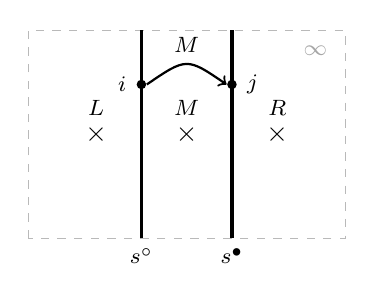
\begin{tikzpicture}[scale=1.15]
\draw[gray!55,dashed] (-1.75,-1.15) rectangle (1.75,1.15);
\draw[very thick] (-0.5,-1.15) -- (-0.5,1.15);
\draw[very thick] ( 0.5,-1.15) -- ( 0.5,1.15);
\node[below] at (-0.5,-1.15) {\footnotesize $s^{\circ}$};
\node[below] at ( 0.5,-1.15) {\footnotesize $s^{\bullet}$};
\foreach \x in {-1,0,1}{\node at (\x,0) {$\times$};}
\node[above] at (-1,0.10) {\footnotesize $L$};
\node[above] at ( 0,0.10) {\footnotesize $M$};
\node[above] at ( 1,0.10) {\footnotesize $R$};
\fill (-0.5,0.55) circle (1.5pt);  \node[left]  at (-0.56,0.55) {\footnotesize $i$};
\fill ( 0.5,0.55) circle (1.5pt);  \node[right] at ( 0.56,0.55) {\footnotesize $j$};
\draw[->,thick] (-0.44,0.55) .. controls (0,0.85) .. (0.44,0.55);
\node[above] at (0,0.80) {\footnotesize $M$};
\node[gray!70] at (1.42,0.92) {\footnotesize $\infty$};
\end{tikzpicture}
\medskip
\caption{The chart for the algebra $\mathcal B$. A distinguished corner of the pillowcase is sent to infinity,
leaving the other three corners ($\times$) in the plane. The arcs $s^{\circ},s^{\bullet}$ of the arc system cut the
chart into three faces, one for each remaining corner, labelled $L$, $M$ and $R$. In the chart used throughout
(\S\ref{ss:explicit}) the corner at infinity is $(0,\pi)$, and the faces $L$, $M$ and $R$ contain the corners
$(\pi,\pi)$, $(\pi,0)$ and $(0,0)$; Section~\ref{sec:khovanov} compares with the invariants of~\cite{KWZ} in the
normalization in which $(\pi,\pi)$ is the special puncture (\S\ref{ss:kh-smith}). A generator is an intersection
of a curve with $s^{\circ}$ or $s^{\bullet}$ and carries the idempotent $\iota_\circ$ or $\iota_\bullet$; a segment
running from $i$ to $j$ through the face $X$ contributes an arrow $i\xrightarrow{X^{k}}j$, where $k$ counts the
crossings of the arcs. Each of the faces $L$ and $R$ is bounded by a single arc of the system, so their words
join generators of equal idempotent; the face $M$ is bounded by both arcs.}
\label{fig:chart}
\end{figure}

An immersed curve in the chart that misses the corners determines an object of the category
$\operatorname{Tw}(\mathcal B)$ of twisted complexes in the standard way~\cite{KWZ}: its intersections with the arc
system are the generators, each carrying $\iota_\circ$ or $\iota_\bullet$ according to the arc it meets, and a
segment of the curve running from one intersection to the next through the face $X$ contributes the arrow
labelled by the corresponding power of $X$. Each pillowcase intersection has two lifts to the torus double cover,
interchanged by the elliptic involution $\rho$, so intersection counts on the torus are twice those on the
pillowcase.

A finite twisted complex is a finite idempotent module $V$ with a matrix $\delta$ over $\mathcal B$ satisfying
$\delta^2=0$; it is a type~D structure over $\mathcal B$ in the sense of~\cite{KWZ}, and we use the two descriptions
interchangeably. An entry of $\delta$ labelled by an idempotent is a unit, and Gaussian elimination along it
deletes its source and its target without changing the homotopy type; we call this a \emph{unit cancellation}. A
twisted complex is \emph{reduced} if every entry of $\delta$ is a sum of positive words. Two reduced twisted
complexes are \emph{strictly isomorphic} if an idempotent-preserving bijection of their generators carries one
differential to the other entry by entry. A reduced twisted complex is of \emph{loop type} if every generator
meets at most two arrows; each component of such a complex is then described by its \emph{word}, the sequence of
idempotents, labels and directions of its arrows read along the component, and a strict isomorphism of
loop-type complexes is decided by comparing the words of their components up to rotation and reversal.

For finite twisted complexes $X=(V_X,\delta_X)$ and $Y=(V_Y,\delta_Y)$, the morphism space
$\operatorname{Mor}(X,Y)$ consists of the matrices $f$ over $\mathcal B$ from $V_X$ to $V_Y$, with differential
$f\mapsto\delta_Yf+f\delta_X$. We write $\HF(X,Y):=H\operatorname{Mor}(X,Y)$, and we call
$\dim_{\F_2}\HF(X,Y)$, when it is finite, the \emph{pairing dimension} of $X$ with $Y$. For curves in the
position required by~\cite[Thm.~5.22]{KWZ}, Kotelskiy, Watson and Zibrowius show that
$\operatorname{Mor}(X,Y)$ is quasi-isomorphic to the Lagrangian Floer complex of the two curves, so the
pairing dimension is a Floer homology dimension. The hypotheses under which this identification is used are stated in Section~\ref{sec:khovanov}.

The endomorphism differential of $(V,\delta)$ is $D_\delta(b)=\delta b+b\delta$. A matrix $b$ over $\mathcal B$ is
a \emph{Maurer--Cartan element} for $(V,\delta)$ if
\begin{equation}\label{eq:typeD-MC}
(\delta+b)^2=D_\delta(b)+b^2=0,
\end{equation}
and then $(V,\delta+b)$ is again a twisted complex. There is no infinite series in~\eqref{eq:typeD-MC}: for a
suitable choice of Hamiltonian perturbations of the generating arcs, $\mu^1$ and all $\mu^k$ with $k\ge3$ vanish and
$\mu^2$ is concatenation of paths~\cite[\S11.5]{CHKK}. Cazassus, Herald, Kirk and Kotelskiy deduce this from
Bocklandt's description of the wrapped Fukaya category of a punctured surface~\cite[Thm.~7.6]{Bocklandt} and the
constructions of~\cite[\S3]{HKK}; the vanishing of the higher operations for a formal arc system is
in~\cite[\S3.4]{HKK}. The Maurer--Cartan elements used in Section~\ref{sec:smith} are supported near
self-intersection points of a curve, where they encode smoothings of the curve.

Kotelskiy, Watson and Zibrowius associate to a four-ended tangle $T$ in a ball type~D structures
$\widetilde{\mathrm{BN}}(T)$ and $\widetilde{\Kh}(T)$ over $\mathcal B$, invariants of $T$ up to homotopy
equivalence, with $\widetilde{\Kh}(T)$ the mapping cone of $H\cdot\mathrm{id}$ on
$\widetilde{\mathrm{BN}}(T)$~\cite[Def.~6.5]{KWZ}; both are represented by immersed curves, possibly with local
systems, in the four-punctured sphere~\cite{KWZ}. Their geometric pairing
theorem~\cite[Thm.~1.9]{KWZ} computes reduced Khovanov homology of a link $L=T_1\cup T_2$ obtained by gluing two
such tangles as
\[
\widetilde{\Kh}(L;\F_2)\cong\HF\bigl(\widetilde{\Kh}(mT_1),\widetilde{\mathrm{BN}}(T_2)\bigr),
\]
where $m$ denotes the mirror. For rational tangles these curves are the perturbed traceless character varieties,
$\widetilde{\mathrm{BN}}$ corresponding to the tangle and $\widetilde{\Kh}$ to the tangle with an
earring~\cite[\S1.8; for $\widetilde{\mathrm{BN}}$ also \S8.2, Prop.~8.3]{KWZ}, up to the identification of charts made in Section~\ref{sec:khovanov}.
Section~\ref{sec:khovanov} compares Smith's curve, with a Maurer--Cartan element, to
$\widetilde{\mathrm{BN}}(Q_{1/3}+Q_{1/q})$.

\subsection{The knots}\label{ss:knots}
For odd $q\ge3$ the pretzel knot $P(-2,3,q)$ is the numerator closure
\begin{equation}\label{eq:family}
P(-2,3,q)=\operatorname{num}\bigl(Q_{-1/2}+Q_{1/3}+Q_{1/q}\bigr)
\end{equation}
of a sum of rational tangles, in the convention of \S\ref{ss:smith-chart}; we write $K_q=P(-2,3,q)$. Its first two
members are the torus knots $P(-2,3,3)=T(3,4)$ and $P(-2,3,5)=T(3,5)$, and for $q\ge7$ it is
hyperbolic~\cite[Prop.~4.5]{WuebbenII}. Section~\ref{sec:smith} uses the decomposition~\eqref{eq:family} with the
earring on $Q_{-1/2}$. The companion paper~\cite{WuebbenII} uses a different decomposition, obtained from Hedden,
Herald and Kirk's decomposition of $T(3,5)$ by regluing, in which no bounding cochain is needed.

\section{Smith's decomposition}\label{sec:smith}

This section treats Smith's decomposition~\eqref{eq:family} of $K_q$, with the earring on $Q_{-1/2}$: the
piecewise-linear model of Smith's curve (\S\ref{ss:models}), its pairing dimension with zero bounding cochain at
$q=7$ (\S\ref{sec:typeD}), and the Maurer--Cartan elements selected by a second closure
(\S\ref{ss:second-closure}).  Sections~\ref{ss:correspondence} and~\ref{ss:yoneda}, on the triple point of
a Lagrangian correspondence and on a Yoneda reduction, concern the formal route to identifying the assigned
object and can be skipped on a first reading.

\subsection{Piecewise-linear models and Smith's cross-resolution}\label{ss:models}
We work in Smith's coordinates \eqref{eq:smith-coords}, with the corner rule for rational lines and
the fiber-product description of Conway sums recalled in \S\ref{ss:smith-chart}.  As Smith does, we
call the images of the lines $\gamma=0$ and $\gamma=\pi$ the \emph{edges} of the pillowcase, and the
circles of representations that a Conway sum acquires over them \emph{edge circles}
\cite[Thms.~3.15 and 3.26]{Smith}.  Smith's perturbation performs the cross-resolution
(\S\ref{ss:smith-chart}) of each internal edge circle \cite[Thm.~4.22]{Smith}; we call the two arcs crossing
once that replace the circle \emph{connectors}, and the remaining arcs of the resolved curve, which come from the fiber
product, \emph{inherited strands}.  The earring curve $E_r$ of $\Qh{r}$ is a Herald--Kirk
figure-eight, the doubled arc closing around the two end corners, with one pinch \cite[Def.~6.7]{HK}; this
specifies the immersed curve only, and its bounding cochain is discussed after
Proposition~\ref{prop:q7-typeD}.  In Smith's notation $\Qh{r}$ is the hat of $Q_r$ (the tangle
glued into the cobordism of \cite[Fig.~11a]{Smith}, with curve the reflection of the line of $Q_r$ by
$(\gamma,\theta)\mapsto(\gamma,-\theta)$ \cite[Lem.~2.31]{Smith}), the earring is his $\natural$, and $\Rnat$
denotes his perturbed character variety of a tangle carrying the earring, so that
$E_r=\Rnat(\Qh{r})$.  The closing tangle enters the pairing through its
mirror image, so $E_r$ surrounds the line of $Q_{-r}$ (\S\ref{ss:kh-smith}); for instance
$E_{-1/2}=\Rnat(\Qh{-1/2})$ lies along the line of slope $1/2$.

Write $L_{q,\mathrm{PL}}$ for the piecewise-linear curve obtained from the lines of slopes $1/3$ and
$1/q$ through $(0,0)$ by the fiber product and the crosswise joining at every edge circle.  These
lines are the translates by $(0,\pi)$ of the lines of $Q_{1/3}$ and $Q_{1/q}$, and since the fiber
product adds the $\theta$-coordinates the two shifts cancel: both fiber products have the same image
and the same edge circles.  The model represents Smith's perturbed curve for negative values of his
perturbation parameter (Remark~\ref{rem:sign}).  The earring curve $E_{-1/2}$ is one immersed
circle with one pinch; the model $L_{q,\mathrm{PL}}$ has $q-1$ resolved edge circles and is a single proper
immersed arc.  It has $40$, $82$ and $240$ transverse self-intersections at
$q=5,7,11$.  These are counts for the model: the number is not invariant under regular homotopy, and a
numerical trace of Smith's perturbed curve at $q=7$ has $50$ (Remark~\ref{rem:analytic}).  At $q=7$
the model also has twelve tangential self-contacts on the edges, where connectors meet inherited
strands without crossing; we remove them by a small perturbation that creates no crossings.  We
require $\gcd(q,3)=1$, since otherwise corner circles appear; this excludes $q=3,9,15,\dots$ from the
members computed here, but not from~\cite[Thm.~1.1]{WuebbenII}.

\begin{proposition}[Smith's cross-resolution and the model]\label{prop:smith-main}
Let $q$ be odd and $\gcd(q,3)=1$.
\begin{enumerate}
\item[(a)] The fiber product of the rational lines of slopes $1/3$ and $1/q$ has $q-1$ edge circles,
all internal, and no corner circles.
\item[(b)] For all sufficiently small nonzero values $t$ of Smith's $C_3$-perturbation parameter,
after an arbitrarily small additional perturbation where Smith's construction requires one,
$\Rp_t(Q_{1/3}+Q_{1/q})$ contains a subspace homeomorphic to the curve obtained from the fiber
product by replacing each internal circle with two intervals joined to its ends crosswise; this is
the crosswise joining used to define $L_{q,\mathrm{PL}}$, and the components of this subspace are the
\emph{main components}.  As $t\to0$ the image of each new interval approaches
the image of the corresponding circle.  The remaining components are circles, the \emph{auxiliary
components}.
\item[(c)] For a fixed complementary tangle, there is an arbitrarily small perturbation of it for
which the Lagrangian Floer homology of its curve with $\Rp_t(Q_{1/3}+Q_{1/q})$ equals that with the main
components.
This remains valid when either tangle carries an earring.
\end{enumerate}
\end{proposition}

\begin{proof}
Smith identifies the two rational character varieties with straight intervals of slopes $1/3$ and
$1/q$ \cite[Prop.~2.27]{Smith}, and rational tangles of finite slope form a good pair, that is, satisfy
Smith's transversality conditions for a sum \cite[Def.~3.16]{Smith}, without
preliminary perturbations \cite[example following Thm.~3.26]{Smith}.  Because the denominators $3$ and
$q$ are coprime, the sum has no corner circles \cite[discussion following Prop.~5.8]{Smith}, so every
edge circle is internal.  This is (a).  For $t>0$, part (b) is Smith's cross-resolution theorem
\cite[Thm.~4.22]{Smith}, together with his remark preceding \cite[Thm.~4.20]{Smith} that an
arbitrarily small additional perturbation makes the relevant spaces manifolds when transversality
fails.  For $t<0$ it follows from the case of $-t$ by the homeomorphism $\hat\sm$ of
Remark~\ref{rem:sign}, which maps $\Rp_{-t}(Q_{1/3}+Q_{1/q})$ onto $\Rp_t(Q_{1/3}+Q_{1/q})$ and the
unperturbed fiber product onto itself.  Part (c) is Smith's auxiliary-component result
\cite[Prop.~5.7]{Smith}, which includes the earring case; its proof uses only that the auxiliary
components converge to finitely many points of $\Pst$ as $t\to0$, and by the same homeomorphism this
also holds for $t<0$.
\end{proof}

Smith states informally that \cite[Thm.~4.22]{Smith} determines the image of the perturbed curve up
to regular homotopy (\cite[caption of Fig.~3]{Smith} and the outline of the proof in his
introduction); the formal statement gives the homeomorphism type and the convergence in (b).  We use
$L_{q,\mathrm{PL}}$ as a representative of the regular-homotopy class of the main components, but no proof
below depends on
this identification; at $q=7$ the type-D encoding of a traced copy of Smith's curve is strictly
isomorphic to that of $L_{7,\mathrm{PL}}$ (Remark~\ref{rem:analytic}).

\begin{remark}[The sign of the perturbation]\label{rem:sign}
For the configuration $C_3$ of \S\ref{ss:smith-chart}, write
$C_{3,t}$ for its perturbed character variety.  Its representations are
parametrized by the images of the meridians $a,b,c$ of the outer sphere and of a meridian $x$ of the
first inner sphere: the perturbation element is $p=\exp\bigl(t\operatorname{Im}(ac^{-1}x)\bigr)$, the
remaining meridians are $d=ca^{-1}b$ and $y=xp^{-1}a^{-1}pb$, and the perturbed variety is cut out by
$\operatorname{Re}(y)=0$ \cite[Prop.~4.1 and (4.1.1)]{Smith}.  The substitution
$\sm\colon(x,t)\mapsto(-x,-t)$ leaves $p$ and $d$ unchanged and replaces $y$ by $-y$, so it maps the
perturbed variety for $t$ onto that for $-t$.  It is the identity on $P_3$, and a direct computation
with Smith's boundary words \cite[Fig.~20]{Smith} shows that it acts on $P_1$ and on $P_2$ by the
translation $(\gamma,\theta)\mapsto(\gamma,\theta+\pi)$.  For odd $q$ a line of slope $1/q$ is
invariant under translation by $(\pi,\pi)$, so translation by $(0,\pi)$ carries the line of slope
$1/q$ through $(0,0)$ to the line through $(\pi,0)$ and $(0,\pi)$.  Consequently $\sm$ carries the
composition of $C_{3,t}$ with the lines of slopes $1/3$ and $1/q$ through $(0,0)$, for $t>0$, onto the
composition of $C_{3,-t}$ with the lines of $Q_{1/3}$ and $Q_{1/q}$, without moving the image in $P_3$.
Hence the piecewise-linear model, which is built from the lines through $(0,0)$ and compared with
their composition for $t>0$, represents the main component of $\Rp_t(Q_{1/3}+Q_{1/q})$ in Smith's
coordinates for small $t<0$, which is the convention of \S\ref{ss:smith-chart}.

The substitution $b\mapsto-b$ is also a symmetry of Smith's equations for each $t$, since $p$ does not
involve $b$ and $y$ changes sign; it translates each of $P_1,P_2,P_3$ by
$(\gamma,\theta)\mapsto(\gamma+\pi,\theta)$.  The composite $\hat\sm\colon(b,x,t)\mapsto(-b,-x,-t)$
therefore translates $P_1$ and $P_2$ by $(\pi,\pi)$, which preserves the lines of $Q_{1/3}$ and
$Q_{1/q}$, and $P_3$ by $(\pi,0)$, so the curve for $t>0$ is the translate by $(\pi,0)$ of the curve
for $-t$.  This translation is a symplectomorphism of $\Pst$ that permutes the corners; its effect on
pairing dimensions is recorded in Remark~\ref{rem:sign-pairings}.
\end{remark}

\begin{figure}[ht]
\centering
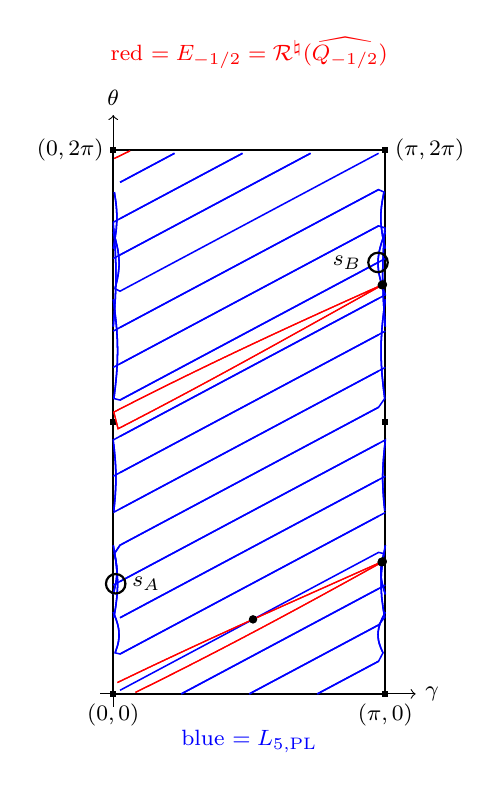
\begin{tikzpicture}[scale=1.1]
% drawn from the piecewise-linear model at q = 5
\draw[thick] (0,0) rectangle (3.14159,6.28319);
\foreach \y in {0,3.14159,6.28319}{\fill (-0.035,\y-0.035) rectangle (0.035,\y+0.035); \fill (3.14159-0.035,\y-0.035) rectangle (3.14159+0.035,\y+0.035);}
\node[below] at (0,0) {\footnotesize $(0,0)$};
\node[below] at (3.1416,0) {\footnotesize $(\pi,0)$};
\node[left] at (0,6.2832) {\footnotesize $(0,2\pi)$};
\node[right] at (3.1416,6.2832) {\footnotesize $(\pi,2\pi)$};
\draw[->] (-0.15,0)--(3.4916,0) node[right] {\footnotesize $\gamma$};
\draw[->] (0,-0.15)--(0,6.6832) node[above] {\footnotesize $\theta$};
\draw[blue,line width=0.55pt] (0.0000,5.4454) -- (0.1571,5.5292) -- (0.3142,5.6130) -- (0.4712,5.6968) -- (0.6283,5.7805) -- (0.7854,5.8643) -- (0.9425,5.9481) -- (1.0996,6.0319) -- (1.2566,6.1156) -- (1.4137,6.1994) -- (1.4923,6.2413);
\draw[blue,line width=0.55pt] (1.5708,0.0000) -- (1.7279,0.0838) -- (1.8850,0.1676) -- (2.0420,0.2513) -- (2.1991,0.3351) -- (2.3562,0.4189) -- (2.5133,0.5027) -- (2.6704,0.5864) -- (2.8274,0.6702) -- (2.9845,0.7540) -- (3.0631,0.7959);
\draw[blue,line width=0.55pt] (3.1336,0.8836) -- (3.1150,0.9948) -- (3.1000,1.1126) -- (3.0923,1.2305) -- (3.0926,1.3352) -- (3.0974,1.4137) -- (3.1056,1.4923) -- (3.1186,1.5839) -- (3.1411,1.7148);
\draw[blue,line width=0.55pt] (3.1402,4.5553) -- (3.1221,4.4113) -- (3.1092,4.2935) -- (3.1012,4.2019) -- (3.0937,4.0710) -- (3.0916,3.9532) -- (3.0947,3.8223) -- (3.1030,3.6914) -- (3.1173,3.5474) -- (3.1341,3.4099) -- (3.0631,3.3091) -- (2.9060,3.2254) -- (2.7489,3.1416) -- (2.5918,3.0578) -- (2.4347,2.9740) -- (2.2777,2.8903) -- (2.1206,2.8065) -- (1.9635,2.7227) -- (1.8064,2.6389) -- (1.6493,2.5552) -- (1.4923,2.4714) -- (1.3352,2.3876) -- (1.1781,2.3038) -- (1.0210,2.2201) -- (0.8639,2.1363) -- (0.7069,2.0525) -- (0.5498,1.9687) -- (0.3927,1.8850) -- (0.2356,1.8012) -- (0.0785,1.7174) -- (0.0135,1.6205) -- (0.0299,1.5420) -- (0.0392,1.4713) -- (0.0418,1.4085) -- (0.0394,1.3535) -- (0.0339,1.3064) -- (0.0258,1.2593) -- (0.0004,1.1493);
\draw[blue,line width=0.55pt] (0.0011,5.1417) -- (0.0163,5.2281) -- (0.0338,5.3538) -- (0.0411,5.4559) -- (0.0412,5.5423) -- (0.0363,5.6208) -- (0.0273,5.6994) -- (0.0126,5.7936);
\draw[blue,line width=0.55pt] (0.0785,5.9062) -- (0.2356,5.9900) -- (0.3927,6.0737) -- (0.5498,6.1575) -- (0.7069,6.2413);
\draw[blue,line width=0.55pt] (0.7854,0.0000) -- (0.9425,0.0838) -- (1.0996,0.1676) -- (1.2566,0.2513) -- (1.4137,0.3351) -- (1.5708,0.4189) -- (1.7279,0.5027) -- (1.8850,0.5864) -- (2.0420,0.6702) -- (2.1991,0.7540) -- (2.3562,0.8378) -- (2.5133,0.9215) -- (2.6704,1.0053) -- (2.8274,1.0891) -- (2.9845,1.1729) -- (3.0631,1.2147);
\draw[blue,line width=0.55pt] (3.1416,5.0265) -- (2.9845,4.9428) -- (2.8274,4.8590) -- (2.6704,4.7752) -- (2.5133,4.6914) -- (2.3562,4.6077) -- (2.1991,4.5239) -- (2.0420,4.4401) -- (1.8850,4.3563) -- (1.7279,4.2726) -- (1.5708,4.1888) -- (1.4137,4.1050) -- (1.2566,4.0212) -- (1.0996,3.9375) -- (0.9425,3.8537) -- (0.7854,3.7699) -- (0.6283,3.6861) -- (0.4712,3.6024) -- (0.3142,3.5186) -- (0.1571,3.4348) -- (0.0785,3.3929);
\draw[blue,line width=0.55pt] (0.0075,3.4099) -- (0.0243,3.5474) -- (0.0385,3.6914) -- (0.0469,3.8223) -- (0.0500,3.9532) -- (0.0479,4.0710) -- (0.0404,4.2019) -- (0.0324,4.2935) -- (0.0194,4.4113) -- (0.0014,4.5553);
\draw[blue,line width=0.55pt] (0.0005,1.7148) -- (0.0229,1.5839) -- (0.0360,1.4923) -- (0.0442,1.4137) -- (0.0489,1.3352) -- (0.0493,1.2305) -- (0.0416,1.1126) -- (0.0266,0.9948) -- (0.0080,0.8836);
\draw[blue,line width=0.55pt] (0.0785,0.8796) -- (0.2356,0.9634) -- (0.3927,1.0472) -- (0.5498,1.1310) -- (0.7069,1.2147) -- (0.8639,1.2985) -- (1.0210,1.3823) -- (1.1781,1.4661) -- (1.3352,1.5499) -- (1.4923,1.6336) -- (1.6493,1.7174) -- (1.8064,1.8012) -- (1.9635,1.8850) -- (2.1206,1.9687) -- (2.2777,2.0525) -- (2.4347,2.1363) -- (2.5918,2.2201) -- (2.7489,2.3038) -- (2.9060,2.3876) -- (3.0631,2.4714);
\draw[blue,line width=0.55pt] (3.1416,3.7699) -- (2.9845,3.6861) -- (2.8274,3.6024) -- (2.6704,3.5186) -- (2.5133,3.4348) -- (2.3562,3.3510) -- (2.1991,3.2673) -- (2.0420,3.1835) -- (1.8850,3.0997) -- (1.7279,3.0159) -- (1.5708,2.9322) -- (1.4137,2.8484) -- (1.2566,2.7646) -- (1.0996,2.6808) -- (0.9425,2.5970) -- (0.7854,2.5133) -- (0.6283,2.4295) -- (0.4712,2.3457) -- (0.3142,2.2619) -- (0.1571,2.1782) -- (0.0785,2.1363);
\draw[blue,line width=0.55pt] (0.0000,4.1888) -- (0.1571,4.2726) -- (0.3142,4.3563) -- (0.4712,4.4401) -- (0.6283,4.5239) -- (0.7854,4.6077) -- (0.9425,4.6914) -- (1.0996,4.7752) -- (1.2566,4.8590) -- (1.4137,4.9428) -- (1.5708,5.0265) -- (1.7279,5.1103) -- (1.8850,5.1941) -- (2.0420,5.2779) -- (2.1991,5.3617) -- (2.3562,5.4454) -- (2.5133,5.5292) -- (2.6704,5.6130) -- (2.8274,5.6968) -- (2.9845,5.7805) -- (3.0631,5.8224);
\draw[blue,line width=0.55pt] (3.1258,5.7936) -- (3.1072,5.6994) -- (3.0959,5.6208) -- (3.0898,5.5423) -- (3.0898,5.4559) -- (3.0936,5.4009) -- (3.1075,5.2988) -- (3.1211,5.2281) -- (3.1402,5.1417);
\draw[blue,line width=0.55pt] (3.1411,1.1493) -- (3.1174,1.2278) -- (3.1036,1.2828) -- (3.0950,1.3299) -- (3.0900,1.3771) -- (3.0896,1.4399) -- (3.0941,1.4870) -- (3.1040,1.5420) -- (3.1247,1.6205) -- (3.0631,1.6336) -- (2.9060,1.5499) -- (2.7489,1.4661) -- (2.5918,1.3823) -- (2.4347,1.2985) -- (2.2777,1.2147) -- (2.1206,1.1310) -- (1.9635,1.0472) -- (1.8064,0.9634) -- (1.6493,0.8796) -- (1.4923,0.7959) -- (1.3352,0.7121) -- (1.1781,0.6283) -- (1.0210,0.5445) -- (0.8639,0.4608) -- (0.7069,0.3770) -- (0.5498,0.2932) -- (0.3927,0.2094) -- (0.2356,0.1257) -- (0.0785,0.0419) -- (0.0785,0.0419) -- (0.2356,0.1257) -- (0.3927,0.2094) -- (0.5498,0.2932) -- (0.7069,0.3770) -- (0.8639,0.4608) -- (1.0210,0.5445) -- (1.1781,0.6283) -- (1.3352,0.7121) -- (1.4923,0.7959) -- (1.6493,0.8796) -- (1.8064,0.9634) -- (1.9635,1.0472) -- (2.1206,1.1310) -- (2.2777,1.2147) -- (2.4347,1.2985) -- (2.5918,1.3823) -- (2.7489,1.4661) -- (2.9060,1.5499) -- (3.0631,1.6336);
\draw[blue,line width=0.55pt] (3.1247,1.6205) -- (3.1040,1.5420) -- (3.0941,1.4870) -- (3.0896,1.4399) -- (3.0900,1.3771) -- (3.0950,1.3299) -- (3.1036,1.2828) -- (3.1174,1.2278) -- (3.1411,1.1493);
\draw[blue,line width=0.55pt] (3.1402,5.1417) -- (3.1211,5.2281) -- (3.1075,5.2988) -- (3.0936,5.4009) -- (3.0898,5.4559) -- (3.0898,5.5423) -- (3.0959,5.6208) -- (3.1072,5.6994) -- (3.1258,5.7936) -- (3.0631,5.8224) -- (2.9060,5.7386) -- (2.7489,5.6549) -- (2.5918,5.5711) -- (2.4347,5.4873) -- (2.2777,5.4035) -- (2.1206,5.3198) -- (1.9635,5.2360) -- (1.8064,5.1522) -- (1.6493,5.0684) -- (1.4923,4.9847) -- (1.3352,4.9009) -- (1.1781,4.8171) -- (1.0210,4.7333) -- (0.8639,4.6496) -- (0.7069,4.5658) -- (0.5498,4.4820) -- (0.3927,4.3982) -- (0.2356,4.3145) -- (0.0785,4.2307);
\draw[blue,line width=0.55pt] (0.0000,2.0944) -- (0.1571,2.1782) -- (0.3142,2.2619) -- (0.4712,2.3457) -- (0.6283,2.4295) -- (0.7854,2.5133) -- (0.9425,2.5970) -- (1.0996,2.6808) -- (1.2566,2.7646) -- (1.4137,2.8484) -- (1.5708,2.9322) -- (1.7279,3.0159) -- (1.8850,3.0997) -- (2.0420,3.1835) -- (2.1991,3.2673) -- (2.3562,3.3510) -- (2.5133,3.4348) -- (2.6704,3.5186) -- (2.8274,3.6024) -- (2.9845,3.6861) -- (3.0631,3.7280);
\draw[blue,line width=0.55pt] (3.1416,2.5133) -- (2.9845,2.4295) -- (2.8274,2.3457) -- (2.6704,2.2619) -- (2.5133,2.1782) -- (2.3562,2.0944) -- (2.1991,2.0106) -- (2.0420,1.9268) -- (1.8850,1.8431) -- (1.7279,1.7593) -- (1.5708,1.6755) -- (1.4137,1.5917) -- (1.2566,1.5080) -- (1.0996,1.4242) -- (0.9425,1.3404) -- (0.7854,1.2566) -- (0.6283,1.1729) -- (0.4712,1.0891) -- (0.3142,1.0053) -- (0.1571,0.9215) -- (0.0785,0.8796);
\draw[blue,line width=0.55pt] (0.0080,0.8836) -- (0.0266,0.9948) -- (0.0416,1.1126) -- (0.0493,1.2305) -- (0.0489,1.3352) -- (0.0442,1.4137) -- (0.0360,1.4923) -- (0.0229,1.5839) -- (0.0005,1.7148);
\draw[blue,line width=0.55pt] (0.0014,4.5553) -- (0.0194,4.4113) -- (0.0324,4.2935) -- (0.0404,4.2019) -- (0.0479,4.0710) -- (0.0500,3.9532) -- (0.0469,3.8223) -- (0.0385,3.6914) -- (0.0243,3.5474) -- (0.0075,3.4099) -- (0.0785,3.3929) -- (0.2356,3.4767) -- (0.3927,3.5605) -- (0.5498,3.6442) -- (0.7069,3.7280) -- (0.8639,3.8118) -- (1.0210,3.8956) -- (1.1781,3.9794) -- (1.3352,4.0631) -- (1.4923,4.1469) -- (1.6493,4.2307) -- (1.8064,4.3145) -- (1.9635,4.3982) -- (2.1206,4.4820) -- (2.2777,4.5658) -- (2.4347,4.6496) -- (2.5918,4.7333) -- (2.7489,4.8171) -- (2.9060,4.9009) -- (3.0631,4.9847);
\draw[blue,line width=0.55pt] (3.1416,1.2566) -- (2.9845,1.1729) -- (2.8274,1.0891) -- (2.6704,1.0053) -- (2.5133,0.9215) -- (2.3562,0.8378) -- (2.1991,0.7540) -- (2.0420,0.6702) -- (1.8850,0.5864) -- (1.7279,0.5027) -- (1.5708,0.4189) -- (1.4137,0.3351) -- (1.2566,0.2513) -- (1.0996,0.1676) -- (0.9425,0.0838) -- (0.7854,0.0000);
\draw[blue,line width=0.55pt] (0.7069,6.2413) -- (0.5498,6.1575) -- (0.3927,6.0737) -- (0.2356,5.9900) -- (0.0785,5.9062);
\draw[blue,line width=0.55pt] (0.0126,5.7936) -- (0.0273,5.6994) -- (0.0363,5.6208) -- (0.0412,5.5423) -- (0.0411,5.4559) -- (0.0338,5.3538) -- (0.0163,5.2281) -- (0.0011,5.1417);
\draw[blue,line width=0.55pt] (0.0004,1.1493) -- (0.0258,1.2593) -- (0.0339,1.3064) -- (0.0394,1.3535) -- (0.0418,1.4085) -- (0.0392,1.4713) -- (0.0299,1.5420) -- (0.0135,1.6205) -- (0.0785,1.7174) -- (0.2356,1.8012) -- (0.3927,1.8850) -- (0.5498,1.9687) -- (0.7069,2.0525) -- (0.8639,2.1363) -- (1.0210,2.2201) -- (1.1781,2.3038) -- (1.3352,2.3876) -- (1.4923,2.4714) -- (1.6493,2.5552) -- (1.8064,2.6389) -- (1.9635,2.7227) -- (2.1206,2.8065) -- (2.2777,2.8903) -- (2.4347,2.9740) -- (2.5918,3.0578) -- (2.7489,3.1416) -- (2.9060,3.2254) -- (3.0631,3.3091);
\draw[blue,line width=0.55pt] (3.1341,3.4099) -- (3.1173,3.5474) -- (3.1030,3.6914) -- (3.0947,3.8223) -- (3.0916,3.9532) -- (3.0937,4.0710) -- (3.1012,4.2019) -- (3.1092,4.2935) -- (3.1221,4.4113) -- (3.1402,4.5553);
\draw[blue,line width=0.55pt] (3.1411,1.7148) -- (3.1186,1.5839) -- (3.1056,1.4923) -- (3.0974,1.4137) -- (3.0926,1.3352) -- (3.0923,1.2305) -- (3.1000,1.1126) -- (3.1150,0.9948) -- (3.1336,0.8836) -- (3.0631,0.7959) -- (2.9060,0.7121) -- (2.7489,0.6283) -- (2.5918,0.5445) -- (2.4347,0.4608) -- (2.2777,0.3770) -- (2.1206,0.2932) -- (1.9635,0.2094) -- (1.8064,0.1257) -- (1.6493,0.0419) -- (1.5708,0.0000);
\draw[blue,line width=0.55pt] (1.4923,6.2413) -- (1.3352,6.1575) -- (1.1781,6.0737) -- (1.0210,5.9900) -- (0.8639,5.9062) -- (0.7069,5.8224) -- (0.5498,5.7386) -- (0.3927,5.6549) -- (0.2356,5.5711) -- (0.0785,5.4873);
\draw[blue,line width=0.55pt] (0.0050,5.3800) -- (0.0151,5.2491) -- (0.0239,5.1051) -- (0.0291,4.9742) -- (0.0310,4.8433) -- (0.0293,4.7189) -- (0.0251,4.5946) -- (0.0201,4.5029) -- (0.0121,4.3851) -- (0.0008,4.2412);
\draw[blue,line width=0.55pt] (0.0067,2.1140) -- (0.0183,2.2318) -- (0.0274,2.3562) -- (0.0310,2.4871) -- (0.0291,2.5918) -- (0.0221,2.7096) -- (0.0100,2.8405) -- (0.0000,2.9322) -- (0.1571,3.0159) -- (0.3142,3.0997) -- (0.4712,3.1835) -- (0.6283,3.2673) -- (0.7854,3.3510) -- (0.9425,3.4348) -- (1.0996,3.5186) -- (1.2566,3.6024) -- (1.4137,3.6861) -- (1.5708,3.7699) -- (1.7279,3.8537) -- (1.8850,3.9375) -- (2.0420,4.0212) -- (2.1991,4.1050) -- (2.3562,4.1888) -- (2.5133,4.2726) -- (2.6704,4.3563) -- (2.8274,4.4401) -- (2.9845,4.5239) -- (3.0631,4.5658);
\draw[blue,line width=0.55pt] (3.1161,4.6784) -- (3.0861,4.7726) -- (3.0679,4.8511) -- (3.0580,4.9297) -- (3.0569,4.9925) -- (3.0602,5.0396) -- (3.0682,5.0946) -- (3.0783,5.1417) -- (3.0958,5.2046) -- (3.1239,5.2870) -- (3.1393,5.3302);
\draw[blue,line width=0.55pt] (3.1408,0.9451) -- (3.1026,0.8666) -- (3.0804,0.8116) -- (3.0664,0.7645) -- (3.0584,0.7173) -- (3.0566,0.6859) -- (3.0578,0.6545) -- (3.0619,0.6231) -- (3.0709,0.5838) -- (3.0868,0.5367) -- (3.1143,0.4739) -- (3.0631,0.3770) -- (2.9060,0.2932) -- (2.7489,0.2094) -- (2.5918,0.1257) -- (2.4347,0.0419) -- (2.3562,0.0000);
\draw[blue,line width=0.55pt] (2.2777,6.2413) -- (2.1206,6.1575) -- (1.9635,6.0737) -- (1.8064,5.9900) -- (1.6493,5.9062) -- (1.4923,5.8224) -- (1.3352,5.7386) -- (1.1781,5.6549) -- (1.0210,5.5711) -- (0.8639,5.4873) -- (0.7069,5.4035) -- (0.5498,5.3198) -- (0.3927,5.2360) -- (0.2356,5.1522) -- (0.0785,5.0684);
\draw[blue,line width=0.55pt] (0.0000,1.2566) -- (0.1571,1.3404) -- (0.3142,1.4242) -- (0.4712,1.5080) -- (0.6283,1.5917) -- (0.7854,1.6755) -- (0.9425,1.7593) -- (1.0996,1.8431) -- (1.2566,1.9268) -- (1.4137,2.0106) -- (1.5708,2.0944) -- (1.7279,2.1782) -- (1.8850,2.2619) -- (2.0420,2.3457) -- (2.1991,2.4295) -- (2.3562,2.5133) -- (2.5133,2.5970) -- (2.6704,2.6808) -- (2.8274,2.7646) -- (2.9845,2.8484) -- (3.0631,2.8903);
\draw[blue,line width=0.55pt] (3.1366,2.8863) -- (3.1251,2.7751) -- (3.1158,2.6573) -- (3.1110,2.5395) -- (3.1112,2.4347) -- (3.1193,2.2777) -- (3.1274,2.1860) -- (3.1349,2.1140);
\draw[blue,line width=0.55pt] (3.1408,4.2412) -- (3.1295,4.3851) -- (3.1215,4.5029) -- (3.1165,4.5946) -- (3.1123,4.7189) -- (3.1106,4.8433) -- (3.1125,4.9742) -- (3.1177,5.1051) -- (3.1265,5.2491) -- (3.1366,5.3800) -- (3.0631,5.4035) -- (2.9060,5.3198) -- (2.7489,5.2360) -- (2.5918,5.1522) -- (2.4347,5.0684) -- (2.2777,4.9847) -- (2.1206,4.9009) -- (1.9635,4.8171) -- (1.8064,4.7333) -- (1.6493,4.6496) -- (1.4923,4.5658) -- (1.3352,4.4820) -- (1.1781,4.3982) -- (1.0210,4.3145) -- (0.8639,4.2307) -- (0.7069,4.1469) -- (0.5498,4.0631) -- (0.3927,3.9794) -- (0.2356,3.8956) -- (0.0785,3.8118);
\draw[blue,line width=0.55pt] (0.0000,2.5133) -- (0.1571,2.5970) -- (0.3142,2.6808) -- (0.4712,2.7646) -- (0.6283,2.8484) -- (0.7854,2.9322) -- (0.9425,3.0159) -- (1.0996,3.0997) -- (1.2566,3.1835) -- (1.4137,3.2673) -- (1.5708,3.3510) -- (1.7279,3.4348) -- (1.8850,3.5186) -- (2.0420,3.6024) -- (2.1991,3.6861) -- (2.3562,3.7699) -- (2.5133,3.8537) -- (2.6704,3.9375) -- (2.8274,4.0212) -- (2.9845,4.1050) -- (3.0631,4.1469);
\draw[blue,line width=0.55pt] (3.1416,2.0944) -- (2.9845,2.0106) -- (2.8274,1.9268) -- (2.6704,1.8431) -- (2.5133,1.7593) -- (2.3562,1.6755) -- (2.1991,1.5917) -- (2.0420,1.5080) -- (1.8850,1.4242) -- (1.7279,1.3404) -- (1.5708,1.2566) -- (1.4137,1.1729) -- (1.2566,1.0891) -- (1.0996,1.0053) -- (0.9425,0.9215) -- (0.7854,0.8378) -- (0.6283,0.7540) -- (0.4712,0.6702) -- (0.3142,0.5864) -- (0.1571,0.5027) -- (0.0785,0.4608);
\draw[blue,line width=0.55pt] (0.0217,0.4739) -- (0.0482,0.5524) -- (0.0608,0.6074) -- (0.0665,0.6545) -- (0.0661,0.7173) -- (0.0597,0.7645) -- (0.0486,0.8116) -- (0.0310,0.8666) -- (0.0006,0.9451);
\draw[blue,line width=0.55pt] (0.0018,5.3302) -- (0.0263,5.2438) -- (0.0437,5.1732) -- (0.0546,5.1182) -- (0.0647,5.0396) -- (0.0672,4.9925) -- (0.0664,4.9297) -- (0.0585,4.8511) -- (0.0440,4.7726) -- (0.0202,4.6784) -- (0.0785,4.6496) -- (0.2356,4.7333) -- (0.3927,4.8171) -- (0.5498,4.9009) -- (0.7069,4.9847) -- (0.8639,5.0684) -- (1.0210,5.1522) -- (1.1781,5.2360) -- (1.3352,5.3198) -- (1.4923,5.4035) -- (1.6493,5.4873) -- (1.8064,5.5711) -- (1.9635,5.6549) -- (2.1206,5.7386) -- (2.2777,5.8224) -- (2.4347,5.9062) -- (2.5918,5.9900) -- (2.7489,6.0737) -- (2.9060,6.1575) -- (3.0631,6.2413) -- (3.0631,6.2413) -- (2.9060,6.1575) -- (2.7489,6.0737) -- (2.5918,5.9900) -- (2.4347,5.9062) -- (2.2777,5.8224) -- (2.1206,5.7386) -- (1.9635,5.6549) -- (1.8064,5.5711) -- (1.6493,5.4873) -- (1.4923,5.4035) -- (1.3352,5.3198) -- (1.1781,5.2360) -- (1.0210,5.1522) -- (0.8639,5.0684) -- (0.7069,4.9847) -- (0.5498,4.9009) -- (0.3927,4.8171) -- (0.2356,4.7333) -- (0.0785,4.6496);
\draw[blue,line width=0.55pt] (0.0202,4.6784) -- (0.0440,4.7726) -- (0.0585,4.8511) -- (0.0664,4.9297) -- (0.0672,4.9925) -- (0.0647,5.0396) -- (0.0546,5.1182) -- (0.0437,5.1732) -- (0.0263,5.2438) -- (0.0018,5.3302);
\draw[blue,line width=0.55pt] (0.0006,0.9451) -- (0.0310,0.8666) -- (0.0486,0.8116) -- (0.0597,0.7645) -- (0.0661,0.7173) -- (0.0665,0.6545) -- (0.0608,0.6074) -- (0.0482,0.5524) -- (0.0217,0.4739) -- (0.0785,0.4608) -- (0.2356,0.5445) -- (0.3927,0.6283) -- (0.5498,0.7121) -- (0.7069,0.7959) -- (0.8639,0.8796) -- (1.0210,0.9634) -- (1.1781,1.0472) -- (1.3352,1.1310) -- (1.4923,1.2147) -- (1.6493,1.2985) -- (1.8064,1.3823) -- (1.9635,1.4661) -- (2.1206,1.5499) -- (2.2777,1.6336) -- (2.4347,1.7174) -- (2.5918,1.8012) -- (2.7489,1.8850) -- (2.9060,1.9687) -- (3.0631,2.0525);
\draw[blue,line width=0.55pt] (3.1416,4.1888) -- (2.9845,4.1050) -- (2.8274,4.0212) -- (2.6704,3.9375) -- (2.5133,3.8537) -- (2.3562,3.7699) -- (2.1991,3.6861) -- (2.0420,3.6024) -- (1.8850,3.5186) -- (1.7279,3.4348) -- (1.5708,3.3510) -- (1.4137,3.2673) -- (1.2566,3.1835) -- (1.0996,3.0997) -- (0.9425,3.0159) -- (0.7854,2.9322) -- (0.6283,2.8484) -- (0.4712,2.7646) -- (0.3142,2.6808) -- (0.1571,2.5970) -- (0.0785,2.5552);
\draw[blue,line width=0.55pt] (0.0000,3.7699) -- (0.1571,3.8537) -- (0.3142,3.9375) -- (0.4712,4.0212) -- (0.6283,4.1050) -- (0.7854,4.1888) -- (0.9425,4.2726) -- (1.0996,4.3563) -- (1.2566,4.4401) -- (1.4137,4.5239) -- (1.5708,4.6077) -- (1.7279,4.6914) -- (1.8850,4.7752) -- (2.0420,4.8590) -- (2.1991,4.9428) -- (2.3562,5.0265) -- (2.5133,5.1103) -- (2.6704,5.1941) -- (2.8274,5.2779) -- (2.9845,5.3617) -- (3.0631,5.4035);
\draw[blue,line width=0.55pt] (3.1366,5.3800) -- (3.1265,5.2491) -- (3.1177,5.1051) -- (3.1125,4.9742) -- (3.1106,4.8433) -- (3.1123,4.7189) -- (3.1165,4.5946) -- (3.1215,4.5029) -- (3.1295,4.3851) -- (3.1408,4.2412);
\draw[blue,line width=0.55pt] (3.1349,2.1140) -- (3.1233,2.2318) -- (3.1142,2.3562) -- (3.1106,2.4871) -- (3.1125,2.5918) -- (3.1195,2.7096) -- (3.1316,2.8405) -- (3.1416,2.9322) -- (2.9845,2.8484) -- (2.8274,2.7646) -- (2.6704,2.6808) -- (2.5133,2.5970) -- (2.3562,2.5133) -- (2.1991,2.4295) -- (2.0420,2.3457) -- (1.8850,2.2619) -- (1.7279,2.1782) -- (1.5708,2.0944) -- (1.4137,2.0106) -- (1.2566,1.9268) -- (1.0996,1.8431) -- (0.9425,1.7593) -- (0.7854,1.6755) -- (0.6283,1.5917) -- (0.4712,1.5080) -- (0.3142,1.4242) -- (0.1571,1.3404) -- (0.0785,1.2985);
\draw[blue,line width=0.55pt] (0.0000,5.0265) -- (0.1571,5.1103) -- (0.3142,5.1941) -- (0.4712,5.2779) -- (0.6283,5.3617) -- (0.7854,5.4454) -- (0.9425,5.5292) -- (1.0996,5.6130) -- (1.2566,5.6968) -- (1.4137,5.7805) -- (1.5708,5.8643) -- (1.7279,5.9481) -- (1.8850,6.0319) -- (2.0420,6.1156) -- (2.1991,6.1994) -- (2.2777,6.2413);
\draw[blue,line width=0.55pt] (2.3562,0.0000) -- (2.5133,0.0838) -- (2.6704,0.1676) -- (2.8274,0.2513) -- (2.9845,0.3351) -- (3.0631,0.3770);
\draw[blue,line width=0.55pt] (3.1143,0.4739) -- (3.0868,0.5367) -- (3.0709,0.5838) -- (3.0619,0.6231) -- (3.0578,0.6545) -- (3.0566,0.6859) -- (3.0584,0.7173) -- (3.0664,0.7645) -- (3.0804,0.8116) -- (3.1026,0.8666) -- (3.1408,0.9451);
\draw[blue,line width=0.55pt] (3.1393,5.3302) -- (3.1085,5.2438) -- (3.0866,5.1732) -- (3.0729,5.1182) -- (3.0642,5.0711) -- (3.0581,5.0161) -- (3.0566,4.9690) -- (3.0618,4.8904) -- (3.0761,4.8119) -- (3.1003,4.7255) -- (3.1416,4.6077) -- (2.9845,4.5239) -- (2.8274,4.4401) -- (2.6704,4.3563) -- (2.5133,4.2726) -- (2.3562,4.1888) -- (2.1991,4.1050) -- (2.0420,4.0212) -- (1.8850,3.9375) -- (1.7279,3.8537) -- (1.5708,3.7699) -- (1.4137,3.6861) -- (1.2566,3.6024) -- (1.0996,3.5186) -- (0.9425,3.4348) -- (0.7854,3.3510) -- (0.6283,3.2673) -- (0.4712,3.1835) -- (0.3142,3.0997) -- (0.1571,3.0159) -- (0.0785,2.9740);
\draw[blue,line width=0.55pt] (0.0050,2.8863) -- (0.0165,2.7751) -- (0.0258,2.6573) -- (0.0306,2.5395) -- (0.0303,2.4347) -- (0.0223,2.2777) -- (0.0142,2.1860) -- (0.0067,2.1140);
\draw[blue,line width=0.55pt] (0.0008,4.2412) -- (0.0121,4.3851) -- (0.0201,4.5029) -- (0.0251,4.5946) -- (0.0293,4.7189) -- (0.0310,4.8433) -- (0.0291,4.9742) -- (0.0239,5.1051) -- (0.0151,5.2491) -- (0.0050,5.3800) -- (0.0000,5.4454);
\draw[red,line width=0.45pt] (0.3012,0.2526) -- (0.3699,0.2853) -- (0.4385,0.3180) -- (0.5073,0.3505) -- (0.5761,0.3829) -- (0.6450,0.4152) -- (0.7139,0.4474) -- (0.7828,0.4796) -- (0.8517,0.5119) -- (0.9261,0.5462) -- (1.0004,0.5806) -- (1.0748,0.6149) -- (1.1492,0.6493) -- (1.2264,0.6845) -- (1.3036,0.7197) -- (1.3808,0.7550) -- (1.4580,0.7902) -- (1.5273,0.8216) -- (1.5967,0.8529) -- (1.6660,0.8843) -- (1.7353,0.9157) -- (1.8101,0.9492) -- (1.8849,0.9828) -- (1.9597,1.0164) -- (2.0344,1.0499) -- (2.1093,1.0834) -- (2.1841,1.1168) -- (2.2589,1.1502) -- (2.3338,1.1837) -- (2.4076,1.2165) -- (2.4814,1.2494) -- (2.5552,1.2823) -- (2.6290,1.3152) -- (2.7028,1.3481) -- (2.7766,1.3810) -- (2.8504,1.4139) -- (2.9242,1.4468) -- (2.9980,1.4797) -- (3.0718,1.5125) -- (3.1395,1.5429);
\draw[red,line width=0.45pt] (3.0760,4.7100) -- (3.0084,4.6797) -- (2.9407,4.6494) -- (2.8730,4.6191) -- (2.8053,4.5887) -- (2.7342,4.5567) -- (2.6630,4.5246) -- (2.5919,4.4925) -- (2.5279,4.4635) -- (2.4640,4.4345) -- (2.4000,4.4055) -- (2.3361,4.3763) -- (2.2722,4.3471) -- (2.2083,4.3180) -- (2.1480,4.2903) -- (2.0878,4.2626) -- (2.0275,4.2349) -- (1.9567,4.2021) -- (1.8859,4.1693) -- (1.8151,4.1364) -- (1.7480,4.1050) -- (1.6809,4.0736) -- (1.6137,4.0422) -- (1.5467,4.0106) -- (1.4797,3.9790) -- (1.4127,3.9473) -- (1.3493,3.9171) -- (1.2860,3.8869) -- (1.2226,3.8566) -- (1.1559,3.8245) -- (1.0891,3.7923) -- (1.0224,3.7601) -- (0.9593,3.7294) -- (0.8961,3.6987) -- (0.8330,3.6679) -- (0.7701,3.6369) -- (0.7071,3.6059) -- (0.6441,3.5750) -- (0.5813,3.5437) -- (0.5184,3.5124) -- (0.4556,3.4812) -- (0.3929,3.4497) -- (0.3301,3.4181) -- (0.2674,3.3866) -- (0.2014,3.3531) -- (0.1353,3.3195) -- (0.0693,3.2859) -- (0.0068,3.2539) -- (0.0556,3.0614) -- (0.1181,3.0934) -- (0.1838,3.1275) -- (0.2496,3.1616) -- (0.3154,3.1958) -- (0.3810,3.2301) -- (0.4467,3.2645) -- (0.5123,3.2989) -- (0.5813,3.3354) -- (0.6502,3.3719) -- (0.7192,3.4084) -- (0.7880,3.4451) -- (0.8568,3.4818) -- (0.9257,3.5186) -- (0.9943,3.5556) -- (1.0630,3.5926) -- (1.1317,3.6296) -- (1.1900,3.6612) -- (1.2483,3.6928) -- (1.3066,3.7245) -- (1.3683,3.7581) -- (1.4299,3.7918) -- (1.4916,3.8254) -- (1.5532,3.8592) -- (1.6147,3.8930) -- (1.6763,3.9268) -- (1.7447,3.9645) -- (1.8130,4.0022) -- (1.8813,4.0399) -- (1.9551,4.0808) -- (2.0288,4.1217) -- (2.1025,4.1626) -- (2.1763,4.2035) -- (2.2500,4.2443) -- (2.3267,4.2871) -- (2.4035,4.3298) -- (2.4802,4.3725) -- (2.5569,4.4152) -- (2.6337,4.4579) -- (2.7104,4.5006) -- (2.7871,4.5433) -- (2.8639,4.5860) -- (2.9406,4.6288) -- (3.0173,4.6715) -- (3.0941,4.7142);
\draw[red,line width=0.45pt] (3.1124,1.5263) -- (3.0483,1.4908) -- (2.9843,1.4554) -- (2.9203,1.4199) -- (2.8563,1.3845) -- (2.7777,1.3412) -- (2.6991,1.2978) -- (2.6205,1.2545) -- (2.5563,1.2194) -- (2.4921,1.1843) -- (2.4279,1.1491) -- (2.3637,1.1140) -- (2.2849,1.0712) -- (2.2060,1.0283) -- (2.1272,0.9855) -- (2.0516,0.9448) -- (1.9760,0.9042) -- (1.9004,0.8635) -- (1.8247,0.8231) -- (1.7490,0.7827) -- (1.6733,0.7424) -- (1.6112,0.7096) -- (1.5491,0.6769) -- (1.4870,0.6441) -- (1.4249,0.6114) -- (1.3626,0.5790) -- (1.3003,0.5465) -- (1.2381,0.5141) -- (1.1758,0.4817) -- (1.1134,0.4496) -- (1.0510,0.4175) -- (0.9885,0.3854) -- (0.9261,0.3533) -- (0.8461,0.3127) -- (0.7661,0.2721) -- (0.6862,0.2316) -- (0.6260,0.2014) -- (0.5659,0.1713) -- (0.5057,0.1412) -- (0.4456,0.1111) -- (0.3826,0.0800) -- (0.3197,0.0490) -- (0.2567,0.0179);
\draw[red,line width=0.45pt] (0.1938,6.2700) -- (0.1333,6.2405) -- (0.0729,6.2111) -- (0.0124,6.1816);
\draw[red,line width=0.45pt] (0.0481,0.1310) -- (0.1114,0.1614) -- (0.1746,0.1918) -- (0.2379,0.2222) -- (0.3012,0.2526);
\draw[red,line width=0.45pt] (0.3012,0.2526) -- (0.3699,0.2853) -- (0.4385,0.3180) -- (0.5073,0.3505) -- (0.5761,0.3829) -- (0.6450,0.4152) -- (0.7139,0.4474) -- (0.7828,0.4796) -- (0.8517,0.5119) -- (0.9261,0.5462) -- (1.0004,0.5806) -- (1.0748,0.6149) -- (1.1492,0.6493) -- (1.2264,0.6845) -- (1.3036,0.7197) -- (1.3808,0.7550) -- (1.4580,0.7902) -- (1.5273,0.8216) -- (1.5967,0.8529) -- (1.6660,0.8843) -- (1.7353,0.9157) -- (1.8101,0.9492) -- (1.8849,0.9828) -- (1.9597,1.0164) -- (2.0344,1.0499) -- (2.1093,1.0834) -- (2.1841,1.1168) -- (2.2589,1.1502) -- (2.3338,1.1837) -- (2.4076,1.2165) -- (2.4814,1.2494) -- (2.5552,1.2823) -- (2.6290,1.3152) -- (2.7028,1.3481) -- (2.7766,1.3810) -- (2.8504,1.4139) -- (2.9242,1.4468) -- (2.9980,1.4797) -- (3.0718,1.5125) -- (3.1395,1.5429);
\draw[red,line width=0.45pt] (3.0760,4.7100) -- (3.0084,4.6797) -- (2.9407,4.6494) -- (2.8730,4.6191) -- (2.8053,4.5887) -- (2.7342,4.5567) -- (2.6630,4.5246) -- (2.5919,4.4925) -- (2.5279,4.4635) -- (2.4640,4.4345) -- (2.4000,4.4055) -- (2.3361,4.3763) -- (2.2722,4.3471) -- (2.2083,4.3180) -- (2.1480,4.2903) -- (2.0878,4.2626) -- (2.0275,4.2349) -- (1.9567,4.2021) -- (1.8859,4.1693) -- (1.8151,4.1364) -- (1.7480,4.1050) -- (1.6809,4.0736) -- (1.6137,4.0422) -- (1.5467,4.0106) -- (1.4797,3.9790) -- (1.4127,3.9473) -- (1.3493,3.9171) -- (1.2860,3.8869) -- (1.2226,3.8566) -- (1.1559,3.8245) -- (1.0891,3.7923) -- (1.0224,3.7601) -- (0.9593,3.7294) -- (0.8961,3.6987) -- (0.8330,3.6679) -- (0.7701,3.6369) -- (0.7071,3.6059) -- (0.6441,3.5750) -- (0.5813,3.5437) -- (0.5184,3.5124) -- (0.4556,3.4812) -- (0.3929,3.4497) -- (0.3301,3.4181) -- (0.2674,3.3866) -- (0.2014,3.3531) -- (0.1353,3.3195) -- (0.0693,3.2859) -- (0.0068,3.2539) -- (0.0556,3.0614) -- (0.1181,3.0934) -- (0.1838,3.1275) -- (0.2496,3.1616) -- (0.3154,3.1958) -- (0.3810,3.2301) -- (0.4467,3.2645) -- (0.5123,3.2989) -- (0.5813,3.3354) -- (0.6502,3.3719) -- (0.7192,3.4084) -- (0.7880,3.4451) -- (0.8568,3.4818) -- (0.9257,3.5186) -- (0.9943,3.5556) -- (1.0630,3.5926) -- (1.1317,3.6296) -- (1.1900,3.6612) -- (1.2483,3.6928) -- (1.3066,3.7245) -- (1.3683,3.7581) -- (1.4299,3.7918) -- (1.4916,3.8254) -- (1.5532,3.8592) -- (1.6147,3.8930) -- (1.6763,3.9268) -- (1.7447,3.9645) -- (1.8130,4.0022) -- (1.8813,4.0399) -- (1.9551,4.0808) -- (2.0288,4.1217) -- (2.1025,4.1626) -- (2.1763,4.2035) -- (2.2500,4.2443) -- (2.3267,4.2871) -- (2.4035,4.3298) -- (2.4802,4.3725) -- (2.5569,4.4152) -- (2.6337,4.4579) -- (2.7104,4.5006) -- (2.7871,4.5433) -- (2.8639,4.5860) -- (2.9406,4.6288) -- (3.0173,4.6715) -- (3.0941,4.7142);
\draw[red,line width=0.45pt] (3.1124,1.5263) -- (3.0483,1.4908) -- (2.9843,1.4554) -- (2.9203,1.4199) -- (2.8563,1.3845) -- (2.7777,1.3412) -- (2.6991,1.2978) -- (2.6205,1.2545) -- (2.5563,1.2194) -- (2.4921,1.1843) -- (2.4279,1.1491) -- (2.3637,1.1140) -- (2.2849,1.0712) -- (2.2060,1.0283) -- (2.1272,0.9855) -- (2.0516,0.9448) -- (1.9760,0.9042) -- (1.9004,0.8635) -- (1.8247,0.8231) -- (1.7490,0.7827) -- (1.6733,0.7424) -- (1.6112,0.7096) -- (1.5491,0.6769) -- (1.4870,0.6441) -- (1.4249,0.6114) -- (1.3626,0.5790) -- (1.3003,0.5465) -- (1.2381,0.5141) -- (1.1758,0.4817) -- (1.1134,0.4496) -- (1.0510,0.4175) -- (0.9885,0.3854) -- (0.9261,0.3533) -- (0.8461,0.3127) -- (0.7661,0.2721) -- (0.6862,0.2316) -- (0.6260,0.2014) -- (0.5659,0.1713) -- (0.5057,0.1412) -- (0.4456,0.1111) -- (0.3826,0.0800) -- (0.3197,0.0490) -- (0.2567,0.0179);
\draw[red,line width=0.45pt] (0.1938,6.2700) -- (0.1333,6.2405) -- (0.0729,6.2111) -- (0.0124,6.1816);
\draw[red,line width=0.45pt] (0.0481,0.1310) -- (0.1114,0.1614) -- (0.1746,0.1918) -- (0.2379,0.2222) -- (0.3012,0.2526);
\fill[black] (1.6137,0.8606) circle (1.4pt);
\fill[black] (3.1007,1.5255) circle (1.4pt);
\fill[black] (3.1106,1.5299) circle (1.4pt);
\fill[black] (3.1016,4.7215) circle (1.4pt);
\fill[black] (3.1121,4.7262) circle (1.4pt);
\fill[black] (3.1121,4.7242) circle (1.4pt);
\fill[black] (3.1025,4.7189) circle (1.4pt);
\fill[black] (3.1099,1.5249) circle (1.4pt);
\fill[black] (3.0995,1.5192) circle (1.4pt);
\draw[black,thick] (0.0281,1.2716) circle (3.2pt);
\draw[black,thick] (3.0568,4.9813) circle (3.2pt);
\node[right] at (0.1081,1.2716) {\footnotesize $s_A$};
\node[left] at (2.9768,4.9813) {\footnotesize $s_B$};
\node[blue] at (1.57,-0.55) {\footnotesize blue $=L_{5,\mathrm{PL}}$};
\node[red] at (1.57,7.40) {\footnotesize red $=E_{-1/2}=\Rnat(\Qh{-1/2})$};
\end{tikzpicture}
\caption{The two piecewise-linear model curves at $q=5$ on the fundamental domain
$[0,\pi]\times[0,2\pi)$ of the pillowcase, in Smith's coordinates (compare \cite[Fig.~31]{Smith}).
Blue is the model $L_{5,\mathrm{PL}}$ of Smith's perturbed curve $\Rp_t(Q_{1/3}+Q_{1/5})$, a single immersed arc with $40$
self-intersections clustered along the edges; the small arcs hugging the edges $\gamma\in\{0,\pi\}$ are
the connectors resolving the four edge circles, drawn at amplitude $\varepsilon\approx0.05$--$0.07$, and
the V-shaped turnbacks at the border are strands reflecting off the edges in the quotient.  Red is the
earring figure-eight $E_{-1/2}=\Rnat(\Qh{-1/2})$.  Across the interior the blue strands run nearly parallel to
red (slopes $8/15$ and $1/2$, crossing angle $\approx0.026$).  Solid dots are the nine intersection points of
the two curves: one interior, and two clusters of four near
$\gamma=\pi$ that merge at this scale.  The circled self-intersections $s_A,s_B$ are the support of
Computation~\ref{comp:cochains}(i).  Curves appear as several arcs because the fundamental domain folds
the double cover.}
\label{fig:pillow}
\end{figure}

\subsection{The \texorpdfstring{$Q_{1/3}$}{Q(1/3)} correspondence is not embedded}\label{ss:correspondence}
Write $P_i^*$ for the smooth locus of $P_i$, $P^-$ for a pillowcase with the sign of its symplectic
form reversed, and $C_{3,t}^{\mathrm{reg}}\iss P_1^-\times P_2^-\times P_3$ for the regular locus of
the perturbed correspondence of the three-boundary configuration $C_3$, Smith's $\mathcal R_{D_t}(C_3)^*$
\cite[Def.~4.9]{Smith}, which maps
to the product of pillowcases by a Lagrangian immersion \cite[Cor.~4.11]{Smith}.

\begin{lemma}[Reduction to a correspondence between surfaces]\label{lem:surface-reduction}
Let $A_{1/3}\iss P_1$ be the rational line of $Q_{1/3}$.  Wherever the fiber product is transverse,
\[
 F_{1/3,t}:=A_{1/3}\times_{P_1}C_{3,t}^{\mathrm{reg}}\iss P_2^-\times P_3
\]
is an immersed Lagrangian surface.  On a torus-cover chart, with $\gamma\notin\{0,\pi\}$, of Smith's
unperturbed manifold $R(C_3)^*$ \cite[Def.~3.6]{Smith} (on such a chart all representations are binary dihedral), a branch of $A_{1/3}$ has $\theta_1=\gamma/3+\nu$ for a constant $\nu$, and $F_{1/3,0}$ is the graph
of the symplectic shear $(\gamma,\eta)\mapsto(\gamma,\eta+\gamma/3+\nu)$; on compact subsets of such a
chart the projection of $F_{1/3,t}$ to $P_2$ remains a local diffeomorphism for small $|t|$.  After
composition with the rational line of $Q_{1/7}$, the complement of these graph charts lies in
neighborhoods of the six internal edge circles of Proposition~\ref{prop:smith-main} and of the two
corner endpoints of the composed arc.  If the fiber product is transverse along the entire regular
locus, the target projection $F_{1/3,t}\to P_3^*$ is proper.
\end{lemma}

\begin{proof}
Over such a chart Smith's boundary-coordinate formulas give $p_1=(\gamma,\beta)$,
$p_2=(\gamma,\theta-\beta)$ and $p_3=(\gamma,\theta)$ \cite[(3.1.1)--(3.1.6) and the proof of
Prop.~3.20]{Smith}.  Imposing $\beta=\gamma/3+\nu$ and writing
$\eta=\theta-\beta$ gives the displayed graph, which preserves $d\gamma\wedge d\theta$, so the
transverse composition is Lagrangian; the local-diffeomorphism property persists on compact subsets by
the implicit function theorem.  For $Q_{1/3}$ and $Q_{1/7}$ there are six internal edge circles, and
\cite[Thm.~4.22]{Smith} replaces precisely their neighborhoods by their cross-resolutions, as in the
construction of $L_{7,\mathrm{PL}}$.  For properness, let $\overline A_{1/3}$ be the compact rational arc and
$\overline F_{1/3,t}:=\overline A_{1/3}\times_{P_1}\mathcal R_{D_t}(C_3)$, a compact space; here
$\mathcal R_{D_t}(C_3)$ is Smith's notation for $C_{3,t}$ \cite[\S4.1]{Smith}.  The
boundary restriction of $\mathcal R_{D_t}(C_3)$ lies either in $P_1^*\times P_2^*\times P_3^*$ or in
the product of the three corner strata \cite[Prop.~4.3]{Smith} (for $t<0$ via Remark~\ref{rem:sign}), and its regular Lagrangian locus is
the former \cite[Cor.~4.11]{Smith}.  Hence $\overline F_{1/3,t}\setminus F_{1/3,t}$ maps to the corners
of $P_3$, and the inverse image of a compact subset of $P_3^*$ is compact and lies in $F_{1/3,t}$.
\end{proof}

\begin{proposition}[A triple-point obstruction]\label{prop:partial-triple}
For every sufficiently small $t<0$, the partial fiber product of Lemma~\ref{lem:surface-reduction} has
three distinct points, at each of which the fiber product is transverse, with common image
$\bigl((0,\pi/2),(0,\pi/2)\bigr)$ in $P_2^*\times P_3^*$.  Consequently $F_{1/3,t}\to P_2^-\times P_3$ is not embedded.
\end{proposition}

\begin{proof}
Put $v(\varphi)=\cos\varphi\,\mathbf i+\sin\varphi\,\mathbf k$ and fix $\gamma=0$, $\theta=\pi/2$ in
Smith's parametrization, so that $a=b=\mathbf i$ and $c=d=\mathbf j$.  For $\beta=0$ or $\pi$ write
$(\varphi,u)=(\pi/2-\alpha,\ t\sin\alpha)$ if $\beta=0$ and $(\varphi,u)=(\pi/2+\alpha,-t\sin\alpha)$ if
$\beta=\pi$.  Then $x=v(\varphi)$, the perturbation element is $p=e^{-u\mathbf j}$, and direct
quaternion multiplication shows that $y=xp^{-1}a^{-1}pb$ is purely imaginary, so
$\operatorname{Re}(y)=0$ holds identically along these two families.  On the torus cover the first
boundary value is $(\gamma_1,\theta_1)=(2u,\varphi+2u)$.

Take first $t>0$ and the line $A^0_{1/3}=\{3\theta_1-\gamma_1\in2\pi\Z\}$ through $(0,0)$, the
translate of $A_{1/3}$ by $(0,\pi)$.  Its equation $3\varphi+4u\in2\pi\Z$ gives
\begin{align*}
 3(\pi/2-\alpha)+4t\sin\alpha&=0,      &\alpha&\to\pi/2,\quad \beta=0,\\
 3(\pi/2+\alpha)-4t\sin\alpha&=2\pi,   &\alpha&\to\pi/6,\quad \beta=\pi,\\
 3(\pi/2+\alpha)-4t\sin\alpha&=4\pi,   &\alpha&\to5\pi/6,\quad \beta=\pi,
\end{align*}
with $\alpha$-derivatives $-3,3,3$ at $t=0$, so the implicit function theorem gives three solutions
for small $t>0$.  They are distinct, since their limiting $x$-values are, and none lies over a corner
of $P_1$, since $|\gamma_1|=2t\sin\alpha>0$.  Using $xp=p^{-1}x$, the second-boundary words become
$\bigl(v(\varphi+2u),v(\varphi+2u),\mathbf j,\mathbf j\bigr)$, so $p_2=(0,\pi/2)$ at all three
points, and $(a,b,c,d)=(\mathbf i,\mathbf i,\mathbf j,\mathbf j)$ gives $p_3=(0,\pi/2)$.  Since
$\partial_\beta\operatorname{Re}(y)=-2t\sin^2\alpha+O(t^2)$ and
$\partial_\alpha(3\theta_1-\gamma_1)=\pm3+O(t)$, the fiber product is transverse at all three points.
Finally, the symmetry $\sm$ of Remark~\ref{rem:sign} maps the fiber product of $A^0_{1/3}$ with
$C_{3,t}$ onto that of $A_{1/3}$ with $C_{3,-t}$, preserving distinctness, transversality and
$\gamma_1$, fixing $p_3$ and translating $p_2$ by $(0,\pi)$.  Since $(0,3\pi/2)=\rho(0,\pi/2)$, the
three image points again map to $\bigl((0,\pi/2),(0,\pi/2)\bigr)$; replacing $t$ by $-t$ gives the
statement.
\end{proof}

Gao's wrapped representability theorem \cite[Thm.~7.24 and Cor.~7.25]{Gao} applies to
\emph{admissible} correspondences, which are properly embedded, exact and cylindrical, with vanishing
relative first Chern class \cite[Def.~6.3, Def.~7.2 and the standing convention of \S7.1]{Gao}, and
whose projection to the target is proper; only the geometric composition may be immersed
\cite[Assumption~7.10]{Gao}, and the unobstructedness input \cite[Thm.~7.12]{Gao} has the same
hypotheses.  By Proposition~\ref{prop:partial-triple}, Gao's theorem cannot be invoked for
$F_{1/3,t}$, whose exactness, cylindricity and Chern class have not been checked either.  The triple
point is not generic, although the three sheets are pairwise transverse; splitting it into double
points leaves $F_{1/3,t}$ non-embedded.  Gao expects the results of his \S6 to extend to immersed
Lagrangians \cite[Rem.~6.1]{Gao}, but no immersed version of \cite[Thm.~7.24]{Gao} is stated.
Fukaya's compact theorem \cite{FukayaCorr} does not apply verbatim to $\Pst$, and the torus double
cover does not help by itself: Smith's perturbed $C_3$ variety has singular points with neighborhoods
that are cones on tori \cite[Thm.~4.16]{Smith}, and the required equivariant correspondence functor
has not been constructed \cite[\S11.5]{CHKK}.

\subsection{The pairing dimension with zero bounding cochain at \texorpdfstring{$q=7$}{q=7}}\label{sec:typeD}
We use the algebra $\mathcal B$, the arc system $s^\circ,s^\bullet$ with its faces $L,M,R$,
the twisted complexes of curves, unit cancellations, morphism complexes and pairing dimensions as in
\S\ref{ss:kwz}, ignoring gradings, and we omit exponents equal to one in arrows
$i\xrightarrow{X^k}j$.  A perturbation $b$ of a twisted complex is Maurer--Cartan exactly when
\eqref{eq:typeD-MC} holds, a finite identity.  A recorded degree is the relative quantum grading
$\gr_q$ of \cite{KWZ}, computed in the chart below, that is, with $(0,\pi)$ as the special puncture; it plays
no part in the Maurer--Cartan equation or in any pairing dimension.

\subsubsection{Finiteness of the morphism complex}
Since $\mathcal B$ is infinite dimensional, so is the morphism complex $\operatorname{Mor}(\mathcal
E,N)$ of two finite twisted complexes, and its homology need not be finite.  The \emph{identity part}
$\operatorname{Mor}^\times$ of $\operatorname{Mor}(\mathcal E,N)$ is spanned by the entries labelled
by the two vertex idempotents, and for $X\in\{L,M,R\}$ its \emph{$X$-part} $\operatorname{Mor}^X$ by
the entries labelled by positive powers of $X$.  Put $U_L=L$, $U_R=R$ and $U_M=M^2$.

\begin{lemma}[Mapping-cone reduction of the morphism complex]\label{lem:wrapped-reduction}
Let $\mathcal E$ and $N$ be reduced finite twisted complexes over $\mathcal B$.
\begin{enumerate}
\item[(a)] The differential maps $\operatorname{Mor}^\times$ into
$\operatorname{Mor}^+:=\operatorname{Mor}^L\oplus\operatorname{Mor}^M\oplus\operatorname{Mor}^R$ and
preserves each $\operatorname{Mor}^X$.  Hence $\operatorname{Mor}(\mathcal E,N)$ is the mapping cone of
a chain map $\beta\colon\operatorname{Mor}^\times\to\operatorname{Mor}^+$, where
$\operatorname{Mor}^\times$ is finite dimensional with zero differential.
\item[(b)] Each $\operatorname{Mor}^X$ is a free $\F_2[U_X]$-module of finite rank, with $U_X$ acting by
multiplication, and its differential is $\F_2[U_X]$-linear.  Consequently
$H(\operatorname{Mor}^X)\cong\F_2[U_X]^{f_X}\oplus\bigoplus_i\F_2[U_X]/(p_{X,i})$ for some $f_X\ge0$
and nonconstant polynomials $p_{X,i}$.
\item[(c)] $H\operatorname{Mor}(\mathcal E,N)$ is finite dimensional if and only if $f_L=f_M=f_R=0$,
that is, if and only if each $\operatorname{Mor}^X\otimes_{\F_2[U_X]}\F_2(U_X)$ is acyclic.  In that
case, with $e=\dim\operatorname{Mor}^\times$ and $\tau=\dim_{\F_2}H(\operatorname{Mor}^+)=\sum_{X,i}\deg
p_{X,i}$, and with $\beta_*\colon\operatorname{Mor}^\times\to H(\operatorname{Mor}^+)$ the induced map,
\begin{equation}\label{eq:wrapped-reduction}
 \dim_{\F_2}H\operatorname{Mor}(\mathcal E,N)=e+\tau-2\rk\beta_*.
\end{equation}
\end{enumerate}
\end{lemma}

\begin{proof}
Composing an idempotent entry with the positive words of $\delta_{\mathcal E}$ and $\delta_N$ gives
positive words, and a positive power of $X$ composed with a word in a different face is zero; this is
(a).  For (b), the entries of $\operatorname{Mor}^X$ joining a fixed pair of generators are the powers
$X^k$, $k\ge k_0$, of a fixed parity when $X=M$; multiplication by $U_X$ shifts $k$ by $1$ for $X=L,R$
and by $2$ for $X=M$, so $\operatorname{Mor}^X$ is free on the entries of lowest length, and the
differential commutes with $U_X$ because powers of $X$ commute.  The decomposition is the structure
theorem over the principal ideal domain $\F_2[U_X]$.  For (c), the cone gives the exact sequence
$0\to\operatorname{coker}\beta_*\to H\operatorname{Mor}(\mathcal E,N)\to\ker\beta_*\to0$, so the
homology is finite exactly when $H(\operatorname{Mor}^+)$ has no free summand, and $f_X$ is the
dimension of $H(\operatorname{Mor}^X\otimes\F_2(U_X))$ by flatness.  When $H(\operatorname{Mor}^+)$ is
finite, the sequence gives dimension $(\tau-\rk\beta_*)+(e-\rk\beta_*)$.
\end{proof}

\begin{remark}\label{rem:kwz-cone}
The mapping cone is the algebraic step preceding \cite[Thm.~5.22]{KWZ};
Lemma~\ref{lem:wrapped-reduction} records the ungraded form used here.  The torsion condition
in (c) is a genuine hypothesis: for the one-generator complex $(\iota_\circ,0)$ the endomorphism
complex $\iota_\circ\mathcal B\iota_\circ$ has $f_L=f_M=1$, and for the complex $N$ below
$\operatorname{End}(N)$ has $f_M=f_R=1$.  For every pair of complexes whose morphism homology is used
in this paper, exact computation over $\F_2[U_X]$ shows $f_L=f_M=f_R=0$ and $p_{X,i}=U_X$ for all
$i$, so that $\tau$ is the number of torsion summands.
\end{remark}

\subsubsection{The two explicit twisted complexes}\label{ss:explicit}
We send the corner $(0,\pi)$ to infinity, so that the faces $L$, $M$ and $R$ contain the corners
$(\pi,\pi)$, $(\pi,0)$ and $(0,0)$ (Figure~\ref{fig:chart}).  The curves encoded below, namely the arc $N$ with ends at
$(0,0)$ and $(\pi,0)$, its smoothings and closed earring curves, meet neither $(0,\pi)$ nor the corner
$(\pi,\pi)$ that no tangle character variety meets.  The description of~\cite[\S11.5]{CHKK} applies to any
corner, since
translations of the pillowcase permute the corners, and in either case morphisms are computed in the
wrapped category of the pillowcase with all four corners removed, so the morphism homology does not
depend on which of the two corners is at infinity.  For a slope $r$ we write $\mathcal E_r$ for the reduced
twisted complex that encodes the earring curve $E_r$ in this chart.

In this chart the model $L_{7,\mathrm{PL}}$ meets the arc system in $74$ points of the torus cover, that is, in
$37$ points of the pillowcase.  Three unit cancellations leave the $31$-generator complex $N$ whose
$\iota_\circ$ generators are $1,2,5,6,15,16,20,21,32,33$; the remaining generators in
\[
 V_N=\{0,1,\dots,10,13,14,\dots,23,26,27,30,31,\dots,36\}
\]
carry $\iota_\bullet$, and
\begin{align*}
\delta_N={}&
17\xrightarrow R18+16\xrightarrow M17+16\xrightarrow L15
+15\xrightarrow M14+14\xrightarrow R13+13\xrightarrow{M^2}10
+10\xrightarrow R9+8\xrightarrow{M^2}9\\
&+7\xrightarrow R8+6\xrightarrow M7+6\xrightarrow L5+5\xrightarrow M4+4\xrightarrow R3
+2\xrightarrow M3+2\xrightarrow L1+1\xrightarrow M0\\
&+0\xrightarrow R19+20\xrightarrow M19+20\xrightarrow L21+21\xrightarrow M22
+22\xrightarrow R23+23\xrightarrow{M^2}26+26\xrightarrow R27\\
&+30\xrightarrow{M^2}27+31\xrightarrow R30+32\xrightarrow M31
+32\xrightarrow L33+33\xrightarrow M34+34\xrightarrow R35+35\xrightarrow{M^2}36.
\end{align*}
Direct path multiplication gives $\delta_N^2=0$.  The earring curve $E_{-1/2}$ meets the arc system in eight
points, and one unit cancellation leaves a six-generator complex $\mathcal E=\mathcal E_{-1/2}$ with $\iota_\circ$
generators $5,6$, $\iota_\bullet$ generators $0,3,4,7$, and
\begin{equation}\label{eq:red-typeD}
 \delta_{\mathcal E}=3\xrightarrow{M^2}0+4\xrightarrow R3+5\xrightarrow M4
 +6\xrightarrow L5+6\xrightarrow M7+0\xrightarrow R7 ,
\end{equation}
again with $\delta_{\mathcal E}^2=0$.

\subsubsection{Smoothings and switches}\label{ss:smoothings}
A self-intersection of $L_{7,\mathrm{PL}}$ is \emph{connector--inherited} if one branch is a connector and
the other an inherited strand, and \emph{connector--connector} if both branches are connectors.  The
lift of $L_{7,\mathrm{PL}}$ to the torus double cover is a single closed immersed curve $C$ of homology class
$(21,10)$; the involution $\rho$ reverses its orientation, and each self-intersection orbit $s$ of the
model consists of two transverse double points of $C$ interchanged by $\rho$.  We label the orbits
$S_0,S_1,\dots$ in the order in which the ancillary files enumerate them (\S\ref{ss:repro}); the indices are arbitrary labels; the four orbits of Proposition~\ref{prop:q7-typeD} are identified by their coordinates, the others through the ancillary files.  Exactly one of the two
smoothings of a double point is compatible with the orientation of $C$; it splits off the loop of $C$
between the two visits.  The \emph{oriented smoothing} at $s$ performs it at both points of $s$, in
disjoint disks; the pair is $\rho$-invariant and defines a smoothing of the pillowcase curve.
Performing the other smoothing at both points gives the \emph{unoriented smoothing}.  At $38$ of the $82$
orbits the two branches lie on the same lift of the pillowcase arc, and there the oriented smoothing is
also compatible with an orientation of that arc; the four orbits below are of this kind.  A smoothing
is \emph{generator-preserving} if, after the three unit cancellations, its encoding has the same
idempotent module $V_N$; its differential then differs from $\delta_N$ by an element
$b_s\in\operatorname{End}(N)$, the \emph{switch} at $s$.  An \emph{algebraic switch} of a reduced twisted
complex $X$ is an element of $\operatorname{End}(X)$ that replaces two arrows $i\xrightarrow{Y^k}j$ and
$i'\xrightarrow{Y^k}j'$ of $\delta_X$, with $j$ and $j'$ of the same idempotent, by $i\xrightarrow{Y^k}j'$
and $i'\xrightarrow{Y^k}j$, and for which the result satisfies the Maurer--Cartan equation.  A switch is
defined by a smoothing of the curve, whereas an algebraic switch is defined by the complex alone and need not
come from a smoothing.

\begin{proposition}\label{prop:q7-typeD}
The pairing dimension of $\mathcal E$ with $N$ is
\[
 \dim_{\F_2}H\operatorname{Mor}_{\operatorname{Tw}(\mathcal B)}(\mathcal E,N)=7.
\]
At each of the four self-intersection orbits $S_{18},S_{25},S_{69},S_{74}$ of $L_{7,\mathrm{PL}}$
tabulated below, the oriented smoothing produces a four-arrow switch $b_s\in\operatorname{End}(N)$ with
\[
 D_N(b_s)=0,\qquad b_s^2=0,
 \qquad
 \dim_{\F_2}H\operatorname{Mor}_{\operatorname{Tw}(\mathcal B)}(\mathcal E,(N,b_s))=9.
\]
\end{proposition}

Since the Maurer--Cartan equation in $\operatorname{Tw}(\mathcal B)$ is the finite identity
$(\delta_N+b_s)^2=0$, the elements $b_s$ satisfy the Maurer--Cartan equation with no higher terms.  The
four orbits and their
switches are as follows; the last column records the multiset of quantum degrees $\gr_q$ of the four terms, relative to the grading of $N$, and is not used in the proof.
\begin{center}
\small
\begin{tabular}{c|c|c|c|c}
$s$ & $(\gamma,\theta)$ & old arrows & new arrows & $\gr_q$ \\ \hline
$S_{18}$ & $(0.0304,4.502)$ & $4\xrightarrow R3,\ 22\xrightarrow R23$
 & $22\xrightarrow R3,\ 4\xrightarrow R23$ & $-8,0,0,8$ \\
$S_{25}$ & $(3.083,1.767)$ & $6\xrightarrow L5,\ 20\xrightarrow L21$
 & $20\xrightarrow L5,\ 6\xrightarrow L21$ & $-8,0,0,8$ \\
$S_{69}$ & $(0.0416,5.405)$ & $0\xrightarrow R19,\ 26\xrightarrow R27$
 & $0\xrightarrow R27,\ 26\xrightarrow R19$ & $-8,0,0,8$ \\
$S_{74}$ & $(3.080,3.561)$ & $20\xrightarrow L21,\ 32\xrightarrow L33$
 & $20\xrightarrow L33,\ 32\xrightarrow L21$ & $-4,0,0,4$
\end{tabular}
\end{center}
Each smoothing is disjoint from the arc system, so it keeps the generators, and $b_s$ is the sum of
the two old and the two new arrows.  Every displayed arrow has relative $\delta$-degree $-1$.  The column
$\gr_q$ uses $(0,\pi)$ as the special puncture, the normalization of the chart of \S\ref{ss:explicit}, and in
it none of the four deformations is bigraded.  In the normalization of Section~\ref{sec:khovanov}, in which
$(\pi,\pi)$ is special (\S\ref{ss:kh-smith}), the column reads $-8,0,0,8$; $-8,0,0,8$; $0,0,0,0$;
$-4,0,0,4$: the object $(N,b_{S_{69}})$ is bigraded there, and the other three are not.  Gradings play no
part in this section.

\begin{proof}[Proof of Proposition~\ref{prop:q7-typeD}]
For each row, every composite of an arrow of $b_s$ with an arrow of $\delta_N$, in either order, is zero
in $\mathcal B$, because the face labels differ or the endpoints do not match; and $b_s^2=0$ because no
target of an arrow of $b_s$ is the source of another.  Direct encoding of the smoothed curve gives
$\delta_{N_s}=\delta_N+b_s$ entry by entry (Appendix~\ref{ss:methods}).
The oriented smoothing splits $C$ into three torus components: a $\rho$-invariant one, which projects to
an arc, and two that project to one closed pillowcase component, the loop.  With the orientations
induced from $C$, their classes and the pairing dimensions of $\mathcal E$ with arc and loop are
\begin{center}
\begin{tabular}{c|c|c}
$s$ & torus component classes & pairing dimensions, arc $+$ loop \\ \hline
$S_{18}$, $S_{25}$ & $(17,6),(2,2),(2,2)$ & $5+4$ \\
$S_{69}$ & $(17,8),(2,1),(2,1)$ & $5+4$ \\
$S_{74}$ & $(15,8),(3,1),(3,1)$ & $7+2$.
\end{tabular}
\end{center}
The morphism complexes are computed in full, without truncating path length.  For each pair the torsion
condition of Lemma~\ref{lem:wrapped-reduction}(c) holds by exact computation over $\F_2[U_X]$, and
\eqref{eq:wrapped-reduction} gives the dimensions from the following data:
\begin{center}
\small
\begin{tabular}{c|c|c|c|c}
object or component & $e$ & $\tau$ & $\rk\beta_*$ & $e+\tau-2\rk\beta_*$ \\ \hline
$N$ & $104$ & $105$ & $101$ & $7$ \\
$N_{S_{18}}$, $N_{S_{25}}$: arc; loop & $80$; $24$ & $85$; $20$ & $80$; $20$ & $5$; $4$ \\
$N_{S_{69}}$: arc; loop & $84$; $20$ & $85$; $20$ & $82$; $18$ & $5$; $4$ \\
$N_{S_{74}}$: arc; loop & $76$; $28$ & $75$; $30$ & $72$; $28$ & $7$; $2$
\end{tabular}
\end{center}
Hence the undeformed pairing dimension is seven and the four deformed pairing dimensions are nine.
\end{proof}

By~\cite[Thm.~1.1]{WuebbenII}, $\dim_{\F_2}\Inat(K_7)=9$.  Under Conjecture~D of~\cite{CHKK} the earring
curve $E_{-1/2}$ carries the zero cochain: Smith proves this for the earring on $Q_0$ by comparison with the
two-component unlink \cite[Lem.~5.3]{Smith}, and the argument applies verbatim to $\Qh{r}$ for every
slope $r$, with the unlink $\operatorname{num}(Q_r+Q_{-r})$ in place of
$\operatorname{num}(Q_0+Q_0)$; Smith uses it for $r=-1/2$ \cite[proof of Thm.~5.9]{Smith}.
Conditional on \cite[Conj.~D]{CHKK}, Proposition~\ref{prop:q7-typeD} therefore implies that the object
assigned to $Q_{1/3}+Q_{1/7}$ is not $N$ with the zero cochain.

\subsection{Selection by a second closure}\label{ss:second-closure}
Pairing dimension nine alone does not determine the object: among the four deformations of
Proposition~\ref{prop:q7-typeD} it is attained by three homotopy-equivalence classes
(Corollary~\ref{cor:q7-classes}), and in the enumeration of Proposition~\ref{prop:aux-selection} it is
attained at $11$ orbits by $9$ distinct switches.  We therefore pair the same tangle with a second
closure, whose instanton homology is computed by the squeeze of~\cite[\S3]{WuebbenII}.

\begin{proposition}[The second closure]\label{prop:aux-closure}
Set $K_*:=\operatorname{num}(Q_{-3/4}+Q_{1/3}+Q_{1/7})$.  Then $\Inat(K_*;\Z)\cong\Z^{31}$.  Encoding
the piecewise-linear curve of the earring tangle $\Qh{-3/4}$ as above gives the $14$-generator twisted
complex $\mathcal E_*=\mathcal E_{-3/4}$ of \eqref{eq:aux-typeD}.  Its pairing dimensions with $(N,b_s)$ are
$31$, $31$, $23$ and $25$ for $s=S_{18}$, $S_{25}$, $S_{69}$ and $S_{74}$, and $25$ with $N$.
\end{proposition}

\begin{proof}
The knot $K_*$ has the $14$-crossing planar diagram
\[
\begin{aligned}
&(24,13,25,14),\ (10,25,11,26),\ (26,11,27,12),\ (12,27,13,0),\ (7,14,8,15),\ (15,8,16,9),\\
&(9,16,10,17),\ (23,6,24,7),\ (5,22,6,23),\ (21,4,22,5),\ (3,20,4,21),\ (19,2,20,3),\\
&(1,18,2,19),\ (17,0,18,1)
\end{aligned}
\]
in the usual $PD$ convention; in the knot table distributed with SnapPy \cite{SnapPy} it is $K14n12201$.
Seifert's algorithm gives
\[
 \Delta_{K_*}(t)=t^{-6}-t^{-5}+2t^{-3}-4t^{-2}+5t^{-1}-5+5t-4t^2+2t^3-t^5+t^6,
\]
so the coefficient norm is $\|\Delta_{K_*}\|=31$, and $|\Delta_{K_*}(-1)|=23$.  The reduced Khovanov homology of $K_*$ over $\Z$ is free,
with ranks $(1,0,1,1,1,2,3,3,4,5,4,3,2,1)$ in homological degrees $0$ through $13$, summing to $31$
(computed with Khoca \cite{Khoca}).  The proof of~\cite[Thm.~1.1]{WuebbenII} applies verbatim.  It squeezes
$\Inat$ between two bounds: the coefficient norm $\|\Delta_K\|$ of the Alexander polynomial, the sum of the absolute values
of its coefficients, bounds $\rk\Inat(K)$ below~\cite{KMAlex}, and the rank of reduced Khovanov homology bounds it
above, by the spectral sequence of Kronheimer and Mrowka~\cite{KM2}.  For $K_*$ the two bounds agree, the integral
spectral sequence collapses on a free $E_2$ page, and $\Inat(K_*;\Z)\cong\Z^{31}$.  The knot $K_*$ is not Khovanov-thin; the squeeze closes because $\|\Delta_{K_*}\|$
equals the Khovanov rank.  The complex $\mathcal E_*$ has $\iota_\circ$ generators $1,2,7,8,11,12$,
$\iota_\bullet$ generators $0,3,4,5,6,9,10,13$, and
\begin{equation}\label{eq:aux-typeD}
\begin{aligned}
 \delta_{\mathcal E_*}={}&1\xrightarrow M0+1\xrightarrow L2+2\xrightarrow M3+3\xrightarrow R4
 +5\xrightarrow{M^2}4+6\xrightarrow R5+7\xrightarrow M6\\
 &+8\xrightarrow L7+8\xrightarrow M9+10\xrightarrow R9+11\xrightarrow M10
 +12\xrightarrow L11+12\xrightarrow M13+0\xrightarrow R13 .
\end{aligned}
\end{equation}
For each of the five pairs the torsion condition of Lemma~\ref{lem:wrapped-reduction}(c) holds by exact
computation, and the data $(e,\tau,\rk\beta_*)$ are $(228,251,227)$ for $N$ and
for $(N,b_{S_{74}})$, $(228,251,224)$ for $(N,b_{S_{18}})$ and $(N,b_{S_{25}})$, and $(228,251,228)$ for
$(N,b_{S_{69}})$, giving $25$, $31$ and $23$.
\end{proof}

\begin{corollary}\label{cor:q7-classes}
The four deformations of Proposition~\ref{prop:q7-typeD} represent exactly three homotopy-equivalence
classes in $\operatorname{Tw}(\mathcal B)$.  The $S_{18}$ and $S_{25}$ objects are strictly isomorphic;
their common class, the $S_{69}$ class and the $S_{74}$ class are pairwise distinct.
\end{corollary}

\begin{proof}
The idempotent-preserving permutation $(4\ 22)(5\ 21)$, extended by the identity on the other $27$
generators, carries $\delta_N+b_{S_{18}}$ entry by entry to $\delta_N+b_{S_{25}}$.  Pairing with
$\mathcal E_*$ is a dg functor, so $\dim H\operatorname{Mor}(\mathcal E_*,-)$ is a homotopy invariant;
by Proposition~\ref{prop:aux-closure} it takes the values $31$, $23$ and $25$ on the $S_{18}/S_{25}$,
$S_{69}$ and $S_{74}$ objects.  The proof does not use the classification of curves by twisted
complexes \cite[\S11.5]{CHKK}, \cite[Thm.~4.3]{HKK}, \cite[Thm.~1.5]{KWZ}; the last two concern graded and
bigraded objects.
\end{proof}

Propositions~\ref{prop:aux-selection}--\ref{prop:aux-span} treat smoothings at all self-intersection orbits
of $L_{7,\mathrm{PL}}$, which, with their smoothings, are read off from the floating-point geometry of the
model (Appendix~\ref{ss:methods}); the computations with the resulting complexes are exact over $\F_2$.

\begin{proposition}[Oriented smoothings]\label{prop:aux-selection}
The model $L_{7,\mathrm{PL}}$, with its self-intersections and their smoothings computed as in
Appendix~\ref{ss:methods}, has $82$ self-intersection orbits, $52$ connector--inherited and $30$
connector--connector.  Of the $82$ oriented smoothings, $73$ are generator-preserving.  They determine
$45$ distinct, linearly independent switches $b_s\in\operatorname{End}(N)$, and every one satisfies
$D_N(b_s)=0$ and $b_s^2=0$.  Among these $73$ smoothings, the simultaneous pairing dimensions $9$
with $\mathcal E$ and $31$ with $\mathcal E_*$ occur only at $S_{18}$ and $S_{25}$.  These are
also the only orbits at which the shorter branch loop has torus class $(2,2)$ up to sign; here a double
point of the orbit cuts $C$ into two loops, and the shorter one is that whose torus class has smaller
$\ell^1$-norm.
\end{proposition}

\begin{proof}
The provenance of each segment partitions the $82$ orbits into $52$ connector--inherited
and $30$ connector--connector orbits.  No orbit has two inherited branches: since the fiber product adds the
$\theta$-coordinates, the inherited strands are segments of lines of the common slope $1/3+1/7=10/21$ on
the torus cover, and so are pairwise disjoint.  The oriented smoothing is encoded directly at every orbit.  The
nine orbits of Proposition~\ref{prop:aux-remaining} change the cancelled module; at every other orbit
the two differentials differ by two old and two new arrows, and exact path multiplication gives
$D_N(b_s)=b_s^2=0$.  Coinciding switches leave $45$ distinct elements, linearly independent in the
basis of arrows.  The torsion condition of Lemma~\ref{lem:wrapped-reduction}(c) holds for each pair by exact computation, and
applying \eqref{eq:wrapped-reduction} with both earrings gives the following distribution of the pairs $\bigl(\dim H\operatorname{Mor}(\mathcal E,(N,b_s)),\dim H\operatorname{Mor}(\mathcal
E_*,(N,b_s))\bigr)$:
\[
\begin{array}{c|cccccccc}
\text{pair}
 &(5,23)&(5,25)&(7,23)&(7,25)&(7,27)&(9,23)&(9,25)&(9,31)\\ \hline
\text{orbits}&1&2&12&39&8&1&8&2\\
\text{distinct switches}&1&2&6&23&4&1&6&2
\end{array}
\]
whose last column consists of $S_{18}$ and $S_{25}$.  For the class label, the two arcs of $C$ between
the two visits of a torus point of an orbit close up to complementary branch loops with classes summing
to $(21,10)$; the class of smaller $\ell^1$ norm, up to sign, is the same at both torus points, and
$(2,2)$ occurs only at $S_{18}$ and $S_{25}$.
\end{proof}

\begin{proposition}[The remaining single smoothings]\label{prop:aux-remaining}
The oriented smoothings at the nine orbits $S_7,S_8,S_{23},S_{24},S_{49},S_{52},S_{53},S_{61},S_{73}$
are not generator-preserving.  Their encodings $N_s$ are $31$-generator twisted complexes whose pairing
dimensions with $(\mathcal E,\mathcal E_*)$ are $(3,23)$ at $S_7$, $(5,23)$ at $S_8$, $S_{53}$ and
$S_{73}$, and $(7,25)$ at the other five.  Hence, among all $82$ oriented smoothings, the pair $(9,31)$
occurs only at $S_{18}$ and $S_{25}$.  Among the $82$ unoriented smoothings the pair $(9,31)$ also occurs
exactly at $S_{18}$ and $S_{25}$; there the smoothed curve is connected, its encoding has $21$
generators, and $\mathcal E_{3/4}$, the complex of the earring curve of $\Qh{3/4}$, has pairing dimension $69$
with it, against $103$ with $(N,b_{S_{18}})$.  The knot
$\operatorname{num}(Q_{3/4}+Q_{1/3}+Q_{1/7})$ is alternating with determinant $103$, so $\dim_{\Q}\Inat=103$.
\end{proposition}

\begin{proof}
The smoothed curves at the nine excluded orbits and the
unoriented smoothings at all $82$ orbits are encoded as standalone twisted complexes and paired with
$\mathcal E$ and $\mathcal E_*$, and at $S_{18}$ and $S_{25}$ with $\mathcal E_{3/4}$, with the
torsion condition verified in each case.  The knot $\operatorname{num}(Q_{3/4}+Q_{1/3}+Q_{1/7})$ is the
numerator closure of three rational tangles of the same sign, hence alternating, with determinant
$|4\cdot3\cdot7\,(3/4+1/3+1/7)|=103$; alternating knots are quasi-alternating \cite[Lemma~3.2]{OSbranched}, and for
quasi-alternating knots the rank of $\Inat$ is the determinant \cite[Cor.~1.6]{KM2}.
\end{proof}

\begin{proposition}[How far the two closures reach]\label{prop:aux-span}
Every element $b=\epsilon_{18}b_{S_{18}}+\epsilon_{25}b_{S_{25}}+\epsilon_{69}b_{S_{69}}
+\epsilon_{74}b_{S_{74}}$, $\epsilon_s\in\F_2$, is Maurer--Cartan, and among these $16$ deformations
the pair $(9,31)$ occurs only for $b=b_{S_{18}}$ and $b=b_{S_{25}}$.  The $46$ generator-preserving
oriented smoothings at connector--inherited orbits give $38$ distinct switches; these are linearly
independent, every sum of two of them is Maurer--Cartan, and hence all $2^{38}$ elements of their span are
distinct and Maurer--Cartan.  Of the $\binom{38}{2}=703$ two-switch sums, $41$ also have the pair $(9,31)$,
and none of these $41$ complexes is strictly isomorphic to $(N,b_{S_{18}})$.
\end{proposition}

\begin{proof}
Exact multiplication verifies the Maurer--Cartan equation for the
sum of each pair of the $38$ connector--inherited switches; since each switch is closed and square-zero,
these checks say that all mixed anticommutators vanish, so the whole span is Maurer--Cartan.  Applying
\eqref{eq:wrapped-reduction} with both earrings to all $703$ two-switch sums gives $41$ with the pair
$(9,31)$.  Regarding each differential as a directed graph on the $31$ generators, labelled by idempotents,
faces and path lengths, an exhaustive search over label-preserving bijections finds none carrying the
$S_{18}$ differential to any of the $41$, and does find the $S_{18}$--$S_{25}$ permutation; this excludes
strict isomorphism only, not homotopy equivalence.  Every sum of the four named switches is
Maurer--Cartan; eight of the $16$ have pairing dimension seven with $\mathcal E$, and the other eight have
pairing dimension nine with $\mathcal E$ and pairing dimension with $\mathcal E_*$ equal to $31$ for
$b_{S_{18}}$ and $b_{S_{25}}$; $23$ for $b_{S_{69}}$, $b_{S_{18}}+b_{S_{25}}+b_{S_{69}}$,
$b_{S_{25}}+b_{S_{69}}+b_{S_{74}}$ and $b_{S_{18}}+b_{S_{25}}+b_{S_{69}}+b_{S_{74}}$; and $25$ for
$b_{S_{74}}$ and $b_{S_{18}}+b_{S_{74}}$.
\end{proof}

\begin{hypothesis}[$q=7$ local support]\label{hyp:q7-support}
If the tangle assignment of Cazassus, Herald, Kirk and Kotelskiy is defined for $Q_{1/3}+Q_{1/7}$ with
Smith's perturbation for small
$t<0$, the object of $\operatorname{Tw}(\mathcal B)$ that it determines (an immersed curve with a
bounding cochain) is homotopy equivalent to one of the following: $(N,b_s)$ for one of the $45$
distinct switches of Proposition~\ref{prop:aux-selection}; the encoding $N_s$ of the oriented smoothing
at one of the nine orbits of Proposition~\ref{prop:aux-remaining}; or $(N,b)$ for an element
$b\in\operatorname{span}_{\F_2}\{b_{S_{18}},b_{S_{25}},b_{S_{69}},b_{S_{74}}\}$.  Equivalently, it is
homotopy equivalent to the encoding of the oriented smoothing at one of the $82$ self-intersection
orbits, or to $(N,b)$ for $b$ in this span.
\end{hypothesis}

In the language of immersed Floer theory, apart from the span of the four switches, the hypothesis says
that the bounding cochain is concentrated at one self-intersection of the model and acts there as the oriented smoothing.  The span of the four switches of Proposition~\ref{prop:q7-typeD}, each of which reaches pairing
dimension nine, is included so that the hypothesis also covers combinations of these deformations.  The
hypothesis refers to the representative $L_{7,\mathrm{PL}}$, perturbed off its tangential
self-contacts; its set of self-intersections is not an invariant of the regular-homotopy class
(Remark~\ref{rem:analytic}).

\begin{corollary}[Conditional selection]\label{cor:aux-conditional}
Assume Conjecture~D of~\cite{CHKK} and Hypothesis~\ref{hyp:q7-support}.  Then the
object assigned to $Q_{1/3}+Q_{1/7}$ is homotopy equivalent to the common $S_{18}/S_{25}$ class.
\end{corollary}

\begin{proof}
Under Conjecture~D of~\cite{CHKK} the cochains on $\Qh{-1/2}$ and $\Qh{-3/4}$ vanish, by the argument
following Proposition~\ref{prop:q7-typeD}, so pairing the assigned object with the two earrings must give
the pairing dimensions $9$ and $31$, which are homotopy invariants.  Among the objects allowed by
Hypothesis~\ref{hyp:q7-support}, Propositions~\ref{prop:aux-selection}--\ref{prop:aux-span} leave only
$(N,b_{S_{18}})$ and $(N,b_{S_{25}})$, which are strictly isomorphic by Corollary~\ref{cor:q7-classes}.
\end{proof}

\begin{remark}[The traced analytic curve]\label{rem:analytic}
A numerical trace of Smith's perturbed curve $\Rp_t(Q_{1/3}+Q_{1/7})$ at $t=-0.015$ and at $t=-0.02$,
computed through the symmetry $\sm$ of Remark~\ref{rem:sign} from the composition of $C_{3,-t}$ with the
lines of slopes $1/3$ and $1/7$ through $(0,0)$, has $50$ transverse self-intersection orbits rather
than $82$, and its type-D encoding is strictly isomorphic to $N$.  On the traced curve $43$ of the
oriented smoothings are generator-preserving, with $43$ distinct switches, and the pair $(9,31)$ occurs at
exactly two of them, the orbits whose shorter branch loop has class $(2,2)$, which correspond to
$S_{18}$ and $S_{25}$.  The oriented smoothings at the other seven orbits change the cancelled module, and
their pairing dimensions were not computed.  Among generator-preserving smoothings the selection is therefore not an artifact of
the piecewise-linear model, although the trace is a floating-point computation and not a proof.
\end{remark}

\begin{remark}[Scope]\label{rem:q7-scope}
Proposition~\ref{prop:q7-typeD} proves existence of four Maurer--Cartan elements, and
Proposition~\ref{prop:aux-selection} an exhaustive enumeration in the stated geometric class; neither
proves selection by the tangle.  The $\delta$-degree $-1$ part of the endomorphism cohomology of $N$ is
$20$-dimensional, and its quantum-degree-zero part is one-dimensional in either normalization.  With $(0,\pi)$
special it is spanned by the class of $b_{S_{10}}$, equivalently of the arrow $2\xrightarrow M9$, and
$(N,b_{S_{10}})$ has pairing dimensions $5$ and $25$ with $\mathcal E$ and $\mathcal E_*$.  With $(\pi,\pi)$
special it is spanned by the class of $b_{S_{69}}$, and $(N,b_{S_{69}})$ has pairing dimensions $9$ and $23$.
Corollary~\ref{cor:aux-conditional} assumes Conjecture~D of~\cite{CHKK} and that the assigned object lies
in one of the stated classes, and the algebraic calculation proves neither assumption.  The restriction
on support is essential: Proposition~\ref{prop:aux-span} exhibits $41$ two-switch sums outside the
hypothesis with the same two closure dimensions.  The four elements $b_s$ of
Proposition~\ref{prop:q7-typeD} are not expressed in the immersed Floer complex of Akaho and
Joyce~\cite{AkahoJoyce}, whose generators at a transverse self-intersection are its two ordered branch
jumps.  Among them only $b_{S_{69}}$ is homogeneous in the quantum grading, and only in the normalization of
Section~\ref{sec:khovanov}.
\end{remark}

\begin{remark}[The opposite sign of the perturbation]\label{rem:sign-pairings}
For small $t>0$ the curve, its self-intersections and their smoothings are the translates by
$(\gamma,\theta)\mapsto(\gamma+\pi,\theta)$ of those used here (Remark~\ref{rem:sign}), while the
earring curves do not depend on $t$; since the translation is a symplectomorphism of $\Pst$ of order
two, we computed the pairing dimensions for $t>0$ as those of the translated earrings with the present
objects.  The undeformed pairing dimensions remain $7$ and $25$, and the smoothings at $S_{18}$ and $S_{25}$
still give $(9,31)$, but those at $S_{69}$ and $S_{74}$ give $(5,25)$ and $(7,25)$.  Pairing dimension nine
with the first earring is reached by seven of the $45$ distinct switches: those at $S_{10}$, $S_{18}$,
$S_{22}$, $S_{25}$, $S_{29}$, $S_{30}$, and the one shared by $S_{26},S_{27},S_{28},S_{32},S_{33}$.  Among the
$82$ oriented smoothings, the $82$ unoriented smoothings and the $16$ elements of the
span of Proposition~\ref{prop:aux-span}, the pair $(9,31)$ again occurs only at $S_{18}$ and $S_{25}$,
the unoriented smoothings there are again separated by the third closure ($69$ against $103$), and in the
span only $b_{S_{18}}$ and $b_{S_{25}}$ reach pairing dimension nine.  The two-closure selection therefore
holds for either sign of $t$, whereas Proposition~\ref{prop:q7-typeD} does not: for $t>0$ only two of the
four objects have pairing dimension nine.  All other values in this section are stated for $t<0$; the
numbers $h_q^{\mathrm{big}}$ of Table~\ref{tab:family} are the same for both signs.
\end{remark}

\subsection{A two-generator Yoneda reduction}\label{ss:yoneda}
A representability theorem would reach the assigned object without identifying the virtual chain of
every figure-eight bubble: Fukaya, in the compact setting \cite[Thms.~6.3 and~7.3]{FukayaCorr}, and
Gao, under the hypotheses recalled in \S\ref{ss:correspondence}, obtain the composed object with its
bounding cochain by a cyclic element and the Yoneda lemma.  Since $N$ and the $b_s$ are
encoded in the chart of \S\ref{ss:explicit}, which sends $(0,\pi)$ to infinity, let $\mathcal C\subset\mathcal W(\Pst)$
be the full subcategory of~\cite[\S11.5]{CHKK} of unobstructed objects missing the corner $(0,\pi)$ (the
description there applies to any corner, \S\ref{ss:explicit}), and let $\mathbf a=a^\circ\oplus a^\bullet$ be the sum of the arcs ending at
the other corners, so that $\mathcal B=\operatorname{End}_{\mathcal C}(\mathbf a)$.  Then $\mathbf a$
generates $\mathcal C$ and $\operatorname{Tw}\mathcal C\simeq\operatorname{Tw}(\mathcal B)$
\cite[\S11.5]{CHKK}, by \cite[Thm.~7.6]{Bocklandt} and \cite[\S3]{HKK}.

\begin{remark}[Yoneda recognition]\label{rem:yoneda-recognition}
Assume that the quilted module $\mathcal M_{F_{1/3,t}}(A_{1/7})$, the $A_\infty$ module over $\mathcal C$
whose value on an object $Y$ is the quilted Floer complex of $Y$, $F_{1/3,t}$ and $A_{1/7}$, is defined and is
represented by an object $X_{1/3,1/7}\in\mathcal C$, and that there is an $A_\infty$ quasi-isomorphism of
right $\mathcal B$-modules
\[
 \mathcal M_{F_{1/3,t}}(A_{1/7})\big|_{\mathcal B}
 \simeq
 \operatorname{Mor}_{\operatorname{Tw}(\mathcal B)}\bigl(\mathbf a,(N,b_{S_{18}})\bigr).
\]
Then $X_{1/3,1/7}\simeq(N,b_{S_{18}})\simeq(N,b_{S_{25}})$ in $\operatorname{Tw}\mathcal C$.  This is the Yoneda lemma:
since $\mathbf a$ generates $\mathcal C$, restricted Yoneda is cohomologically fully faithful on
$\mathcal C$, with values in perfect $\mathcal B$-modules; representability identifies the first module
with the Yoneda module of $X_{1/3,1/7}$, so the assumed quasi-isomorphism is the image of a homotopy
equivalence $X_{1/3,1/7}\simeq(N,b_{S_{18}})$, and the second equivalence is
Corollary~\ref{cor:q7-classes}.  The module must be given on $a^\circ$ and $a^\bullet$ as full chain-level
complexes with every $\mathcal B$-action and higher module map; pairing dimensions with two test objects
do not imply the conclusion (Example~\ref{ex:yoneda-two-tests}).
\end{remark}

\begin{example}\label{ex:yoneda-two-tests}
Let $Z$ be the figure-eight curve built, as the earrings above, from the line of slope $1/3$ through
$(0,0)$.  This line passes through $(\pi,\pi)$, whereas the line of $Q_{1/3}$ joins $(\pi,0)$ to
$(0,\pi)$, so $Z$ is not the earring $E_{-1/3}$.  The objects $(N,b_{S_{18}})$ and
$(N,b_{S_{18}}+b_{S_{35}})$ have equal pairing dimensions, $9$ and $31$, with $\mathcal E$ and
$\mathcal E_*$; the second is one of the $41$ two-switch sums of Proposition~\ref{prop:aux-span} with the
pair $(9,31)$.  With $Z$, however, their pairing dimensions are $9$ and $11$.  Since
$\dim H\operatorname{Mor}(Z,-)$ is a homotopy invariant, the two objects are not homotopy equivalent.
\end{example}

By Proposition~\ref{prop:partial-triple}, Remark~\ref{rem:yoneda-recognition} becomes usable only after a
wrapped representability theorem for immersed correspondences that covers the triple point, or an embedded
correspondence inducing the same quilted module; neither is currently available.  The full
$\mathcal B$-module comparison would then remain, and so would the identification of the symplectic
assignment with the instanton tangle invariant, which Cazassus, Herald, Kirk and Kotelskiy state
as~\cite[Conj.~D]{CHKK}.

\section{Comparison with the Bar-Natan invariant}\label{sec:khovanov}

This section compares the deformed models $(N_q,b)$ of Smith's curve with the Bar-Natan invariant of
$T_q=Q_{1/3}+Q_{1/q}$.  Throughout, $q$ is odd, $K_r(q)=\operatorname{num}(Q_r+T_q)$ for
$r\in\Q\cup\{\infty\}$, so that $K_{-1/2}(q)=P(-2,3,q)$ and $K_{-3/4}(7)=K_*$, and $\HF$ and pairing
dimensions are as in \S\ref{ss:kwz}.

\subsection{Khovanov invariants in Smith's coordinates}\label{ss:kh-smith}
Let $G$ be the group of isometries of $\R^2$ of \S\ref{ss:pillowcase}, generated by the translations by
$2\pi\Z^2$ and the reflection $(\gamma,\theta)\mapsto(-\gamma,-\theta)$, so that the pillowcase is $\R^2/G$ in the coordinates
$(\gamma,\theta)$ of \S\ref{ss:smith-chart}.  The group $G$ acts freely on the complement of the \emph{lattice} $\pi\Z^2$, and
the quotient map $\R^2\setminus\pi\Z^2\to\Pst$ is a covering, which we call the \emph{planar cover}.
The lattice point $(m\pi,n\pi)$ lies over the corner whose coordinates are the residues of $m\pi$
and $n\pi$ modulo $2\pi$.  A \emph{lattice line} is a line in $\R^2$ through two lattice points.  The
lattice lines parallel to a given one form two $G$-orbits: the lines of one orbit pass over two of
the corners, and those of the other over the remaining two.  Every straight arc between two corners,
such as the line of a rational tangle (\S\ref{ss:smith-chart}), is the image of a segment joining
consecutive lattice points of a lattice line.

The translation $\Phi(\gamma,\theta)=(\gamma+\pi,\theta)$ normalizes $G$ and therefore descends to an
involution of the pillowcase.  It is a symplectomorphism of $\Pst$, it exchanges the corners
$(0,0)\leftrightarrow(\pi,0)$ and $(\pi,\pi)\leftrightarrow(0,\pi)$, and it is the translation of
Remark~\ref{rem:sign}.

The Bar-Natan invariant $\widetilde{\mathrm{BN}}(T)$ and the Khovanov invariant $\widetilde{\Kh}(T)$ of
\S\ref{ss:kwz} are defined for pointed four-ended tangles $T$ \cite[Def.~6.5]{KWZ}.  Both are objects of
$\operatorname{Tw}(\mathcal B)$, and their arc components end at the three non-special punctures.  Under the identification of
\cite[\S8.2]{KWZ}, the special puncture corresponds to the
corner $(0,\pi)$ in the coordinates of~\cite{CHKK}, which is the corner that
holonomy-perturbed tangle character varieties miss \cite[Prop.~11.1 and \S11.6]{CHKK}.  In Smith's coordinates
that corner is $(\pi,\pi)$ (\S\ref{ss:smith-chart}).  We therefore draw an invariant $Y$ of \cite{KWZ} in Smith's
coordinates as $\Phi(Y)$, and we set
\[
 \mathrm{BN}_q:=\Phi\bigl(\widetilde{\mathrm{BN}}(T_q)\bigr).
\]
For a rational tangle $Q$, the arc $\widetilde{\mathrm{BN}}(Q)$ and the figure-eight curve
$\widetilde{\Kh}(Q)$ around it agree, under this identification, with the holonomy-perturbed traceless
character varieties of $Q$ and of $Q$ with an earring \cite[\S1.8; for $\widetilde{\mathrm{BN}}$ also \S8.2,
Prop.~8.3]{KWZ}.  When $Q_r$ is glued to $T_q$, its
mirror $Q_{-r}$ enters the pairing theorem \cite[Thm.~1.9]{KWZ}, and in Smith's coordinates the curve
$\Phi\bigl(\widetilde{\Kh}(Q_{-r})\bigr)$ is the earring curve $E_r$ of $\Qh{r}$ used in
Section~\ref{sec:smith}, a Herald--Kirk figure-eight \cite[Def.~6.7]{HK}.  This identification is cited
from~\cite[\S1.8; for $\widetilde{\mathrm{BN}}$ also \S8.2, Prop.~8.3]{KWZ}, not proved here.
Appendix~\ref{ss:methods} records direct comparisons of encodings at finitely many slopes that confirm it
and~\eqref{eq:kwz-pairing} below.  We call the straight arc that $E_r$
surrounds the \emph{arc of $E_r$}.  For $r=m/n$ in lowest terms it joins $(\pi,0)$ to $(0,\pi)$ if $m$
and $n$ are odd, $(0,0)$ to $(0,\pi)$ if $n$ is even, and $(0,0)$ to $(\pi,0)$ if $m$ is even
(\S\ref{ss:smith-chart}).  The complexes $\mathcal E=\mathcal E_{-1/2}$ and $\mathcal E_*=\mathcal E_{-3/4}$
of Section~\ref{sec:smith} encode $E_{-1/2}$ and $E_{-3/4}$.  Since $\Phi$ is a symplectomorphism, the
pairing theorem therefore reads
\begin{equation}\label{eq:kwz-pairing}
 \dim_{\F_2}\HF\bigl(E_r,\mathrm{BN}_q\bigr)=\rk\widetilde{\Kh}\bigl(K_r(q);\F_2\bigr),
 \qquad r\in\Q\cup\{\infty\}.
\end{equation}

Gradings of curves in the four-punctured sphere depend on which puncture is special.  Accordingly, we call a
curve $\Gamma$ in Smith's coordinates \emph{bigraded} if $\Phi^{-1}(\Gamma)$ is bigraded in the sense of \cite{KWZ}; this is the
normalization in which $(\pi,\pi)$ is the special puncture.

\subsection{The structure theorem}\label{ss:kh-structure}
Put $r_q=(1-q)/(3q-4)$.  Its numerator is even and its denominator is odd, so the arc of $E_{r_q}$
joins $(0,0)$ to $(\pi,0)$.  We use three curves.
\begin{itemize}
\item $\alpha_q$ is the arc of $E_{r_q}$, an embedded arc from $(0,0)$ to $(\pi,0)$.
\item $c$ is the boundary of a regular neighborhood of the arc of $E_{-1}$, which joins $(\pi,0)$ to
 $(0,\pi)$.  Thus $c$ is a simple closed curve separating $\{(\pi,0),(0,\pi)\}$ from
 $\{(0,0),(\pi,\pi)\}$, and its lifts are lines parallel to the lifts of the arc of $E_{-1}$ that
 pass through no lattice point.
\item $(c,J_2)$ is $c$ with the indecomposable two-dimensional local system
 $J_2=\left(\begin{smallmatrix}1&1\\0&1\end{smallmatrix}\right)$.  As a twisted complex it is the
 \emph{doubled word} of $c$, the word of $c$ read twice (\S\ref{ss:kwz}); the doubled word represents $c$
 with the transposition local system, which over
 $\F_2$ is similar to $J_2$ \cite[\S5.3]{KWZ}, \cite[Lem.~2.24]{AurouxSmith}.
\end{itemize}
Up to isotopy, $\Phi$ carries each of these curves to itself.  The arc $\alpha_q$ and the arc
$\mathrm{BN}_q$ are bigraded, as are all invariants of \cite{KWZ}.  The curve $c$ admits a
$\delta$-grading in the sense of \cite[Def.~4.28]{Zibrowius} but no bigrading, and neither does
$(c,J_2)$.  Indecomposable two-dimensional local systems also occur on components of
$\widetilde{\mathrm{BN}}$ of other tangles, over other fields \cite[Rem.~3.20]{KWZmut}.

Write $N_q$ for the reduced twisted complex that encodes $L_{q,\mathrm{PL}}$ in the chart of
\S\ref{ss:explicit}, so that $N_7=N$; the complex $N_5$ is displayed in \eqref{eq:N5}.  Each is an arc
from $(0,0)$ to $(\pi,0)$, and its end at $(0,0)$ is the generator $36$ of $N_7$, respectively $0$ of
$N_5$.  In that chart the face $R$ contains the corner $(0,0)$ (Figure~\ref{fig:chart}), so
an arrow labelled $R$ is a chord around the corner $(0,0)$.  The four-arrow element
$b_5\in\operatorname{End}(N_5)$ of \eqref{eq:b5} satisfies $D_{N_5}(b_5)=b_5^2=0$, and $(N_5,b_5)$ is
strictly isomorphic to the encoding of the oriented smoothing of $L_{5,\mathrm{PL}}$ at each of two of its
self-intersection orbits; it raises the pairing dimension with $E_{-1/2}$ from $5$ to $7=q+2$.

To describe $\mathrm{BN}_q$, fix a lift $p_0$ of $(0,0)$ and let $p_M$ be the lift of $(\pi,0)$ for
which the segment $[p_M,p_0]$ is a lift of $\alpha_q$.  Let $\ell$ be the lattice line through $p_0$
parallel to the lifts of $c$; its lattice points lie alternately over $(0,0)$ and $(\pi,\pi)$.  Number them $p_j$,
$j\in\Z$, consecutively and so that the angle between $p_1-p_0$ and $p_0-p_M$ is acute, and let
$\ell^+$ be the open half-plane bounded by $\ell$ that does not contain $p_M$.  The translation by
$p_2-p_0\in2\pi\Z^2$ generates the stabilizer in $G$ of each lift of $c$.

\begin{theorem}[Theorem~\ref{thm:structure}]\label{thm:structure-full}
\begin{enumerate}
\item[(a)] Let $q=7$ and $b\in\{b_{S_{18}},b_{S_{25}}\}$, or $q=5$ and $b=b_5$.  Then $(N_q,b)$ is
 strictly isomorphic to $\alpha_q\oplus(c,J_2)$.
\item[(b)] Let $5\le q\le21$ be odd.  Then $\mathrm{BN}_q$ is the arc whose lift starts at $p_M$, runs
 along $[p_M,p_0]$, crosses $\ell$ between $p_{-1}$ and $p_0$, and then runs in $\ell^+$, parallel to
 $\ell$ and close to it, until it ends at $p_4$.
\item[(c)] Let $q$ and $b$ be as in (a), and let
 \[
  \kappa_7=0\xrightarrow R19+36\xrightarrow R19\in\operatorname{End}(N_7),\qquad
  \kappa_5=12\xrightarrow R11+0\xrightarrow R11\in\operatorname{End}(N_5).
 \]
 Then $(\delta_{N_q}+\kappa_q)^2=(\delta_{N_q}+b+\kappa_q)^2=0$, and $(N_q,b+\kappa_q)$ is strictly
 isomorphic to $\mathrm{BN}_q$.
\end{enumerate}
\end{theorem}

Part (b) says that $\mathrm{BN}_q$ arises from $\alpha_q$ by sliding its end at $(0,0)$ twice around
that corner, parallel to $c$: beyond $p_0$ the lift covers two periods of a lift of $c$, ending at
the lift $p_4=p_0+2(p_2-p_0)$ of $(0,0)$.  In (c), the arrows $0\xrightarrow R19$ and
$12\xrightarrow R11$ are terms of $\delta_{N_7}$ and $\delta_{N_5}$, so adding $\kappa_q$ deletes one
arrow and adds an arrow labelled $R$ at the end of $N_q$ at $(0,0)$.  Both terms of $\kappa_q$ are
chords around the corner $(0,0)$.

\begin{proof}
Each statement asserts that two explicit reduced twisted complexes are strictly isomorphic, or that
an explicit matrix over $\mathcal B$ squares to zero.  The complexes
of $\alpha_q$, of $c$, of its doubled word and of the arc in (b) are obtained by encoding their lifts
in the chart of \S\ref{ss:explicit}; $\widetilde{\mathrm{BN}}(T_q)$ is computed with Zibrowius's
program \cite{Zibkht} and drawn in Smith's coordinates by $\Phi$.  All complexes involved are of loop
type (\S\ref{ss:kwz}), so a strict isomorphism is decided by comparing the cyclic or linear words of the
components, matching idempotents, labels and the directions of arrows.  For $q=5$ the complexes in (a)
and (c) are printed in Appendix~\ref{ss:N5}, where these comparisons can be checked by hand.

For (a), $(N_7,b_{S_{18}})$ and $(N_7,b_{S_{25}})$ have components of $23$ and $8$ generators, and
$(N_5,b_5)$ of $15$ and $8$; in each case the first component is strictly isomorphic to $\alpha_q$
and the second to the doubled word of $c$, which represents $(c,J_2)$.  For (b), the encoding of the
arc described there is strictly isomorphic to $\mathrm{BN}_q$ for $q=5,7,\dots,21$; it is the only
one among the $24$ arcs obtained from $\alpha_q$ by sliding one of its ends along $c$, in either
direction and on either side, through one, two or three periods.  For (c), direct multiplication in
$\mathcal B$ gives the two Maurer--Cartan identities, and the words of $(N_q,b+\kappa_q)$ and of
$\mathrm{BN}_q$ agree.
\end{proof}

\begin{remark}[The corner term]\label{rem:corner-term}
The arrow that $\kappa_q$ deletes is a chord of the closed component of $(N_q,b)$ around the corner
$(0,0)$.  Deleting it opens that component into an arc with two ends at $(0,0)$, and the added arrow
joins one of them to the end of $\alpha_q$.  Thus $\kappa_q$ changes which two of the three arc ends
at $(0,0)$ are joined.  An exhaustive search over the complexes obtained from
$(N_q,b)$ by deleting one arrow and adding one arrow between two generators that meet at most one
arrow finds, for each of $b_{S_{18}}$, $b_{S_{25}}$ and $b_5$, exactly two that are strictly
isomorphic to $\mathrm{BN}_q$ (566 candidates for each $b$ at $q=7$, and 402 at $q=5$).  In each, the
added arrow is labelled $R$ and starts at the end of $N_q$ at $(0,0)$; $\kappa_7$ is the one common
to $b_{S_{18}}$ and $b_{S_{25}}$, and the others are listed in \S\ref{ss:corner-terms}.

Of the $45$ distinct switches of oriented smoothings at $q=7$, $41$ are algebraic switches
(\S\ref{ss:smoothings}); each of the other four exchanges the heads of
an arrow labelled $M$ and an arrow labelled $M^2$.  The term $\kappa_q$ is not a sum of switches: no sum
of at most three algebraic switches of $N_q$ is strictly isomorphic to $\mathrm{BN}_q$ (there are
$110$ algebraic switches of $N_7$ and $221\,925$ such sums, and $58$ switches of $N_5$ and $32\,567$
sums), and no sum of at most three of these $45$ switches is strictly isomorphic to $\mathrm{BN}_7$.
\end{remark}

\begin{remark}[The opposite sign of the perturbation]\label{rem:sign-positive}
By Remark~\ref{rem:sign-pairings}, the pairing dimensions for small $t>0$ are those of the curves
$\Phi(E_r)$ with the present objects.  Since $\Phi$ is an involution, $\Phi(E_r)=\widetilde{\Kh}(Q_{-r})$, and the
comparison object becomes $\Phi(\mathrm{BN}_q)=\widetilde{\mathrm{BN}}(T_q)$.  The curves $\alpha_q$
and $c$ are $\Phi$-invariant, so part (a) is unchanged; in (b) the slide takes place at the end
$(\pi,0)$; and (c) holds with
\[
 \kappa'_7=2\xrightarrow M3+18\xrightarrow{M^2}3,\qquad \kappa'_5=10\xrightarrow M11+22\xrightarrow{M^2}11
\]
in place of $\kappa_7$ and $\kappa_5$, where $18$ and $22$ are the ends at $(\pi,0)$.  The two corner
terms are not interchangeable.  For $t<0$, the object $(N_7,b_{S_{18}}+\kappa'_7)$ has pairing dimension
$13$ with $E_{-1}$, whereas $\rk\widetilde{\Kh}(K_{-1}(7))=11$; under Conjecture~D of~\cite{CHKK} this
pairing dimension would be $\dim\Inat(K_{-1}(7))$, contradicting $\dim\Inat\le\rk\widetilde{\Kh}$
\cite{KM2}.  At $q=5$ the corresponding values are $9$ and $7$.
\end{remark}

\subsection{Pairing with linear curves}\label{ss:kh-pairing}
For curves $X$, $Y$ in $\Pst$, at least one of them compact, let $i(X,Y)$ be the minimal number of
intersection points of curves homotopic to $X$ and $Y$, where arcs are homotoped through arcs with
the same ends.

\begin{definition}\label{def:linear}
Let $w\in\Z^2$ be primitive.  A compact curve $\Gamma\subset\Pst$ is \emph{linear of direction $w$} if
every lift of $\Gamma$ is a graph over a line of direction $w$ and lies in an open strip about that line
that contains no lattice point off the line, and either the line meets no lattice point, in which case
$\Gamma$ is the simple closed curve of direction $w$, or the line is a lattice line and the lift passes
each of its lattice points on a prescribed side, the choices of side being invariant under $G$.
\end{definition}

Every simple closed curve is linear.  So is every earring $E_r$, whose lifts pass the consecutive
lattice points of the lattice line containing the lifts of its arc on alternating sides, and more
generally every figure-eight around a straight arc between two corners.

\begin{theorem}[Theorem~\ref{thm:pairing}]\label{thm:pairing-full}
Let $5\le q\le21$ be odd, and let $\Gamma$ be a linear curve whose direction is parallel neither to
$\alpha_q$ nor to $c$.
\begin{enumerate}
\item[(a)] $i(\Gamma,\mathrm{BN}_q)=i(\Gamma,\alpha_q)+2\,i(\Gamma,c)$.
\item[(b)] If $\Gamma$ is bigraded, that is, if $\Phi^{-1}(\Gamma)$ is bigraded in the sense of \cite{KWZ},
 then, granting the arc case of the intersection formula of Kotelskiy, Watson and
 Zibrowius~\cite[Thm.~5.25]{KWZ},
 \[
  \dim\HF(\Gamma,\mathrm{BN}_q)=\dim\HF(\Gamma,\alpha_q)+2\dim\HF(\Gamma,c)
  =\dim\HF\bigl(\Gamma,\alpha_q\oplus(c,J_2)\bigr).
 \]
\end{enumerate}
\end{theorem}

\begin{proof}
\emph{Part (b) from part (a).}  For two $\delta$-graded compact curves that are not parallel, with
local systems $X$ and $X'$, the dimension of $\HF$ is $(\dim X)(\dim X')$ times their minimal
intersection number \cite[Thm.~4.45]{Zibrowius}; this applies to $\Gamma$ and $(c,J_2)$ and gives
$\dim\HF(\Gamma,(c,J_2))=2\,i(\Gamma,c)=2\dim\HF(\Gamma,c)$.  For bigraded curves one of which is an arc, the same
formula is \cite[Thm.~5.25]{KWZ}, applied after moving all curves back by $\Phi$; Kotelskiy, Watson
and Zibrowius state it under the standing assumption that both curves are compact, adding that the other
cases are treated similarly, and prove it by referring to the proof of \cite[Thm.~4.45]{Zibrowius}, which
is set on a marked surface whose paths end on the boundary rather than at punctures; neither paper writes
out the case of an arc ending at a puncture, which is the arc case granted in (b).  It applies to
$\Gamma$ and the bigraded arcs $\alpha_q$ and $\mathrm{BN}_q$.  Hence (a) implies (b).

\emph{Geodesic representatives.}  Fix a small $\varepsilon>0$ and remove from $\R^2$ the open
$\varepsilon$-discs $B(p)$ about the lattice points $p$.  Their boundary circles are locally
concave, so the flat surface that remains is locally CAT(0) by the theorem of Alexander, Berg and
Bishop \cite[Thm.~7.28]{AKP}, and its universal cover is CAT(0) by the globalization theorem
\cite[Thm.~5.6]{AKP}.  Two geodesics in a CAT(0) space meet in a connected set, and two geodesic lifts without a common boundary arc meet
if and only if their ends link.  Hence geodesic
representatives in the quotient by $G$, in which an arc ends orthogonally on the boundary circle of its corner,
realize the minimal intersection numbers, provided a common arc of tangency along a boundary circle
is counted once if the four ends of the two curves near it interleave and not at all otherwise.  The
representatives are taut curves made of straight segments and short arcs of the boundary circles: for
$\Gamma$, a line of direction $w$ missing the discs if $\Gamma$ is the simple closed curve, and otherwise the curve that
passes each disc of its lattice line on the prescribed side, which is a line of direction $w$ tangent to the
discs when all sides agree and in general consists of common tangent segments of consecutive discs and short
arcs of their boundary circles; for $\alpha_q$, the part of $[p_M,p_0]$ outside the two
discs; for $c$, the line in $\ell^+$ parallel to $\ell$ at distance $\varepsilon$; and for $\mathrm{BN}_q$, the
segment from $\partial B(p_M)$ to a tangent point of $\partial B(p_0)$, an arc of $\partial B(p_0)$, the same
parallel line, and near $p_4$ a short arc of $\partial B(p_3)$ followed by a segment that ends orthogonally on
$\partial B(p_4)$, arriving nearly along the direction of $p_4-p_3$.  The segment $[p_M,p_0]$ meets no other
disc because its direction is primitive.

\emph{Reduction to one lattice point.}  A lift of an arc has trivial stabilizer, so for an arc $X$
the number $i(\Gamma,X)$ counts the intersections of the full preimage of $\Gamma$ with one lift of $X$.  A
fundamental domain for the stabilizer of the lift of $c$ is one period, so $2\,i(\Gamma,c)$ counts the
intersections with the half-open stretch of the parallel line from $p_0$ to $p_4$, the end near $p_0$
included.  Compare the lift of $\mathrm{BN}_q$ with the union of the lift of $\alpha_q$ and this
stretch.  Outside small neighborhoods of $p_M,p_0,\dots,p_4$ the two coincide.  Near $p_M$ both end
along the same segment, near $p_1,p_2$ both follow the parallel line, and near $p_3,p_4$ the lift of
$\mathrm{BN}_q$ turns along $\partial B(p_3)$ to end on $\partial B(p_4)$.  The translation by
$p_4-p_0\in2\pi\Z^2$ belongs to $G$, so it carries the lifts of $\Gamma$ through $p_4$ bijectively onto
those through $p_0$, preserving the sides.  It therefore suffices to show, for every lift $\lambda$ of
$\Gamma$ through $p_0$, that
\begin{equation}\label{eq:local-identity}
 \operatorname{corner}(u,v)+\operatorname{end}(-v)=\operatorname{end}(u)+1,
\end{equation}
where $u$ and $v$ are the directions from $p_0$ to $p_M$ and to $p_1$; $\operatorname{end}(x)$ is the
number of intersections of $\lambda$ with an arc that ends on $\partial B(p_0)$ along the direction
$x$; $\operatorname{corner}(u,v)$ is the number of intersections of $\lambda$ with the part of
$\mathrm{BN}_q$ near $p_0$; and the summand $1$ counts the straight passage of the stretch of $c$.

\emph{Local counts.}  Let $D$ be the open half-plane bounded by the lattice line of $\lambda$ into
which $\lambda$ is displaced near $p_0$, and $D'$ the other one.  The directions $u$ and $v$ are not
parallel to $w$, so each points into $D$ or into $D'$.  Near $p_0$ the curve $\lambda$ is a graph over its lattice
line with slope $O(\varepsilon)$, and it touches or wraps around $\partial B(p_0)$ on the side of $D$.  An arc ending orthogonally on $\partial B(p_0)$ along $x$ meets it once
if $x$ points into $D$, at its endpoint when $x$ is orthogonal to $w$, and not at all otherwise.  A straight passage, which crosses the lattice line of
$\lambda$ at an angle bounded below, meets it once.  The angle between $u$ and $v$ is less than $\pi$, and
the part of $\mathrm{BN}_q$ near $p_0$ runs in along $u$, around the far side of $B(p_0)$ from that
angle, and out along $v$; it meets $\lambda$ once if $u$ and $v$ point into different half-planes,
twice if both point into $D$, and not at all if both point into $D'$.  Since
$\operatorname{end}(-v)=1$ exactly when $v$ points into $D'$, the two sides of
\eqref{eq:local-identity} are
\begin{center}
\begin{tabular}{lcccc}
\toprule
 & $u\in D$, $v\in D'$ & $u\in D'$, $v\in D$ & $u,v\in D$ & $u,v\in D'$\\
\midrule
left side & $1+1$ & $1+0$ & $2+0$ & $0+1$\\
right side & $1+1$ & $0+1$ & $1+1$ & $0+1$\\
\bottomrule
\end{tabular}
\end{center}
and they agree in every case.  This proves (a).
\end{proof}

\begin{corollary}[Corollary~\ref{cor:closures}]\label{cor:closures-full}
Let $q\in\{5,7\}$ and let $b$ be as in Theorem~\ref{thm:structure-full}(a).  Granting the arc case of the
intersection formula of Kotelskiy, Watson and Zibrowius~\cite[Thm.~5.25]{KWZ}, for every
$r\in\Q\cup\{\infty\}$,
\[
 \dim\HF\bigl(E_r,(N_q,b)\bigr)=\dim\HF\bigl(E_r,(N_q,b+\kappa_q)\bigr)=\rk\widetilde{\Kh}\bigl(K_r(q);\F_2\bigr).
\]
\end{corollary}

\begin{proof}
The second equality is Theorem~\ref{thm:structure-full}(c) together with \eqref{eq:kwz-pairing}.  The
earring $E_r$ is linear, and after moving all curves back by $\Phi$ it becomes the bigraded curve
$\widetilde{\Kh}(Q_{-r})$.  If its direction is parallel neither to $\alpha_q$ nor to $c$,
Theorems~\ref{thm:structure-full}(a) and~\ref{thm:pairing-full}(b) give
$\dim\HF(E_r,(N_q,b))=\dim\HF(E_r,\mathrm{BN}_q)$.  The two remaining earrings are $E_{-1}$, parallel
to $c$, and $E_{r_q}$, parallel to $\alpha_q$, and for them all three numbers are computed directly:
\begin{center}
\begin{tabular}{ccccccc}
\toprule
 & \multicolumn{3}{c}{$E_{-1}$} & \multicolumn{3}{c}{$E_{r_q}$}\\
\cmidrule(lr){2-4}\cmidrule(lr){5-7}
$q$ & $(N_q,b)$ & $(N_q,b+\kappa_q)$ & $\rk\widetilde{\Kh}$ & $(N_q,b)$ & $(N_q,b+\kappa_q)$ &
 $\rk\widetilde{\Kh}$\\
\midrule
$5$ & $7$ & $7$ & $7$ & $30$ & $30$ & $30$\\
$7$ & $11$ & $11$ & $11$ & $46$ & $46$ & $46$\\
\bottomrule
\end{tabular}
\end{center}
The undeformed complex $N_q$ has pairing dimensions $7$ and $28$ with $E_{-1}$ and $E_{r_q}$ at $q=5$, and
$11$ and $44$ at $q=7$.
\end{proof}

We have also computed the three numbers directly at 340 slopes for $q=5$ and 342 slopes for $q=7$:
every slope with $|r|\le2$ and denominator at most $14$, every slope with $|r|\le5$ and denominator
at most $6$, the integers with $|r|\le10$, $\pm r_q$ and $\infty$.  These include 108 slopes with odd
numerator and odd denominator, for which the arc of $E_r$ joins $(\pi,0)$ to $(0,\pi)$.  The three numbers agree
at every slope.  The pairing dimension of $E_r$ with the undeformed complex $N_q$ is less than
$\rk\widetilde{\Kh}$ at 40 of these slopes for $q=5$ and at 43 for $q=7$, and never more.  Under
Conjecture~D of~\cite{CHKK} the pairing dimension of $E_r$ with the assigned object is
$\dim\Inat(K_r(q))$, which is at most
$\rk\widetilde{\Kh}(K_r(q))$ \cite{KM2}.  Both $(N_q,b)$ and $(N_q,b+\kappa_q)$ attain this bound at every computed slope and, granting the arc case of the intersection formula~\cite[Thm.~5.25]{KWZ}, at every rational closure (Corollary~\ref{cor:closures-full}): at $r=-1/2$ the common value is $q+2=\dim\Inat(P(-2,3,q))$
\cite[Thm.~1.1]{WuebbenII}, and at $r=-3/4$ and $q=7$ it is $31=\dim\Inat(K_*)$
(Proposition~\ref{prop:aux-closure}).

\begin{remark}[The direction of $c$]\label{rem:exceptional}
The hypothesis that the direction is not parallel to $c$ cannot be dropped.  Among the figure-eights around
straight arcs and the simple closed curves in the enumeration described below (directions $(m,n)$ with
$|m|,|n|\le6$ or parallel to $\alpha_q$, and $q=5,7,\dots,13$), exactly two curves have different pairing
dimensions with $\mathrm{BN}_q$ and with $\alpha_q\oplus(c,J_2)$, and both are parallel to $c$: the curve $c$ itself, with $11$ against
$13$ at $q=7$ and $7$ against $9$ at $q=5$, and the figure-eight around the arc parallel to $c$ that
joins $(0,0)$ to $(\pi,\pi)$, with $13$ against $11$ and $9$ against $7$.  The latter surrounds the corner
$(\pi,\pi)$, which no tangle character variety meets, and is not the earring of a rational tangle;
the earring $E_{-1}$, around the arc joining $(\pi,0)$ to $(0,\pi)$, has equal pairing dimensions.  For
general \emph{side patterns}, the $G$-invariant choices of sides in Definition~\ref{def:linear} read along
the lattice line, we have computed all linear curves with direction $(m,n)$, $|m|,|n|\le6$, or parallel to
$\alpha_q$, on lattice lines of both orbits and with every side pattern of period $2$, $4$ or $6$,
together with the simple closed curves: $1887$ curves for each $q=5,7,\dots,13$.  For each $q$,
exactly $22$ of them have different pairing dimensions, all parallel to $c$: all $19$ side patterns on the lattice line
through $(0,0)$ and $(\pi,\pi)$, the two constant patterns on the line through $(\pi,0)$ and
$(0,\pi)$, and the simple closed curve.  The constant patterns on either line and the simple closed
curve are isotopic to $c$.  No curve parallel to
$\alpha_q$ has different pairing dimensions, although the proof does not cover that direction.
\end{remark}

\begin{remark}[Curves parallel to $c$]\label{rem:sharpness}
Curves parallel to $c$ separate $(N_q,b)$ from $(N_q,b+\kappa_q)\cong\mathrm{BN}_q$.  At $q=7$ the
curve $c$ has pairing dimension $11$ with $\mathrm{BN}_7$ and $13$ with $(N_7,b_{S_{18}})$.  For $(c,J_2)$
the pairing dimensions are $22$ and $26$, the difference being $\dim\HF\bigl((c,J_2),(c,J_2)\bigr)=4$.  The
image under $\Phi$ of the special component of $\widetilde{\Kh}(T_7)$ in the sense of \cite[\S3.4,
Def.~3.11]{KWZmut}, the component other than the figure-eight $\widetilde{\Kh}(Q_{-r_7})$, is parallel to
$c$ and has pairing dimensions $52$ and $44$.  At $q=5$ the corresponding values are $7$, $9$; $14$, $18$; and $36$, $28$.
\end{remark}

\subsection{The object assigned to \texorpdfstring{$T_q$}{T\_q}}\label{ss:kh-question}
Theorem~\ref{thm:structure-full} and Corollary~\ref{cor:closures-full} suggest, without deciding, the
following question.

\begin{question}[Question~\ref{q:arc}]\label{q:arc-full}
Let $q\ge5$ be odd with $\gcd(q,3)=1$.  Suppose that the tangle assignment of Cazassus, Herald, Kirk and
Kotelskiy is defined for $T_q$ with Smith's perturbation for small $t<0$, and let $X_q$ be the object of $\operatorname{Tw}(\mathcal
B)$ that it determines, an immersed curve with a bounding cochain, drawn in Smith's coordinates.  Is
$X_q$ homotopy equivalent to $\mathrm{BN}_q$?
\end{question}

For $q=5$ and $q=7$ the evidence is as follows.  The object $\mathrm{BN}_q$ arises from the
piecewise-linear model of Smith's curve by the explicit Maurer--Cartan element $b+\kappa_q$
(Theorem~\ref{thm:structure-full}).  By Corollary~\ref{cor:closures-full}, which grants the arc case of the intersection formula~\cite[Thm.~5.25]{KWZ}, $(N_q,b)$ and
$(N_q,b+\kappa_q)$ have the same pairing dimension with every rational earring, equal to the rank of reduced
Khovanov homology of the closure; both are compatible with $\dim\Inat\le\rk\widetilde{\Kh}$ at every
rational closure, and rational closures cannot distinguish them.  They are distinguished by curves
parallel to $c$ (Remark~\ref{rem:sharpness}), and by gradings: $\mathrm{BN}_q$ is bigraded
and $(N_q,b)$ is not (and at $q=7$ the only bigraded deformation among the four of
Proposition~\ref{prop:q7-typeD}, the $S_{69}$ class, fails the second closure), but no quantum grading is
known on the instanton side, so this difference is not a test.

\begin{proposition}\label{prop:hyp-conflict}
The object $\mathrm{BN}_7$ is not homotopy equivalent to any object allowed by
Hypothesis~\ref{hyp:q7-support}.  Granting the arc case of the intersection formula of Kotelskiy, Watson
and Zibrowius~\cite[Thm.~5.25]{KWZ}, $\dim\HF(E_r,\mathrm{BN}_7)=\dim\HF(E_r,(N,b_{S_{18}}))$ for every
$r\in\Q\cup\{\infty\}$.
\end{proposition}

\begin{proof}
The dimension of $\HF(Z,-)$ for a fixed object $Z$ is invariant under homotopy equivalence.  By
\eqref{eq:kwz-pairing}, the pairing dimensions of $E_{-1/2}$ and $E_{-3/4}$ with $\mathrm{BN}_7$ are $9$
and $31$, the ranks of reduced Khovanov homology of $P(-2,3,7)$ and $K_*$ (\cite[\S3]{WuebbenII} and
Proposition~\ref{prop:aux-closure}).
Among the objects allowed by Hypothesis~\ref{hyp:q7-support}, only $(N,b_{S_{18}})$ and
$(N,b_{S_{25}})$ have this pair (Propositions~\ref{prop:aux-selection}--\ref{prop:aux-span}, as in the proof
of Corollary~\ref{cor:aux-conditional}), and they are strictly
isomorphic (Corollary~\ref{cor:q7-classes}).  By Theorem~\ref{thm:structure-full}(a),
\[
 \dim\HF\bigl((c,J_2),(N,b_{S_{18}})\bigr)=\dim\HF\bigl((c,J_2),\alpha_7\bigr)
 +\dim\HF\bigl((c,J_2),(c,J_2)\bigr)=22+4=26,
\]
whereas $\dim\HF\bigl((c,J_2),\mathrm{BN}_7\bigr)=22$.  The last statement is
Corollary~\ref{cor:closures-full}.
\end{proof}

Consequently an affirmative answer to Question~\ref{q:arc-full} for $q=7$ would show that
Hypothesis~\ref{hyp:q7-support} fails.  The two closures of Corollary~\ref{cor:aux-conditional} assign the
same dimensions to $\mathrm{BN}_7$ as to the class of $(N,b_{S_{18}})$ that the hypothesis selects, and,
granting the arc case of the intersection formula~\cite[Thm.~5.25]{KWZ}, so does every other rational
closure; no rational closure could then detect the failure.

\begin{remark}[The cases $q\ge11$]\label{rem:q11}
For $q=11$ and $13$ the encoding of a numerical trace of Smith's curve is strictly isomorphic to
$N_q$, with $47$ and $55$ generators, and its pairing dimension with $E_{-1/2}$ is $q+4$, two more than
$\rk\widetilde{\Kh}(P(-2,3,q))=q+2$; for $q=17$ and $19$ the pairing dimension of the traced curve is $q+8$.  At $q=17,19$ we
have not computed the encoding of $L_{q,\mathrm{PL}}$, and we write $N_q^{\mathrm{tr}}$ for the encoding of
the traced curve; the comparison of traces with $N_q$ in Appendix~\ref{app:data} covers $q\le13$.  At
$q=5,7$ the pairing dimension is $q$, and one switch raises it to $q+2$.  The deformation of
Theorem~\ref{thm:structure-full} does not persist in the following finite sense.  Call the minimal
number of arrows that must be deleted from $\delta_{N_q}$, and the same number added, to reach a
complex strictly isomorphic to $\mathrm{BN}_q$ the \emph{edit distance}.  It is $2$ for $q=5,7$, $4$
for $q=11,13$, and at least $6$ for $q=17,19$, where $N_q^{\mathrm{tr}}$ takes the place of $N_q$.  At $q=5,7$ one algebraic switch followed by one
replacement of an arrow reaches $\mathrm{BN}_q$; at $q=11$ and $13$ no chain of at most three
algebraic switches, each Maurer--Cartan for the complex it deforms, ends one replacement away from
$\mathrm{BN}_q$.  At $q=11$ the first such chains have four switches, and they end at the sum of an
arc and a closed curve other than $\alpha_{11}\oplus(c,J_2)$; the latter is more than five switches
away from $N_{11}$, against one at $q=5,7$.  None of the $35\,004$ complexes ($6\,331$ up to strict
isomorphism) obtained from $N_{11}$ by at most two algebraic switches has $\alpha_{11}$ as a summand, and
for each of them either the pairing dimension with $E_{-1/2}$ differs from $\dim\Inat(P(-2,3,11))=13$, or
the pairing dimension with $E_r$ exceeds $\rk\widetilde{\Kh}(K_r(11))$ for some $r$ in a fixed set of $25$
slopes.  These
are finite searches within the class of algebraic switches, and they do not exclude a larger bounding
cochain.
\end{remark}

\section{Discussion}\label{sec:disc}

\subsection{Relation to earlier work}\label{ss:disc-prior}
For the decomposition of~\cite[\S4]{WuebbenII}, obtained from Hedden, Herald and Kirk's decomposition of $T(3,5)$
by regluing, the pillowcase Floer homology with zero bounding cochain already agrees with $\Inat(K_q)$ in every
grading, for odd $q\ge7$~\cite[Thm.~1.2]{WuebbenII} and for $q=5$ by the computation of Hedden, Herald and
Kirk~\cite[\S11]{HHK2}; no bounding cochain is needed there.

Smith proves that for $q=5$ his decomposition $\Qh{-1/2}\cup(Q_{1/3}+Q_{1/5})$ with zero bounding
cochains gives a Floer homology of rank $5$ rather than $\dim\Inat=7$ \cite[proof of Thm.~5.9]{Smith}, so that
under Conjecture~D of~\cite{CHKK} a nonzero bounding cochain is required \cite[Thm.~5.9]{Smith};
in his closing paragraph he proposes finding the bounding cochains that correct the rank.  Sections~\ref{sec:smith} and~\ref{sec:khovanov} give
two answers at $q=5$ and $q=7$ that, granting the arc case of the intersection formula~\cite[Thm.~5.25]{KWZ},
no rational closure distinguishes: the smoothings $(N_q,b)$, and their deformations
$(N_q,b+\kappa_q)\cong\mathrm{BN}_q$.

For rational tangles the traceless character varieties coincide with the invariants of Kotelskiy,
Watson and Zibrowius \cite[\S1.8]{KWZ}.  Hedden, Herald, Hogancamp and Kirk assemble Khovanov's tangle invariant from the
traceless character varieties of the crossingless resolutions \cite[Thm.~1.1 and Cor.~1.2]{HHHK},
with a result that agrees with $\widetilde{\Kh}(T)$ \cite{KWZagree}, and they ask whether higher terms
can be added so as to recover the Kronheimer--Mrowka spectral sequence \cite[Question~1.4]{HHHK}.
Cazassus, Herald, Kirk and Kotelskiy conjecture curve-valued instanton invariants $I(T)$ and
$I^\natural(T)$ of tangles, and predict that the relevant algebra is that of \cite{KWZ}
\cite[Conj.~E and \S11.4]{CHKK}.  They do not
conjecture $I(T)=\widetilde{\mathrm{BN}}(T)$, which cannot hold for all tangles because
$\dim\Inat<\rk\widetilde{\Kh}$ for some knots, for instance $T(4,5)$ \cite[\S\S10.2--10.3]{CHKK}.
Question~\ref{q:arc} concerns one tangle, $T_q$, for whose closures $P(-2,3,q)$ and $K_*$ the two
dimensions agree (\cite[\S3]{WuebbenII} and Proposition~\ref{prop:aux-closure}).  Kotelskiy, Watson
and Zibrowius suggest that the differentials of the spectral sequences from Khovanov homology to
Heegaard Floer and instanton homology might be realized by smoothing self-intersections of
$\widetilde{\mathrm{BN}}(T)$ and $\widetilde{\Kh}(T)$ \cite[\S1.8]{KWZ}.  Sections~\ref{sec:smith}
and~\ref{sec:khovanov} proceed in the opposite direction: a smoothing of the curve on the instanton
side reaches the Khovanov rank, and one further term carries it to the Bar-Natan invariant $\mathrm{BN}_q$.

Smoothing a self-intersection of an immersed curve by a degree-one bounding cochain is Lagrangian
surgery.  Palmer and Woodward prove that immersed Floer cohomology is invariant under surgery for
Lagrangians of dimension at least three, and in dimension two under an additional assumption
\cite[Thm.~1.3]{PalmerWoodward}; for curves on surfaces, Auroux and Smith compare surgery with the
mapping cone, which involves a bounding cochain \cite[Lem.~2.25 and Rem.~2.26]{AurouxSmith}.  The
corner term $\kappa_q$ is of a different kind: it is supported on chords around a corner
(Remark~\ref{rem:corner-term}), which are morphisms of the wrapped category of
\cite[\S11.5]{CHKK} and not self-intersection points of the curve.

\subsection{Open problems}\label{ss:disc-open}
\emph{The assigned object.}  Granting the arc case of the intersection formula of Kotelskiy, Watson and
Zibrowius~\cite[Thm.~5.25]{KWZ}, Question~\ref{q:arc} cannot be decided by rational closures at $q=5,7$
(Corollary~\ref{cor:closures-full}); curves parallel to $c$, and gradings, separate the
candidates (Remark~\ref{rem:sharpness}).  For $q\ge11$ a deformation of Smith's curve to
$\mathrm{BN}_q$, if it exists, is not small in the sense of Remark~\ref{rem:q11}.

\emph{The support of the bounding cochain.}  Proposition~\ref{prop:hyp-conflict} shows that
Hypothesis~\ref{hyp:q7-support} is not implied by closure data.  A direct proof would have to identify
the rigid figure-eight boundary strata of the quilted moduli spaces, exclude simultaneous support at
several self-intersection orbits, and intertwine the output with the switches of
\S\ref{ss:smoothings}.  In the strip-shrinking model the zero-width boundary stratum is predicted to
contain quilted trajectories with any positive number of figure-eight bubbles, and the zero-input
correction a count of figure-eight bubble trees \cite[\S\S4.2--4.4]{BottmanWehrheim}, so neither zero
input nor index zero forces support at a single self-intersection orbit.  A proof must use the geometry near the six internal
edge circles.

\emph{The formal route.}  Remark~\ref{rem:yoneda-recognition} reduces the identification of the
assigned object to a wrapped representability theorem of the kind Gao proves
\cite[Thm.~7.24 and Cor.~7.25]{Gao}, and Gao's theorem requires an embedded correspondence; by Proposition~\ref{prop:partial-triple} the correspondence
induced by the line of $Q_{1/3}$ has a triple point.  An immersed version of Gao's theorem covering
this triple point, or an embedded replacement inducing the same quilted module, would be needed, and
neither is available.  Independently, every selection statement of Sections~\ref{sec:smith}
and~\ref{sec:khovanov} is conditional on the correspondence between instanton and pillowcase
invariants \cite[Conj.~D]{CHKK}; neither Fukaya's nor Gao's correspondence theorem
\cite{FukayaCorr,Gao} compares the two.

\emph{Gradings of bounding cochains.}  In the normalization of Section~\ref{sec:khovanov} the object
$(N,b_{S_{69}})$ is bigraded, and the class of $b_{S_{69}}$ spans the quantum-degree-zero part of the
$\delta$-degree $-1$ endomorphism cohomology of $N$.  The $S_{18}/S_{25}$ and $S_{74}$ objects are not
bigraded (\S\ref{ss:smoothings}, Remark~\ref{rem:q7-scope}).

A selection by homogeneity of degree zero for the grading of $N$ would therefore choose the $S_{69}$ class, which the second closure excludes (Proposition~\ref{prop:aux-closure}).  Bigradedness of the deformed object alone does not select: among the objects allowed by Hypothesis~\ref{hyp:q7-support} with pairing dimension nine with $\mathcal E$, the bigraded ones also include $(N,b_{S_{18}}+b_{S_{74}})$ and the switches at $S_{34}$, $S_{38}$, $S_{75}$ and $S_{77}$, all with pairing dimension $25$ with $\mathcal E_*$.  None of the bigraded allowed objects has the pair $(9,31)$.  For $t>0$, with $(0,\pi)$ special (Remark~\ref{rem:sign-positive}), the same holds with $S_{10}$ in place of $S_{69}$.

No quantum grading is known on the instanton side, so this is an observation and not a test.  A
$\Z/4$-graded selection principle compatible with the absolute grading of Hedden, Herald and
Kirk~\cite[\S6.1]{HHK2} would replace the closure arguments of Section~\ref{sec:smith} by a structural one.

\appendix
\section{Data and computations}\label{app:data}

\subsection{The complex \texorpdfstring{$N_5$}{N\_5}}\label{ss:N5}
Encoding $L_{5,\mathrm{PL}}$ in the chart of \S\ref{ss:explicit} and performing the unit
cancellations gives the reduced twisted complex $N_5$ on the generators $0,1,\dots,22$.  Its
$\iota_\circ$ generators are $3,4,9,10,13,14,19,20$, the others carry $\iota_\bullet$, and
\begin{equation}\label{eq:N5}
\begin{aligned}
\delta_{N_5}={}&1\xrightarrow{M^2}0+2\xrightarrow R1+3\xrightarrow M2+4\xrightarrow L3
+4\xrightarrow M5+5\xrightarrow R6+6\xrightarrow{M^2}7+8\xrightarrow R7\\
&+9\xrightarrow M8+10\xrightarrow L9+10\xrightarrow M11+12\xrightarrow R11
+13\xrightarrow M12+14\xrightarrow L13+14\xrightarrow M15\\
&+16\xrightarrow R15+17\xrightarrow{M^2}16+18\xrightarrow R17+19\xrightarrow M18
+20\xrightarrow L19+20\xrightarrow M21+21\xrightarrow R22.
\end{aligned}
\end{equation}
No arrow ends where an arrow with the same face label begins, so $\delta_{N_5}^2=0$.  The complex is a
single arc with ends $0$, at $(0,0)$, and $22$, at $(\pi,0)$.  The encoding of a numerical trace of
Smith's perturbed curve at $q=5$, computed as in Remark~\ref{rem:analytic}, is strictly isomorphic to
$N_5$.  Its pairing dimensions with $E_{-1/2}$ and $E_{-3/4}$ are $5$ and $15$; the first agrees with Smith's
rank $5$ for this decomposition \cite[proof of Thm.~5.9]{Smith}.

The smoothing used in Theorem~\ref{thm:structure-full} is the four-arrow element
\begin{equation}\label{eq:b5}
 b_5=8\xrightarrow R7+16\xrightarrow R15+8\xrightarrow R15+16\xrightarrow R7 ,
\end{equation}
which exchanges the targets of the arrows $8\xrightarrow R7$ and $16\xrightarrow R15$.  The complex
$(N_5,b_5)$ consists of the arc $0,1,\dots,7,16,17,\dots,22$ and the closed component
$8,9,\dots,15$, whose word $9\xrightarrow M8$, $10\xrightarrow L9$, $10\xrightarrow M11$,
$12\xrightarrow R11$, $13\xrightarrow M12$, $14\xrightarrow L13$, $14\xrightarrow M15$,
$8\xrightarrow R15$ is the doubled word of $c$.  Adding $\kappa_5=12\xrightarrow R11+0\xrightarrow
R11$ opens the closed component between $11$ and $12$ and attaches $11$ to the end $0$; the result
is the single arc $22,21,\dots,16,7,6,\dots,0,11,10,9,8,15,14,13,12$.  Its pairing dimensions with
$E_{-1/2}$ and $E_{-3/4}$ are $7$ and $21$, the ranks of reduced Khovanov homology of $P(-2,3,5)$ and
$K_{-3/4}(5)$.

\subsection{Corner terms}\label{ss:corner-terms}
The search of Remark~\ref{rem:corner-term} finds the following one-arrow replacements carrying
$(N_q,b)$ to a complex strictly isomorphic to $\mathrm{BN}_q$, written as elements of
$\operatorname{End}(N_q)$ (the first term is the deleted arrow):
\begin{center}
\begin{tabular}{lll}
\toprule
object & first solution & second solution\\
\midrule
$(N_7,b_{S_{18}})$ & $\kappa_7=0\xrightarrow R19+36\xrightarrow R19$ & $22\xrightarrow R3+36\xrightarrow R3$\\
$(N_7,b_{S_{25}})$ & $\kappa_7=0\xrightarrow R19+36\xrightarrow R19$ & $4\xrightarrow R3+36\xrightarrow R3$\\
$(N_5,b_5)$ & $\kappa_5=12\xrightarrow R11+0\xrightarrow R11$ & $8\xrightarrow R15+0\xrightarrow R15$\\
\bottomrule
\end{tabular}
\end{center}
The arrows $22\xrightarrow R3$ and $8\xrightarrow R15$ are arrows of $b_{S_{18}}$ and $b_5$ rather
than of $\delta_{N_q}$, so the second solutions in the first and third rows delete an arrow of the
smoothing.  The term $\kappa_7$ is the only one that serves both smoothings at $q=7$.  The
analogous search with $\widetilde{\mathrm{BN}}(T_q)$ in place of $\mathrm{BN}_q$, which is the
comparison for $t>0$ (Remark~\ref{rem:sign-positive}), finds for both smoothings at $q=7$ the terms
$2\xrightarrow M3+18\xrightarrow{M^2}3$ and $20\xrightarrow M19+18\xrightarrow{M^2}19$, and at $q=5$
the terms $10\xrightarrow M11+22\xrightarrow{M^2}11$ and $14\xrightarrow M15+22\xrightarrow{M^2}15$.
The exact edit distance from $N_q$ to $\mathrm{BN}_q$ is $2$ for $q=5,7$, with two minimal edits in
each case; at $q=7$ both consist of arrows labelled $R$ and touch the end $36$.

\subsection{Finite polygon counts and candidate supports}\label{sec:compute}
For $q=5,7,11,13$ we record the output of a finite combinatorial test on the piecewise-linear
curves $R_{\mathrm{PL}}=\Rnat(\Qh{-1/2})$ and $L_{q,\mathrm{PL}}$; at $q=7$ it is superseded by the exact
calculation of Proposition~\ref{prop:q7-typeD}.  De~Silva, Robbin and Salamon
identify holomorphic strips with combinatorial lunes for transverse embedded loops on a surface
\cite{dSRS}; their hypotheses do not cover immersed curves in the orbifold pillowcase, nor the higher
polygons of a bounding-cochain deformation.  The statements labelled Computation below record outputs of
this test as data.

\subsubsection{The finite winding test}\label{ss:polygons}
For intersection points $x,y$ choose an arc $\alpha$ on $R_{\mathrm{PL}}$ from $x$ to $y$ and an arc
$\beta$ on $L_{q,\mathrm{PL}}$ from $y$ to $x$, and lift $\alpha\cdot\bar\beta$ to the torus.  The pair is a
\emph{candidate bigon} when (a) the lifted loop is null-homologous, (b) its winding function vanishes at
the four corners, (c) that function is nonnegative on the sampled complementary regions, and (d) the
local sectors at $x$ and $y$ are convex.  The same conditions at every vertex define candidate triangles
and quadrilaterals; we call their conjunction the \emph{low-order test}.  The matrices use one
fixed lift of $R_{\mathrm{PL}}$ and sum over the two torus preimages of a self-intersection of
$L_{q,\mathrm{PL}}$.  The arcs $\alpha$ and $\beta$ range over explicitly listed subarcs of the two curves,
each traversed at most once, and no geometric bound shows that these subarcs exhaust all candidates.  We
write $A_q$ for the set of self-intersections of $L_{q,\mathrm{PL}}$ that are vertices of a candidate
triangle or quadrilateral found in this way.  The parameters $(\varepsilon_L,\varepsilon_R,r_R)$, namely
the connector amplitude of $L_{q,\mathrm{PL}}$ and the perturbation amplitude and pinch parameter of
$R_{\mathrm{PL}}$, are $(0.05,0.10,0.25)$ at $q=5$ and $(0.05,0.16,0.40)$ at $q=7,11,13$
unless stated otherwise.  With $C_q$ the $\F_2$-vector space on the transverse intersections and
$D_q^{\mathrm{big}}$ the matrix of candidate bigons, put
\begin{equation}\label{eq:big-stat}
 h_q^{\mathrm{big}}:=\dim_{\F_2}C_q-2\rk_{\F_2}D_q^{\mathrm{big}};
\end{equation}
this is a number attached to a finite matrix, not the homology of a Floer complex.

At $q=5$ the curves meet in nine points (one interior, two clusters of four near $\gamma=\pi$), and the
test accepts exactly two candidate bigons with distinct vertices, so $h_5^{\mathrm{big}}=9-2\cdot2=5$;
this agrees with the nine intersections and two bigons in Smith's proof of \cite[Thm.~5.9]{Smith}.  The
generator counts depend on the parameters: at $q=11$ the matrix $D_{11}^{\mathrm{big}}$ has $19$ generators
and rank two at the parameters $(0.05,0.16,0.40)$, and $23$ generators and rank four at the parameters $(0.03,0.10,0.25)$, and at $q=13$ there are $27$ against $25$ generators; at $q=11$ the model has $240$ self-intersections, some less than $10^{-3}$ apart.  The value of $h_q^{\mathrm{big}}$
agrees at two independent parameter choices, at both of which the matrices $D_q^{\mathrm{big}}$ for
$q=5,7,11,13$ square to zero.  One non-generic earring parameter choice at $q=7$,
which collapses the $13$ generators to nine, was excluded.

\begin{computation}[Bigon ranks]\label{comp:law}
For the specified representatives and parameters,
\[
 h_5^{\mathrm{big}}=5,\qquad h_7^{\mathrm{big}}=7,\qquad
 h_{11}^{\mathrm{big}}=15,\qquad h_{13}^{\mathrm{big}}=17,
\]
and the matrices $D_q^{\mathrm{big}}$ square to zero over $\F_2$.  The value $5$ at $q=3$ in
Table~\ref{tab:family} is the computation of Hedden, Herald and Kirk \cite[\S11.6]{HHK2} from a
different decomposition; it is not an output of this family.
\end{computation}

\begin{table}[ht]
\centering
\small
\begin{tabular}{c|ccccc}
 $q$ & $\det K_q$ & $h_q^{\mathrm{big}}$ & $\dim_{\F_2}\Inat$ & difference & required rank change \\ \hline
 $3$ & $3$ & $5$ (external) & $5$ & $0$ & $0$ \\
 $5$ & $1$ & $5$ & $7$ & $-2$ & $-1$ \\
 $7$ & $1$ & $7$ & $9$ & $-2$ & $-1$ \\
 $11$ & $5$ & $15$ & $13$ & $+2$ & $+1$ \\
 $13$ & $7$ & $17$ & $15$ & $+2$ & $+1$ \\
\end{tabular}
\medskip
\caption{Bigon ranks and instanton dimensions.  The instanton column is~\cite[Thm.~1.1]{WuebbenII}.  The
column $h_q^{\mathrm{big}}$ for $q\ge5$ concerns the specified finite matrices; the $q=3$ entry is
external.  The last column is the change in matrix rank that a deformed differential on the same
generators would require.}
\label{tab:family}
\end{table}

A genuine deformation is a different object.  An immersed Floer theory has two ordered branch-jump
generators at each transverse self-intersection, of complementary degrees in a graded setup
\cite{AkahoJoyce}; a bounding cochain must satisfy the full Maurer--Cartan series, with repeated inputs
at every order; and square-zero of the deformed differential is necessary, though not sufficient, for
a proposed finite matrix.  The search below labels the underlying double point instead.  For a finite
set $S$ of self-intersections, a \emph{support}, let $D_q^{\mathrm{tab}}(S)$ add to
$D_q^{\mathrm{big}}$ the candidate triangle and quadrilateral terms through \emph{distinct} crossings
of $S$, and put
\begin{equation}\label{eq:tab-stat}
 h_q^{\mathrm{tab}}(S):=\dim_{\F_2}C_q-2\rk_{\F_2}D_q^{\mathrm{tab}}(S).
\end{equation}
Repeated insertions and higher operations are absent, and the accompanying Maurer--Cartan test uses
only the candidate monogon, self-bigon and distinct-input self-triangle terms.

\begin{computation}[Low-order candidate supports]\label{comp:cochains}
\begin{enumerate}
\item[(i)] At $q=5$, among the singleton and two-element subsets of $A_5$, the unique smallest
support with $h_5^{\mathrm{tab}}=7$ is $S=\{s_A,s_B\}$, with $(\gamma,\theta)\approx(0.03,1.27)$ and
$(3.06,4.98)$.  One candidate quadrilateral changes the $(x_4,y_6)$ bigon entry from $1$ to $0$; the
resulting matrix has the sole entry $(x_1,y_0)$ and squares to zero.
\item[(ii)] At $q=7$, among the tested singleton crossings passing the low-order test, one crossing near
$(0.042,5.405)$ has $h_7^{\mathrm{tab}}=9$.  Its candidate triangle changes one bigon entry from $1$ to
$0$; the resulting matrix has entries $(6,4)$ and $(7,5)$ and squares to zero.
\item[(iii)] At $q=11$ with the parameters $(0.05,0.16,0.40)$, $62$ singleton crossings pass the low-order
test and give matrix rank three.  Exactly $56$ of the resulting matrices square to zero; the square of each
of the other six has a single nonzero entry, namely $(9,15)$, $(9,16)$, $(0,14)$, and $(9,14)$ for the
remaining three.  At the parameters $(0.03,0.10,0.25)$ the same test returns $66$ singletons of the
target rank, of which $16$ fail square-zero and $50$ pass.
\end{enumerate}
\end{computation}

At $q=5$ the matrix $D_5^{\mathrm{big}}$ has rank two, and the pair $s_A,s_B$ of Figure~\ref{fig:pillow} is
the only tested support that lowers the rank to one, so $h_5^{\mathrm{tab}}=9-2=7$; minimality
holds only within this search.  At $q=7$ the rank three of $D_7^{\mathrm{big}}$ drops to two and
$h_7^{\mathrm{tab}}=13-4=9$; at the parameters $(0.07,0.16,0.40)$ the crossing is near
$(0.058,5.413)$ and gives the same entries.  This crossing is $S_{69}$, whose type-D deformation is the
four-arrow switch $b_{S_{69}}$ rather than a support labelled only by its double point, as in
Computation~\ref{comp:cochains}.    Resolving both local sectors at the selected $q=5$ and $q=7$ crossings and
recounting candidate bigons reproduces the matrices $D_q^{\mathrm{tab}}(S)$ for one sector choice; at $q=7$
Proposition~\ref{prop:q7-typeD} replaces this experiment by an exact calculation.
Computation~\ref{comp:cochains} proves neither existence nor uniqueness of a bounding cochain: the
candidates are not ordered branch jumps, the full Maurer--Cartan series is never tested, and neither $56$
nor $50$ counts bounding cochains.

\subsection{Methods}\label{ss:methods}
All statements of Sections~\ref{sec:smith} and~\ref{sec:khovanov} that rest on computation are finite
computations in exact arithmetic over $\F_2$, with the following exceptions, which are floating-point
computations: the geometry of the piecewise-linear curves of Section~\ref{sec:smith} (their self-intersections and
their crossings with the arc system, from which the encodings and the enumeration of smoothings are read off),
which uses numerical tolerances; the finite winding
test of \S\ref{sec:compute}, which evaluates winding functions on sampled regions; and the traced curves described
below.

\emph{Morphism homology.}  Morphism complexes in $\operatorname{Tw}(\mathcal B)$ are computed in
full, without truncating word length, by the mapping-cone reduction of
Lemma~\ref{lem:wrapped-reduction}, whose torsion condition is checked for each pair.  A second,
independent implementation computes $H\operatorname{Mor}(X,Y)$ from the structure of
$\operatorname{Mor}(X,Y)$ as a module over the polynomial ring $\F_2[H]$ of \cite{KWZ}; it
reproduces the dimensions of Propositions~\ref{prop:q7-typeD} and~\ref{prop:aux-closure}, and the
dimensions of Section~\ref{sec:khovanov} were computed with it.

\emph{Encodings.}  Curves given by their lifts to the planar cover are encoded as twisted complexes
by recording their crossings with the lifts of the arc system and the faces between consecutive
crossings, as in \S\ref{ss:explicit}.  The smoothed curves of Proposition~\ref{prop:q7-typeD} were encoded
with smoothing disks of radii $0.003$, $0.006$ and $0.009$, with the same result.  This encoder was compared with the invariants of $216$
rational tangles computed by Zibrowius's program \cite{Zibkht}: in every case
$\widetilde{\mathrm{BN}}(Q)$ is the straight lattice arc and $\widetilde{\Kh}(Q)$ the figure-eight
around it.  The identification of the earring curve $E_r$ with $\Phi\bigl(\widetilde{\Kh}(Q_{-r})\bigr)$ in
\S\ref{ss:kh-smith} was checked by comparing encodings at $49$ slopes, and the two sides
of~\eqref{eq:kwz-pairing} were compared at the $340$ slopes used for $q=5$ and the $342$ slopes used for $q=7$
in Corollary~\ref{cor:closures-full}; they agree at every slope.  The invariants $\widetilde{\mathrm{BN}}(T_q)$
and $\widetilde{\Kh}(T_q)$ for $q=3,5,\dots,21$ were computed with the same program, and the ranks
$\rk\widetilde{\Kh}(K_r(q);\F_2)$ with Khoca~1.5 \cite{Khoca}.

\emph{Traced curves.}  The perturbed curves of Smith for $q=5,7,11,13,17,19$ were traced numerically
from the equations of \cite[Prop.~4.1]{Smith}, composed with the lines of slopes $1/3$ and $1/q$
through $(0,0)$, for several perturbation parameters in $[0.005,0.02]$ and several step sizes, and
transported to negative perturbation parameter by the symmetry $\sm$ of Remark~\ref{rem:sign}.  For
$q\le13$ all traces at a given $q$ have strictly isomorphic encodings, isomorphic to $N_q$.  These are
floating-point computations and serve as corroboration only.

\emph{Searches.}  Strict isomorphism of loop-type complexes is decided by comparing the words of the
components up to rotation and reversal.  Edit distances are computed by an exact search over the ways
of cutting the word of one complex into intervals that reassemble to the word of the other; for
$q=17,19$ the search excludes edit distances at most $5$ and was stopped at $6$.  Chains of algebraic
switches are enumerated breadth first, up to strict isomorphism, from both ends, and the two sides are
compared.  Each search is exhaustive within the class it states, and no conclusion is drawn beyond
that class.

\subsection{Reproducibility}\label{ss:repro}
The programs that carry out the computations of this paper are included as ancillary files with its
arXiv submission, and they are also available in the public repository
\begin{center}
\url{https://github.com/bwuebben/pillowcase-bounding-cochain}\,.
\end{center}
In the ancillary files the programs for Section~\ref{sec:smith} and \S\ref{sec:compute} are in the directory
\path{pillowcase/}, and those for Section~\ref{sec:khovanov} and the rest of this appendix are in \path{code/}; in the repository these are the
directories \path{pillowcase/} and \path{paper2b/code/}. Each program prints the numbers of the statements it checks next to the computed values and reports whether the two agree, and the file \path{README.md} in each directory
lists the statements that each program checks; there, oriented and unoriented smoothings are called census
and opposite smoothings, and connector--inherited self-intersections connector--main ones. The programs use only
the Python standard library. The invariants
computed with Zibrowius's program~\cite{Zibkht} and the ranks computed with Khoca~\cite{Khoca} are included as
data, together with their input files, so the checks run without these programs. The instanton dimensions used
throughout are~\cite[Thm.~1.1]{WuebbenII} and Proposition~\ref{prop:aux-closure}, and they are independent of all
of this code.


\begin{thebibliography}{CHKK22}

\bibitem[AJ10]{AkahoJoyce} M.~Akaho, D.~Joyce, \emph{Immersed Lagrangian Floer theory}, J.\ Differential
Geom.\ \textbf{86} (2010), 381--500. arXiv:0803.0717.

\bibitem[AKP26]{AKP} S.~Alexander, V.~Kapovitch, A.~Petrunin, \emph{An invitation to Alexandrov
geometry: CAT(0) spaces}, 2nd ed., Lecture Notes in Math., Springer, Cham, 2026. arXiv:1701.03483v4; theorem
numbers as in that version.

\bibitem[AS21]{AurouxSmith} D.~Auroux, I.~Smith, \emph{Fukaya categories of surfaces, spherical
objects and mapping class groups}, Forum Math.\ Sigma \textbf{9} (2021), Paper No.~e26. arXiv:2006.09689.

\bibitem[Boc16]{Bocklandt} R.~Bocklandt, \emph{Noncommutative mirror symmetry for punctured
surfaces}, with an appendix by M.~Abouzaid, Trans.\ Amer.\ Math.\ Soc.\ \textbf{368} (2016),
429--469. arXiv:1111.3392; theorem numbers as in v2.

\bibitem[BW18]{BottmanWehrheim} N.~Bottman, K.~Wehrheim, \emph{Gromov compactness for squiggly
strip shrinking in pseudoholomorphic quilts}, Selecta Math.\ (N.S.)\ \textbf{24} (2018), 3381--3443.
arXiv:1503.03486.

\bibitem[CDGW]{SnapPy} M.~Culler, N.~M.~Dunfield, M.~Goerner, J.~R.~Weeks, \emph{SnapPy, a
computer program for studying the geometry and topology of $3$-manifolds}, version~3.3,
\texttt{http://snappy.computop.org}.

\bibitem[CHKK22]{CHKK} G.~Cazassus, C.~Herald, P.~Kirk, A.~Kotelskiy, \emph{The correspondence induced on the
pillowcase by the earring tangle}, J.\ Topol.\ \textbf{15} (2022), 2472--2543. arXiv:2010.04320.

\bibitem[dSRS14]{dSRS} V.~de~Silva, J.~Robbin, D.~Salamon, \emph{Combinatorial Floer homology}, Mem.\ Amer.\
Math.\ Soc.\ \textbf{230} (2014), no.\ 1080.

\bibitem[Fuk25]{FukayaCorr} K.~Fukaya, \emph{Unobstructed immersed Lagrangian correspondence and
filtered $A_\infty$ functor}, SIGMA \textbf{21} (2025), Paper No.~031, 284 pp.
doi:10.3842/SIGMA.2025.031. arXiv:1706.02131.

\bibitem[Gao17]{Gao} Y.~Gao, \emph{Functors of wrapped Fukaya categories from Lagrangian
correspondences}, arXiv:1712.00225v2.

\bibitem[HHHK20]{HHHK} M.~Hedden, C.~Herald, M.~Hogancamp, P.~Kirk, \emph{The Fukaya category of the pillowcase,
traceless character varieties, and Khovanov cohomology}, Trans.\ Amer.\ Math.\ Soc.\ \textbf{373} (2020),
8391--8437. arXiv:1808.06957.

\bibitem[HHK14]{HHK1} M.~Hedden, C.~Herald, P.~Kirk, \emph{The pillowcase and perturbations of traceless
representations of knot groups}, Geom.\ Topol.\ \textbf{18} (2014), 211--287. arXiv:1301.0164.

\bibitem[HHK18]{HHK2} M.~Hedden, C.~Herald, P.~Kirk, \emph{The pillowcase and traceless representations of
knot groups II: a Lagrangian--Floer theory in the pillowcase}, J.\ Symplectic Geom.\ \textbf{16}
(2018), 721--815. arXiv:1501.00028.

\bibitem[HK24]{HK} C.~Herald, P.~Kirk, \emph{An endomorphism on immersed curves in the pillowcase},
arXiv:2407.11247.

\bibitem[HKK17]{HKK} F.~Haiden, L.~Katzarkov, M.~Kontsevich, \emph{Flat surfaces and stability
structures}, Publ.\ Math.\ IH\'ES \textbf{126} (2017), 247--318. arXiv:1409.8611.

\bibitem[KM10]{KMAlex} P.~B.~Kronheimer, T.~S.~Mrowka, \emph{Instanton Floer homology and the
Alexander polynomial}, Algebr.\ Geom.\ Topol.\ \textbf{10} (2010), 1715--1738. arXiv:0907.4639.

\bibitem[KM11a]{KM1} P.~B.~Kronheimer, T.~S.~Mrowka, \emph{Knot homology groups from instantons}, J.\ Topol.\
\textbf{4} (2011), 835--918. arXiv:0806.1053.

\bibitem[KM11b]{KM2} P.~B.~Kronheimer, T.~S.~Mrowka, \emph{Khovanov homology is an unknot-detector}, Publ.\ Math.\
IH\'ES \textbf{113} (2011), 97--208. arXiv:1005.4346.

\bibitem[KWZ19]{KWZ} A.~Kotelskiy, L.~Watson, C.~Zibrowius, \emph{Immersed curves in Khovanov
homology}, arXiv:1910.14584.

\bibitem[KWZ20]{KWZagree} A.~Kotelskiy, L.~Watson, C.~Zibrowius, \emph{Khovanov invariants via Fukaya
categories: the tangle invariants agree}, arXiv:2004.01619.

\bibitem[KWZ26]{KWZmut} A.~Kotelskiy, L.~Watson, C.~Zibrowius, \emph{On mutation invariance in Khovanov
homology}, arXiv:2602.23442.

\bibitem[Lew26]{Khoca} L.~Lewark, \emph{Khoca: a knot homology calculator}, version 1.5,
\texttt{https://github.com/LLewark/khoca}, 2026; see also L.~Lewark, A.~Lobb, \emph{New quantum
obstructions to sliceness}, Proc.\ Lond.\ Math.\ Soc.\ (3) \textbf{112} (2016), 81--114.

\bibitem[OS05]{OSbranched} P.~Ozsv\'ath, Z.~Szab\'o, \emph{On the Heegaard Floer homology of branched double-covers},
Adv.\ Math.\ \textbf{194} (2005), 1--33. arXiv:math/0309170.

\bibitem[PW26]{PalmerWoodward} J.~Palmer, C.~Woodward, \emph{Invariance of immersed Floer
cohomology under Lagrangian surgery}, Quantum Topol., published online January 7, 2026.
doi:10.4171/QT/250. arXiv:1903.01943.

\bibitem[Smi24]{Smith} K.~Smith, \emph{Perturbed traceless $\SU$ character varieties of tangle sums},
arXiv:2412.06066.

\bibitem[Wue26]{WuebbenII} B.~J.~Wuebben, \emph{Instanton and pillowcase homology of the $(-2,3,q)$ pretzel knots},
arXiv:2607.26096.

\bibitem[Zib]{Zibkht} C.~Zibrowius, \emph{kht++}, a program for computing Khovanov invariants for links and tangles,
\url{https://cbz20.raspberryip.com/code/khtpp/docs/}, source at \url{https://github.com/cbz20/khtpp}.

\bibitem[Zib20]{Zibrowius} C.~Zibrowius, \emph{Peculiar modules for $4$-ended tangles}, J.\ Topol.\ \textbf{13}
(2020), 77--158. arXiv:1712.05050.

\end{thebibliography}

\bigskip
\noindent{\sc Bernd Johannes Wuebben, New York, NY,} \texttt{wuebben@gmail.com}

\end{document}
